\part{Search for Flavor-Violating e$\bm{\upmu}$qt Interactions}
\label{Part3}
\autoref{Part3} of this thesis documents a physics analysis that was performed in 2020-2023 using data collected by the \ac{CMS} detector in 2016-2018. This analysis was submitted to the journal (PRD) and uploaded to the airXiv~\cite{CMS:2023phe} in December 2023 and was largely done by myself with advice from Prof. Skinnari and technical support provided centrally by the \ac{CMS} Collaboration. \autoref{Part3} is organized as follows. \autoref{chap:History} gives a brief overview of this analysis as well as all past \ac{CLFV} searches in the top quark sector performed at the \ac{ATLAS} and \ac{CMS} experiments. \autoref{chap:Samples} describes the datasets, simulated samples, and triggers used by this analysis. Object- and event-level selection criteria are described in \autoref{chap:Objects} and \autoref{chap:Selection}, respectively. Treatments of the \emph{nonprompt} backgrounds and signal extraction using \ac{BDT} are described in \autoref{chap:Nonprompt} and \autoref{chap:BDT}, respectively. Finally, the systematic uncertainties that affect this analysis and statistical interpretation of the results are described in \autoref{chap:Systematics} and \autoref{chap:Results}, respectively. Except where noted, materials presented in \autoref{Part3} are prepared by myself.
\chapter{Previous searches}

\section{ATLAS}

\section{CMS}
\chapter{Datasets, Simulated Samples and Triggers}
\label{chap:Samples}

This analysis is based on data collected by the \ac{CMS} experiment in 2016-2018 from pp collisions at a center-of-mass energy of 13 TeV corresponding to an integrated luminosity of 138 fb$^{-1}$. Approximately 30 simultaneous pp collisions were occurring per 25 ns. Based on online selection criteria, fully reconstructed collision data that contain high-level physics objects are divided into ``\acp{PD}''. The \acp{PD} that make use of lepton information for selection include ``DoubleEG'', ``DoubleMu'', ``MuonEG'', ``SingleElectron'', and ``SingleMuon'' for the 2016 and 2017 data-taking era. In 2018, ``SingleElectron'' and ``DoubleEG'' were replaced by ``EGamma''. The names of these \acp{PD} reflect the selection criteria. In addition to these \acp{PD}, \ac{MC} samples are also generated to model both signal and background processes, which are described in \autoref{sec:Signals} and \autoref{sec:Backgrounds}, respectively. To account for the different data-taking conditions across the years, all \ac{MC} samples are generated separately for each year. \ac{HLT} triggers are used to select events offline, which is described in \autoref{sec:Triggers}.
%%%%%%%%%%%%%%%%%%%%%%%%%%%%%%%%%%%%%%%%%%%%%%%%%%%%%%%%%%%
%%%%%%%%%%%%%%%%%%%%%%%%%%%%%%%%%%%%%%%%%%%%%%%%%%%%%%%%%%%

\section{Signal Samples}
\label{sec:Signals}

\begin{table}[t]
\sffamily
\centering
\caption{Summary of relevant dimension-6 operators considered in this analysis. Here, $\varepsilon$ is the two dimensional Levi-Civita symbol, $\gamma^\mu$ the Dirac gamma matrices, and $\sigma^{\mu\nu}=\frac{\textsf{i}}{2}[\gamma^\mu,\gamma^\nu]$. The l and q denote left-handed doublets for leptons and quarks, respectively, whereas u and e denote right-handed singlets for quarks and leptons, respectively. The indices $i$ and $j$ are lepton flavor indices that run from 1 to 2 with $i \neq j$; $m$ and $n$ are quark flavor indices with the condition that one of them is 3 and the other one is 1 or 2. The four vector-like operators are merged in this analysis because the final-state particles produced by these operators have very similar kinematics.}
\begin{tabular}{cccl}
\toprule
Lorentz Structure & \multicolumn{3}{c}{Operator}\\
\midrule
\multirow{4}{*}{vector} & $\textsf{O}_{\textsf{lq}}^{(1)ijmn}$ &=& $(\overline{\textsf{l}}_i\gamma^\mu\textsf{l}_j)
 (\overline{\textsf{q}}_m\gamma_\mu\textsf{q}_n)$
 \\
 & $\textsf{O}_{\textsf{lu}}^{ijmn}$ &=& $(\overline{\textsf{l}}_i\gamma^\mu\textsf{l}_j)
 (\overline{\textsf{u}}_m\gamma_\mu\textsf{u}_n)$
 \\  
 & $\textsf{O}_{\textsf{eq}}^{ijmn}$ &=& $(\overline{\textsf{e}}_i\gamma^\mu\textsf{e}_j)
 (\overline{\textsf{q}}_m\gamma_\mu\textsf{q}_n)$
 \\ 
 & $\textsf{O}_{\textsf{eu}}^{ijmn}$ &=& $(\overline{\textsf{e}}_i\gamma^\mu\textsf{e}_j)
 (\overline{\textsf{u}}_m\gamma_\mu\textsf{u}_n)$
 \\ \midrule
\multirow{1}{*}{scalar} & $\textsf{O}_{\textsf{lequ}}^{(1)ijmn}$ &=& $(\overline{\textsf{l}}_i\textsf{e}_j)\;\varepsilon\;
 (\overline{\textsf{q}}_m\textsf{u}_n)$
 \\ 
 \multirow{1}{*}{tensor} & $\textsf{O}_{\textsf{lequ}}^{(3)ijmn}$ &=& $(\overline{\textsf{l}}_i \sigma^{\mu\nu}\textsf{e}_j)\;\varepsilon\;
 (\overline{\textsf{q}}_m\sigma_{\mu\nu}\textsf{u}_n)$
 \\ \bottomrule
\end{tabular}
\label{tab:dimension6}
\end{table}

In this analysis, New Physics is described by Dimension-6 \ac{EFT} operators,

\begin{equation}
\label{eq:0}
\mathcal{L}=\mathcal{L}_{\textsf{SM}}^{(4)} + \frac{1}{\Lam^2}\sum_{a}\WC{(6)}{a}\OP{(6)}{a}+O\left( \frac{1}{\Lam^4}\right).
\end{equation}  

Among many of the Dimension-6 operators in Warsaw basis~\cite{Grzadkowski:2010es,Aguilar-Saavedra:2018ksv}, a total of 6 operators are considered, which are summarized in Table~\ref{tab:dimension6}. To reduce the number of free parameters, the permutations of fermion flavors are combined. Taking $\emut{u}$ vertex as an example, the \acp{WC} are parameterized in the following way:

\begin{eqnarray}
\label{eq:1:0}
 \textsf{C}_{\textsf{lq}}
 &=& \textsf{C}_{\textsf{lq}}^{(1)1213}
 + \textsf{C}_{\textsf{lq}}^{(1)2113}
 + \textsf{C}_{\textsf{lq}}^{(1)1231}
 + \textsf{C}_{\textsf{lq}}^{(1)2131}
 ,\\
\label{eq1:1}
 \textsf{C}_{\textsf{lu}}  
 &=& \textsf{C}_{\textsf{lu}}^{1213}
 + \textsf{C}_{\textsf{lu}}^{2113}
 + \textsf{C}_{\textsf{lu}}^{1231}
 + \textsf{C}_{\textsf{lu}}^{2131}
 ,\\
 \label{eq:1:2}
 \textsf{C}_{\textsf{eq}}
 &=& \textsf{C}_{\textsf{eq}}^{1213}
 + \textsf{C}_{\textsf{eq}}^{2113}
 + \textsf{C}_{\textsf{eq}}^{1231}
 + \textsf{C}_{\textsf{eq}}^{2131}
 ,\\
 \label{eq:1:3}
 \textsf{C}_{\textsf{eu}}  
 &=& \textsf{C}_{\textsf{eu}}^{1213}
 + \textsf{C}_{\textsf{eu}}^{2113}
 + \textsf{C}_{\textsf{eu}}^{1231}
 + \textsf{C}_{\textsf{eu}}^{2131},
\end{eqnarray}

\begin{eqnarray}
\label{eq:1:4}
 \textsf{C}_{\textsf{lequ}}^{(1)}  
 &=& \textsf{C}_{\textsf{lequ}}^{(1)1213}
 + \textsf{C}_{\textsf{lequ}}^{(1)2113}
 + \textsf{C}_{\textsf{lequ}}^{(1)1231}
 + \textsf{C}_{\textsf{lequ}}^{(1)2131}
 ,\\
\label{eq:1:5}
 \textsf{C}_{\textsf{lequ}}^{(3)}
 &=& \textsf{C}_{\textsf{lequ}}^{(3)1213}
 + \textsf{C}_{\textsf{lequ}}^{(3)2113}
 + \textsf{C}_{\textsf{lequ}}^{(3)1231}
 + \textsf{C}_{\textsf{lequ}}^{(3)2131}. 
\end{eqnarray}

Additionally, all vector-like operators are combined,

\begin{eqnarray}
\label{eq:1:6}
 \OP{\textsf{vector}}{\emut{u}}&=&\OP{}{\textsf{lq}}+\OP{}{\textsf{lu}}+\OP{}{\textsf{eq}}+\OP{}{\textsf{eu}},\\
\label{eq:1:7}
 \OP{\textsf{scalar}}{\emut{u}}&=&\OP{(1)}{\textsf{lequ}}+\textsf{h.c},\\
\label{eq:1:8}
 \OP{\textsf{tensor}}{\emut{u}}&=&\OP{(3)}{\textsf{lequ}}+\textsf{h.c},
\end{eqnarray}

which results in 6 independent \acp{WC}: $\WC{\textsf{vector}}{\emut{u}},~\WC{\textsf{scalar}}{\emut{u}},~\WC{\textsf{tensor}}{\emut{u}},~\WC{\textsf{vector}}{\emut{c}},~\WC{\textsf{scalar}}{\emut{c}},~\WC{\textsf{tensor}}{\emut{c}}$, where the subscript describes the \ac{CLFV} interaction vertex and the superscript indicates the Lorentz structure of the operators. The signal samples are produced for each of these six couplings, separately for production and decay signal modes.

To generate signal \ac{MC} samples, the effective Lagrangian described above is implemented using the SmeftFR v2~\cite{Dedes:2019uzs} model, and saved in the ``UFO'' format~\cite{Degrande:2011ua}. Additionally, all the \acp{WC} are set to 1 with $\Lam$ = 1 TeV in the UFO, which then interfaces with the \textsc{FeynRules}~\cite{Christensen:2008py} package to calculate Feynman diagrams. The output of the \FR~is used in \ac{ME} event generator \MG~v2.4.2~\cite{Alwall:2014hca} to generate events at \ac{LO}. 

\begin{figure}[tbh!]
 \begin{center}
 \begin{tabular}{cc}
 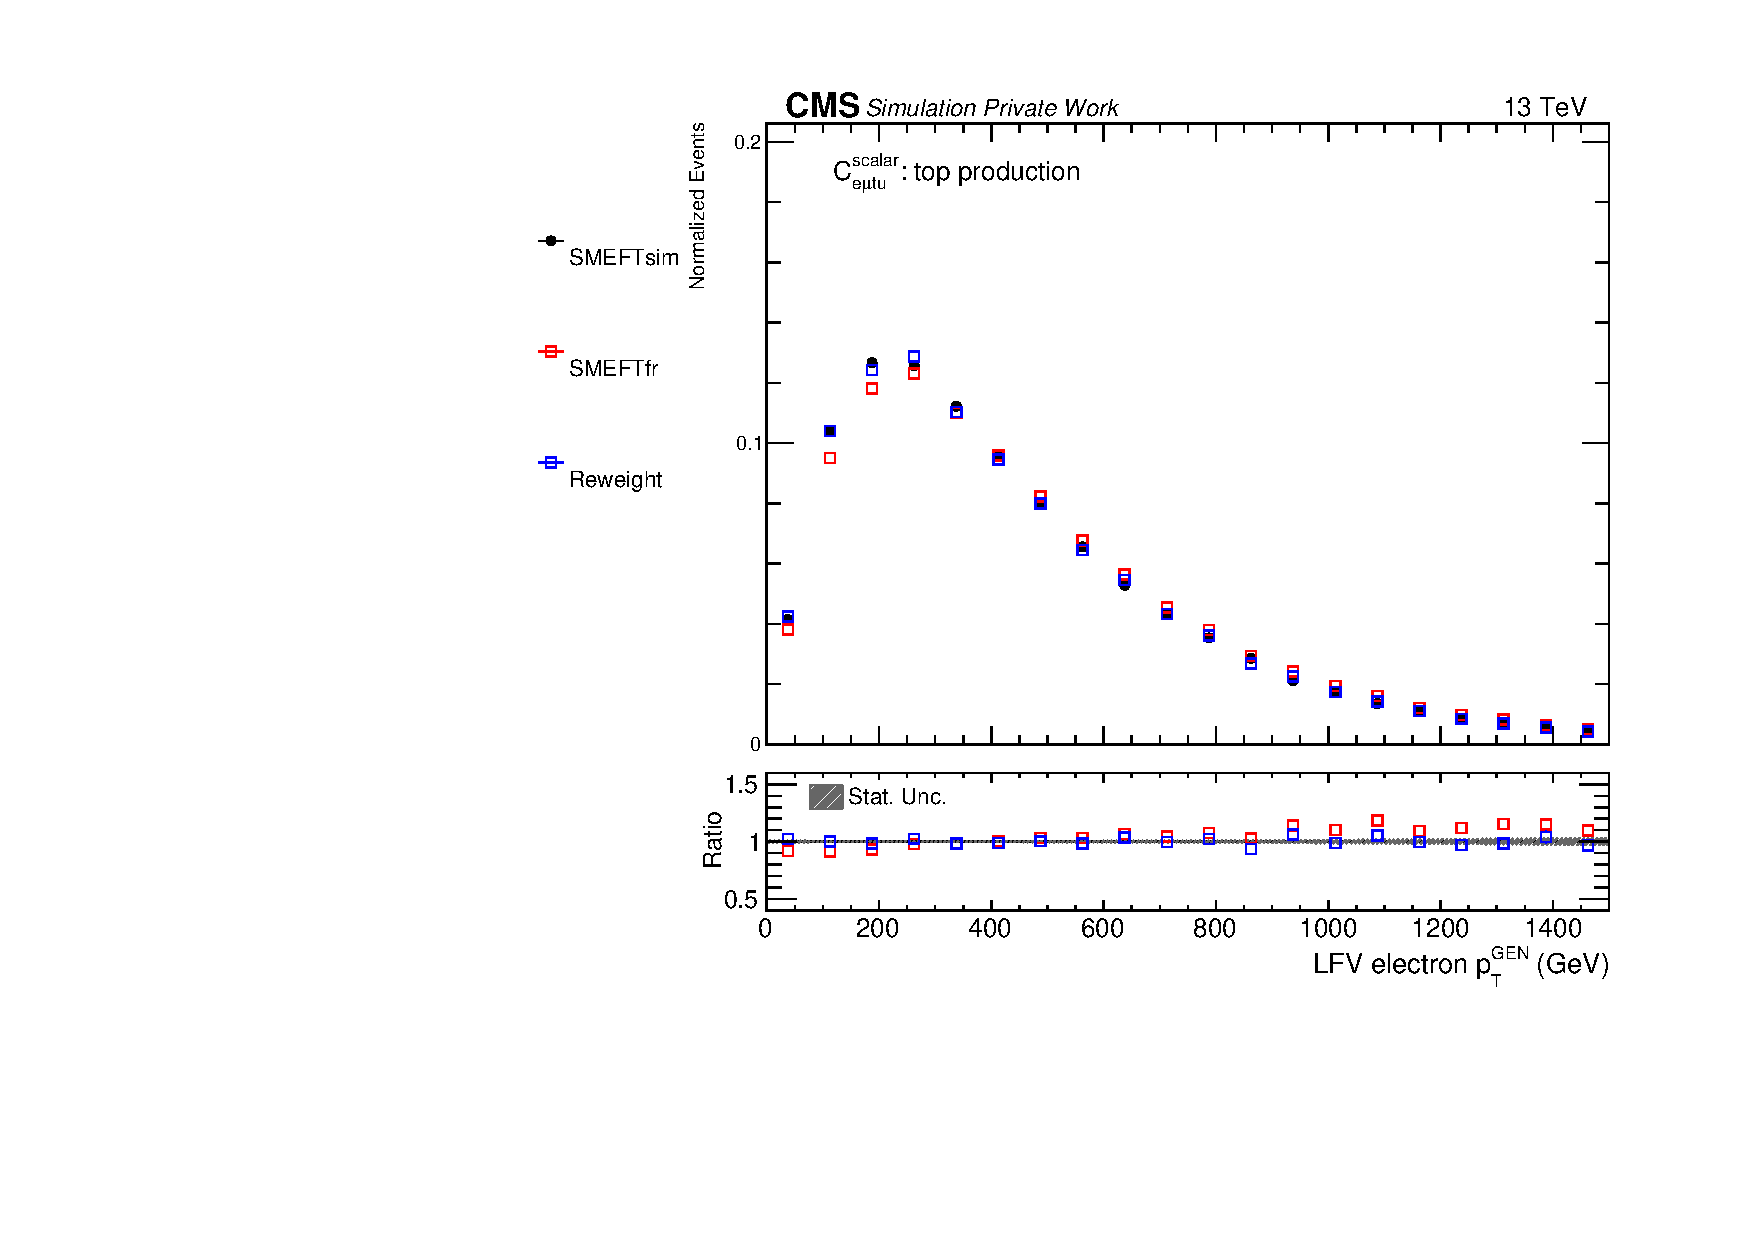
\includegraphics[width=0.48\textwidth]{figures/Part3/Samples/LFVePt}&
 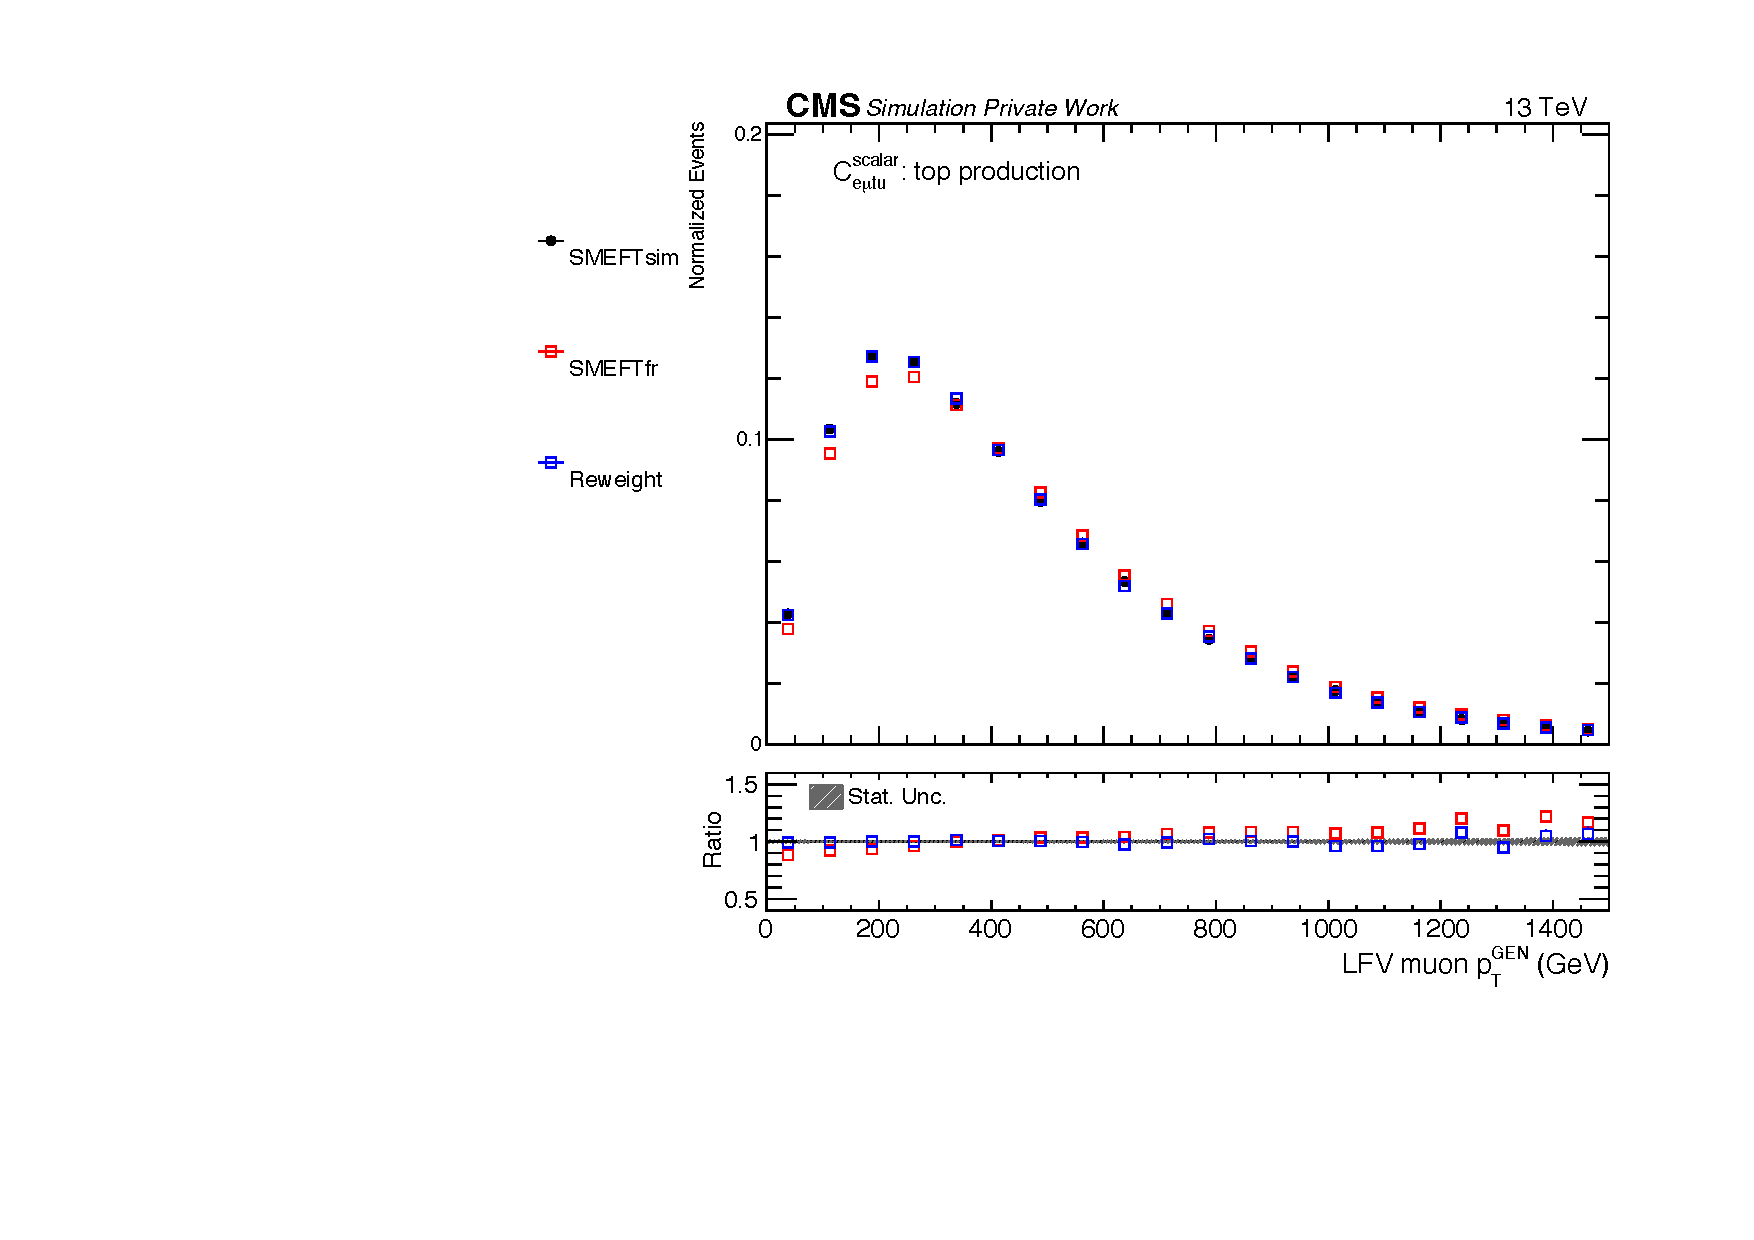
\includegraphics[width=0.48\textwidth]{figures/Part3/Samples/LFVmuPt}\\
 \end{tabular}
 \caption{Comparison of kinematic distributions at \ac{ME}-level produced by different models: LFV electron $\pt$ (left), LFV muon $\pt$ (right). The ``SmeftFR'' samples (shown in red curve) and ``SMEFTsim'' samples (shown in black curve) are statistically independent of each other. The ``Reweight'' (shown in blue curve) is produced by applying weights calculated by Equation~(\ref{eq:2}) to ``SmeftFR'' samples.}
 \label{fig:reweight}
 \end{center}
\end{figure}

In general, the calculations done by the \ac{ME} event generators are model-agnostic assuming the same \ac{EFT} configurations. In other words, models like SmeftFR or SMEFTsim~\cite{Brivio:2017btx} are expected to give the same or very similar results in terms of cross sections and four-momenta of final-state particles. Nevertheless, visible differences in kinematics have been observed and are shown in Figure~\ref{fig:reweight}. Furthermore, the cross sections predicted by SmeftFR v2 also yield more than 20\% difference relative to SMEFTsim due to a bug that was later fixed in SmeftFR v3. In light of these differences, the \ac{CMS} and \ac{ATLAS} Collaborations agreed to adopt the SMEFTsim model as the common standard. This decision was made after Ref.~\cite{CMS:2022ztx} has already been published, and Ref.~\cite{CMS:2022ztx} uses cross sections calculated by SmeftFR v2. To quantify the impact of the choice of models on kinematics, the following ratio is calculated for each event $i$,

\begin{equation}
\label{eq:2}
R_{\textsf{reweight}}^{i}=\frac{\omega_{\textsf{SMEFTsim}}^i}{\omega_{\textsf{SmeftFR}}^i},
\end{equation}

where $\omega^{i}_{X}$ is the per-event \ac{ME} weight calculated by \MG~using model $X$. Since SMEFTsim was not used by \ac{CMS} at the time when the signal samples were generated, $R_{\textsf{reweight}}$ are used to ``reweight'' the original samples generated using SmeftFR.

Due to the significant differences in kinematic distributions between top decay and production signals, \ac{MC} samples are generated separately for these processes. The cross sections for top production signals are taken directly from \MG~with SMEFTsim UFO as input. The event generation for top decay signals at the \ac{ME}-level takes two steps: (i) production of the SM $\ttbar$, and (ii) \ac{CLFV} decay of one of the top quarks. Therefore, the $\ttbar$ cross-section at \ac{NNLO} precision~\cite{Czakon:2011xx} is used to normalize the top decay signals,

\begin{equation}
\label{eq:3}
\sigma_{\textsf{CLFV}}^{\textsf{Top Decay}}=2\times\sigma_{\ttbar}^{\textsf{NNLO}}\times\mathcal{B}(\tto{q}),
\end{equation}

where q=\{u,c\}, and $\mathcal{B}(\tto{q})$ \cite{Kile:2008rp} can be expressed as,

\begin{equation}
\label{eq:4}
\mathcal{B}(\tto{q}) = 
\left\{ 
 \begin{array}{l}
 \displaystyle
 \frac{|\WC{\textsf{vector}}{\emut{q}}|^2}{\Lam^4}\frac{\textsf{m}_\textsf{t}^5}{384\pi^3\Gam_{\textsf{t}}^{\textsf{SM}}},\\
 \displaystyle
 \frac{|\WC{\textsf{scalar}}{\emut{q}}|^2}{\Lam^4}\frac{\textsf{m}_\textsf{t}^5}{3072\pi^3\Gam_{\textsf{t}}^{\textsf{SM}}}, \\
 \displaystyle
 \frac{|\WC{\textsf{tensor}}{\emut{q}}|^2}{\Lam^4}\frac{\textsf{m}_\textsf{t}^5}{64\pi^3\Gam_{\textsf{t}}^{\textsf{SM}}}, 
\end{array}
\right.
\end{equation}

where $\textsf{m}_{\textsf{t}}$ and $\Gam_{\textsf{t}}^{\textsf{SM}}$ are taken to be 172.5 GeV and 1.33 GeV in this analysis, respectively. The choice of u or c quark in final states does not affect the cross sections of the top decay signals. The cross sections for all signal \ac{MC} samples are summarized in Table~\ref{tab:signal}. These cross-sections are used as a baseline to define the signal strength $\mu$, which is used to quantify the relative strength of the signals when their normalization change,

\begin{equation}
\mu(\textsf{C}/\Lam^2)=\frac{\sigma_{\textsf{CLFV}}(\textsf{C}/\Lam^2)}{\sigma_{\textsf{CLFV}}(\textsf{1}\TeV^{-2})}\propto(\textsf{C}/\Lam^2)^2.
\label{eq:signal_strength}
\end{equation}

\begin{table}[th]
\sffamily
\centering
\caption{Theoretical cross sections for top production and decay for each \ac{CLFV} coupling, calculated at $\WC{}{}/\Lam^2$ = 1 \TeV$^{-2}$, $\mt = 172.5$ GeV, and $\mathrm{\Gamma}_{\textsf{t}}^{\textsf{SM}} = 1.33$ GeV by \MG~with SMEFTsim. The first uncertainty represents the effect of \ac{QCD} renormalization and factorization scales. The second uncertainty is the \ac{PDF} uncertainty.}
\begin{tabular}{clll}
\toprule 
Lorentz Structure & Samples    & XS (fb) \\ \midrule
\multirow{3}{*}{vector} & top production via u quark & $460^{+81}_{-64}\pm6$ \\ 
  & top production via c quark & $33^{+5}_{-4}\pm6$ \\
  & top decay via u/c quark  & $32.0^{+0.8}_{-1.1}\pm1.3$ \\ \midrule
\multirow{3}{*}{scalar} &top production via u quark & $97^{+18}_{-14}\pm1$ \\ 
  & top production via c quark  & $6.3^{+0.9}_{-0.8}\pm1.4$ \\
  & top decay via u/c quark & $4.0^{+0.1}_{-0.1}\pm0.2$ \\ \midrule 
\multirow{3}{*}{tensor} & top production via u quark & $2140^{+370}_{-290}\pm30$ \\
  & top production via c quark & $164^{+22}_{-18}\pm27$ \\
  & top decay via u/c quark  & $187^{+5}_{-6}\pm8$ \\ \bottomrule
\end{tabular}
\vspace{-0.5em}
\label{tab:signal}
\end{table}

Steps other than the \ac{ME} calculation concerning signal \ac{MC} generation follow the \ac{CMS} standard, which is described in the following section.
%%%%%%%%%%%%%%%%%%%%%%%%%%%%%%%%%%%%%%%%%%%%%%%%%%%%%%%%%%%%%
%%%%%%%%%%%%%%%%%%%%%%%%%%%%%%%%%%%%%%%%%%%%%%%%%%%%%%%%%%%%%
\section{Background Samples}
\label{sec:Backgrounds}

The background processes are divided into two categories: (i) processes with three or more \emph{prompt} leptons in the final states are classified as ``\emph{prompt} background'', and (ii) other processes are classified as ``\emph{nonprompt} background''. The \emph{nonprompt} backgrounds in this analysis are modeled with a data-driven technique, which is discussed in \autoref{chap:Nonprompt}. The \ac{MC} samples listed in the ``\emph{nonprompt}'' category in Table \ref{tab:MCsample} are therefore only used for validations. 

Besides tZq, tHq, tHW, and tWZ processes, the \ac{NLO} \ac{PDF} set from NNPDF3.0~\cite{NNPDF:2014otw} is used in 2016 to generate background \ac{MC} samples. The \ac{NNLO} \ac{PDF} set from NNPDF3.1~\cite{NNPDF:2017mvq} is used for tZq while the \ac{LO} \ac{PDF} set from NNPDF3.0 is used for tHq, tHW, and tWZ in 2016. In 2017 and 2018, the \ac{NNLO} \ac{PDF} set from NNPDF3.1 was used to generate all the samples. 

The default choice of \ac{ME} event generator is \MG~v2.4.2 (v2.2.2 for 2016), which is used to generate all but ZZ, $\ttbar$H, and $\ttbar$ samples. These three samples are generated with \Pow~v2~\cite{Frixione:2007vw} instead. Samples with small contributions (tHq, tWZ, tHW, and low mass \ac{DY} ) are generated at \ac{LO} while other samples are generated at \ac{NLO}. Whenever possible and relevant, theoretical cross sections from high-order \ac{QCD} calculations are used. The references of these calculations are included in \ref{tab:MCsample}.

The \PY~v8.2~\cite{Sjostrand:2014zea} is used to model parton shower and hadronization. The CUETP8M1~\cite{CMS:2015wcf} was used in 2016 for underlying event tuning while the CP5~\cite{CMS:2019csb} was used in 2017 and 2018. The configurations of the \ac{MC} samples are summarized in Table \ref{tab:MCsample}. 

\begin{table}
\sffamily
\caption{Summary of the configurations of the \ac{MC} samples. DYM50 (DYM10to50) denotes a \ac{DY} sample with a dilepton invariant mass greater than 50 GeV (between 10 and 50 GeV). V includes W and Z bosons. The cross-sections for samples without a citation are taken directly from their event generators.}
\centering
 \resizebox{\linewidth}{!}{%
 \begin{tabular}{cccccc}
\toprule
Category & Process & Event Generator & Perturbative QCD& Tune & XS precision \\ \midrule
\multirow{7}{*}{\vtop{\hbox{\strut~~\emph{prompt}}\hbox{\strut background}}}  
 & WZ & \textsc{MadGraph} & NLO & CUETP8M1(CP5) & NLO~\cite{Campbell:2011bn} \\ 
 & ZZ & \textsc{powheg} & NLO & CUETP8M1(CP5) & NLO~\cite{Campbell:2011bn} \\
 &VVV & \textsc{MadGraph} & NLO & CUETP8M1(CP5) & NLO \\ 
 & $\ttbar$W, $\ttbar$Z & \textsc{MadGraph} & NLO & CUETP8M1(CP5) & NLO~\cite{Frederix:2021agh,Kulesza:2020nfh} \\
 & $\ttbar$H & \textsc{powheg} & NLO & CUETP8M1(CP5) & NLO~\cite{Kulesza:2020nfh} \\ 
 & tZq & \textsc{MadGraph} & NLO & CP5 & NLO \\
 & tHq, tHW, tWZ & \textsc{MadGraph} & LO & CUETP8M1(CP5) & LO \\
 \midrule
 \multirow{3}{*}{\vtop{\hbox{\strut \emph{nonprompt}}\hbox{\strut background}}}
 & $\ttbar$ & \textsc{powheg} & NLO & CUETP8M1(CP5) & NNLO~\cite{Czakon:2011xx} \\ 
 & DYM50 & \textsc{MadGraph} & NLO & CUETP8M1(CP5) & NNLO~\cite{Li:2012wna} \\
 & DYM10to50 & \textsc{MadGraph} & LO & CUETP8M1(CP5) & NLO~\cite{Li:2012wna} \\
 \bottomrule
 \end{tabular}}
 \label{tab:MCsample}
 \end{table} 
 
 All simulated events include a detailed simulation of the CMS detector response based on \textsc{Geant4}~\cite{GEANT4:2002zbu}, and are processed using the same \ac{CMS} event reconstruction software as used for the data.
 %%%%%%%%%%%%%%%%%%%%%%%%%%%%%%%%%%%%%%%%%%%%%%%%%%%%%%%%%%%%%
%%%%%%%%%%%%%%%%%%%%%%%%%%%%%%%%%%%%%%%%%%%%%%%%%%%%%%%%%%%%%
\section{Triggers}
\label{sec:Triggers}

The target final states of this analysis contain three prompt leptons, which make lepton triggers the most optical choice to select events. To achieve maximum acceptance, a combination of single-lepton, di-lepton, and tri-lepton triggers are used. These triggers are summarized in \autoref{chap:Triggers}. Events in simulated samples are required to fire at least one of the triggers listed in Table~\ref{tab:triggers16}-\ref{tab:triggers18}. Since multiple \acp{PD} are used to record data events and the orthogonality of these \acp{PD} is not guaranteed by the online selection criteria, the following trigger logic is implemented to remove the overlap between different \acp{PD}:

\begin{itemize}
\item Events in SingleMuon datasets are required to fire at least one of the triggers listed under ``SingleMuon''. 
\item Events in DoubleMuon datasets are required to fire at least one of the triggers listed under ``DoubleMu''. Events are removed if they also fire at least one of the triggers listed under ``SingleMuon''.
\item Events in ``MuonEG'' datasets are required to fire at least one of the triggers listed under ``MuonEG''. Events are removed if they also fire at least one of the triggers listed under ``SingleMuon'' or ``DoubleMu''.
\item Events in Single Electron datasets are required to fire at least one of the triggers listed under ``SingleElectron''. Events are removed if they also fire at least one of the triggers listed under ``SingleMuon'', ``DoubleMu'', or ``MuonEG''.
\item Events in DoubleEG datasets are required to fire at least one of the triggers listed under ``DoubleEG''. Events are removed if they also fire at least one of the triggers listed under ``SingleMuon'', ``DoubleMu'', ``MuonEG'', or ``SingleElectron''.
\item Events in EGamma datasets are required to fire at least one of the triggers listed under ``EGamma''. Events are removed if they also fire at least one of the triggers listed under ``SingleMuon'', ``DoubleMu'', or ``MuonEG''.
\end{itemize}
\chapter{Object Selection}
\label{chap:Objects}

Objects described in \autoref{chap:Reco}, referred to as ``candidates'', are further selected with more stringent requirements to suppress the contributions from background processes while maintaining a high signal acceptance. In particular, prompt electron and muon candidates are identified through a custom-trained \ac{BDT} classifier, which is discussed in \autoref{sec:Leptons}. Two jet identification algorithms are deployed to select jet candidates originating from hard collisions, which is discussed in \autoref{sec:Jets}. Furthermore, jet candidates that originate from b quarks are identified with a \ac{NN} based algorithm, which is discussed in \autoref{sec:Btag}. 
%%%%%%%%%%%%%%%%%%%%%%%%%%%%%%%%%%%%%%%%%%%%%%%%%%%%%%%%%%%%%
%%%%%%%%%%%%%%%%%%%%%%%%%%%%%%%%%%%%%%%%%%%%%%%%%%%%%%%%%%%%%
\section{Lepton Selection}
\label{sec:Leptons}

The target final states of this analysis feature exactly three leptons that originate either from decays of electroweak bosons or from the \ac{CLFV} interaction, which in this analysis is a contact interaction that involves four fermions. These leptons, referred to as \emph{prompt} leptons, typically appear to be isolated and not far away from the \ac{PV}. In contrast, \emph{nonprompt} leptons are leptons that originate from decays of hadrons, or photon conversions, or misidentified leptons. They often travel a noticeable distance away from the \ac{PV} and appear to be less isolated due to nearby activities. Due to the high multiplicity of leptons in our selection, backgrounds with at least one \emph{nonprompt} lepton outnumber any other \ac{SM} processes that produce three or more \emph{prompt} leptons. It is therefore crucial to exploit the differences between \emph{nonprompt} and \emph{prompt} leptons and bring the \emph{nonprompt} background under control. 
%%%%%%%%%%%%%%%%%%%%%%%%%%%%%%%%%%%%%%%%%%%%%%%%%%%%%%%%%%%%%
\subsection{TOP LeptonMVA}
\label{sec:TOPMVA}

The \TOP is an offline lepton identification algorithm that was originally developed for tZq analyses \cite{CMS:2018sgc,CMS:2021ugv}. It is based on Gradient \ac{BDT} implemented using the TMVA package~\cite{TMVA:2007ngy}. A total of 13 features are used as input to the \ac{BDT}. They can be categorized into four groups: (i) positions and momenta of the lepton candidates, (ii) isolation variables, (iii) variables associated with the closest jet, and (iv) a quality variable that is specific to electron or muon candidate. The version of \TOP used by this analysis is the same as \cite{CMS:2021ugv}, where a detailed description of all input features can be found.

\emph{Prompt} leptons from $\ttbar$W, $\ttbar$Z, and tZq samples are used as signals in the \ac{BDT} training while \emph{nonprompt} leptons from $\ttbar$ samples are used as backgrounds. The trained \ac{BDT} outputs a single score for each lepton candidate ranging from -1 to 1 with -1 (1) being the most background- (signal-) like. the tight working point with a threshold of ($>$) 0.9 is chosen as the selection criteria for both electron candidates and muon candidates, which corresponds to a signal(background) efficiency of 90\%(1\%). The strategy is to trade a small percentage (<10\%) of signal efficiency for several factors of background rejection. 
%%%%%%%%%%%%%%%%%%%%%%%%%%%%%%%%%%%%%%%%%%%%%%%%%%%%%%%%%%%%%
\subsection{Full Selection}
In addition to the \TOP requirement, a set of common selection criteria is applied to both electron and muon candidates. The minimum $\pt$ requirement is 38GeV, 20 GeV, and 20 GeV for the leading, sub-leading, and trailing lepton in $\pt$, respectively. This requirement is driven by the $\pt$ thresholds of the \ac{HLT} triggers to avoid inefficiency at turn-on. Electron and muon candidates are required to be in the pseudorapidity range $|\eta|<$2.4, which corresponds to the acceptance of \ac{CMS} tracker and muon system in 2016-2018. The transverse (longitudinal) impact parameters with respect to the \ac{PV}, denoted as $d_{\textsf{xy}}$ ($d_{\textsf{z}}$), is required to be in the range $|d_{\textsf{xy}}|~<$ 0.05 cm ($|d_{\textsf{z}}|~<$ 0.05 cm). The significance of the 3-dimensional impact parameter, denoted as SIP$_3$, is defined as the 3-dimensional impact parameter divided by its uncertainty. It is required that SIP$_3$ $<$ 8. The three cuts on impact parameters are added due to the difference in distributions of these parameters between \emph{prompt} and \emph{nonprompt} leptons. Also, they are part of the pre-selection requirement in the \ac{BDT} training.

Furthermore, all lepton candidates are required to be isolated. This is achieved by first defining a cone with a distance parameter of $\mathrm{\Delta}R$ around each lepton candidate, where $\mathrm{\Delta}R=\sqrt{\mathrm{\Delta}\eta^2+\mathrm{\Delta}\phi^2}$. Only particles within $\mathrm{\Delta}R<R_{\textsf{max}}$ can contribute to the isolation variable, where $R_{\textsf{max}}$ is referred to as the size of the cone. Secondly, a \ac{PF} based isolation variable is defined as,

\begin{equation}
I^{\textsf{rel}}_{\textsf{mini}} = \frac{1}{p_{\textsf{T}}^{\ell}} \{\sum_{\textsf{charged}}\pt+\max(0,\sum_{\textsf{neutral}}\pt-\rho \mathcal{A}[\frac{\mathrm{\Delta}R}{0.3}]^2)\},
\end{equation}

where $p_{\textsf{T}}^{\ell}$ is the $\pt$ of the lepton candidate, the first term inside the curly braces is the scalar sum of all charged particles associated with the \ac{PV} while the second term evaluates the contribution from neutral particles. This is done by first scalar-summing over $\pt$ of all neutral particles associated to the \ac{PV}. A correction term, known as effective area correction~\cite{Cacciari:2007fd}, is then subtracted. This term is used to mitigate the impact of \ac{PU} interactions. The size of the cone scales with $p_{\textsf{T}}^{\ell}$ as,  

\begin{equation}
R_{\textsf{max}} = \max (0.05, \min(0.2, \frac{10\GeV}{p_{\textsf{T}}^{\ell}})).
\end{equation}.

This type of isolation variable is known as ``mini'' isolation, which maximizes the signal efficiency at $p_{\textsf{T}}^{\ell}$ by reducing the cone size. It is required that lepton candidates to have $I^{\textsf{rel}}_{\textsf{mini}}<$ 0.12.

For electron specifically, candidates are required to have a GSF track with one or less missing inner hits. Electron candidates reconstructed in the transition region between ECAL barrel and endcap (i.e. 1.44 $<~|\eta_{\textsf{SC}}|~<$ 1.57) are removed from consideration. For muon specifically, candidates are required to be \ac{PF} muons and pass the medium working point discussed in \autoref{sec:Muon}.

Lepton candidates that pass all requirements stated above are referred to as ``\emph{tight}'' leptons. Leptons selected with a separate set of criteria, known as ``\emph{loose}'', is used in estimating the \emph{nonprompt} background, which is discussed in \autoref{chap:Nonprompt}. Unless explicitly stated, all lepton objects presented in this search are \emph{tight} leptons.

The energy scale and resolution is calibrated for all electron candidates, as discussed in \autoref{sec:Electron}. The energy scale and resolution is also calibrated for muon candidates with $\pt~<$ 200 GeV, as discussed in \autoref{sec:Muon}. Per-object scale factors are applied to \emph{tight} leptons in simulated events to correct for the differences in reconstruction, isolation, and identification between data and \ac{MC}. These scale factors are obtained using dilepton events in the Z resonance window.
%%%%%%%%%%%%%%%%%%%%%%%%%%%%%%%%%%%%%%%%%%%%%%%%%%%%%%%%%%%%%
%%%%%%%%%%%%%%%%%%%%%%%%%%%%%%%%%%%%%%%%%%%%%%%%%%%%%%%%%%%%%
\section{Jet Selection}
\label{sec:Jets}

Jet candidates are reconstructed from \ac{PF} candidates using the anti-$k_{\textsf{T}}$ algorithm described in \autoref{sec:Jets} with a cone size of 0.4. Charged hadrons that are not associated to the \ac{PV} are removed. Jet candidates are required to have a minimum $\pt$ of 30 GeV and in the pseudorapidity range $|\eta|<$2.4, where b-tagging is still effective. It is further required that all jet candidates be isolated from \emph{tight} leptons. A cone of the size 0.4 around each jet candidate is defined and candidates will be removed if any \emph{tight} leptons are found within such a cone. This procedure is implemented to remove the overlap between leptons and jets. 

The two primary sources of background are (i) detector noise, and (ii) jets from \ac{PU} interactions. To suppress detector noise, a set of cut-based selections is applied to jet candidates. This algorithm utilizes information from \ac{PF} candidates, including: (i) fraction of charged (neutral) hadrons energy, (ii) fraction of charged (neutral) EM energy, (iii) fraction of muon energy, and (iv) object multiplicity. The ``tightLepVeto'' working point is chosen to select jet candidates, which corresponds to 98-99\% signal efficiency.

The second algorithm is designed to reject jet candidates that originate from \ac{PU} interactions. This algorithm is based on a \ac{BDT} that utilizes: (i) the trajectories of tracks associated to the jets, (ii) the topology of the jet shape, and (iii) object multiplicity. The \emph{loose} working point is chosen to select jet candidates with $\pt~<$ 50 GeV, which corresponds to 99\% signal efficiency. Applying this algorithm to jet candidates with $\pt~>$ 50 GeV is both ineffective and unnecessary as \ac{PU} jets mostly reside in the low $\pt$ spectrum. The overall effect of this algorithm on this analysis is small as \ac{PU} jets constitute only a small fraction of all jet candidates in the phase space of this analysis. 

As discussed in \autoref{sec:Jet}, the energy scale for all jet candidates (data and \ac{MC}) are calibrated. One extra correction is applied to simulated jets to recreate the jet energy resolution as measured in the data. 
%%%%%%%%%%%%%%%%%%%%%%%%%%%%%%%%%%%%%%%%%%%%%%%%%%%%%%%%%%%
%%%%%%%%%%%%%%%%%%%%%%%%%%%%%%%%%%%%%%%%%%%%%%%%%%%%%%%%%%%

\section{Identification of b jets}
\label{sec:Btag}

The \DeepJ algorithm~\cite{Bols:2020bkb} is used to identify jets that originate from b quark. The core strategy of this algorithm is to minimize information. This is achieved by removing entirely the selection of jet constituents, which limits the number of jet constituents considered. Additionally, an effort is made to use as many low-level features as possible, which further further deepens the feature space. Approximately a total of 650 input features are used, which can be categorized into four groups: (i) global variables, (ii) charged PF candidate features, (iii) neutral PF candidate features, (iv) and \ac{SV} features associated with the jet. When compared to the existing \DeepC algorithm~\cite{CMS:2017wtu}, \DeepJ algorithm delivers up to 20\% improvement in signal efficiency while maintaining the same background efficiency.

The \DeepJ algorithm outputs a score ranging between 0 and 1, with 0 (1) being the most background- (signal-) like. The medium working point is chosen to tag b jet candidate, which corresponds to 70\%-80\% signal efficiency. The shape of the \DeepJ output distribution is corrected for the differences between data and \ac{MC} in signal and background efficiencies. The per-event correction weight $ \omega$ is defined as,
 
 \begin{equation}
 \omega = \prod_{i}^{N_{\textsf{jets}}} \textsf{SF}(p_{T_{i}},\eta_i, F_i, D_i),
 \end{equation}
 
where \textsf{SF} is the ratio of efficiency in data to efficiency to \ac{MC} parameterized as a function of $\pt$, $\eta$, (MC truth) flavor F, as well as \DeepJ output $D$ of each jet in the event. $\omega$ is applied to all \ac{MC} events.

Additional corrections are applied to remove the normalization effect of $\omega$ before jet selection. These scale factors are measured using \ac{MC} in e$\upmu\ell$ channel described in \autoref{chap:Selection}. The effect of these scale factors is shown in Figure~\ref{fig:BtagSF}.
 
 \begin{figure}[tbh!]
 \begin{center}
 \begin{tabular}{c}
 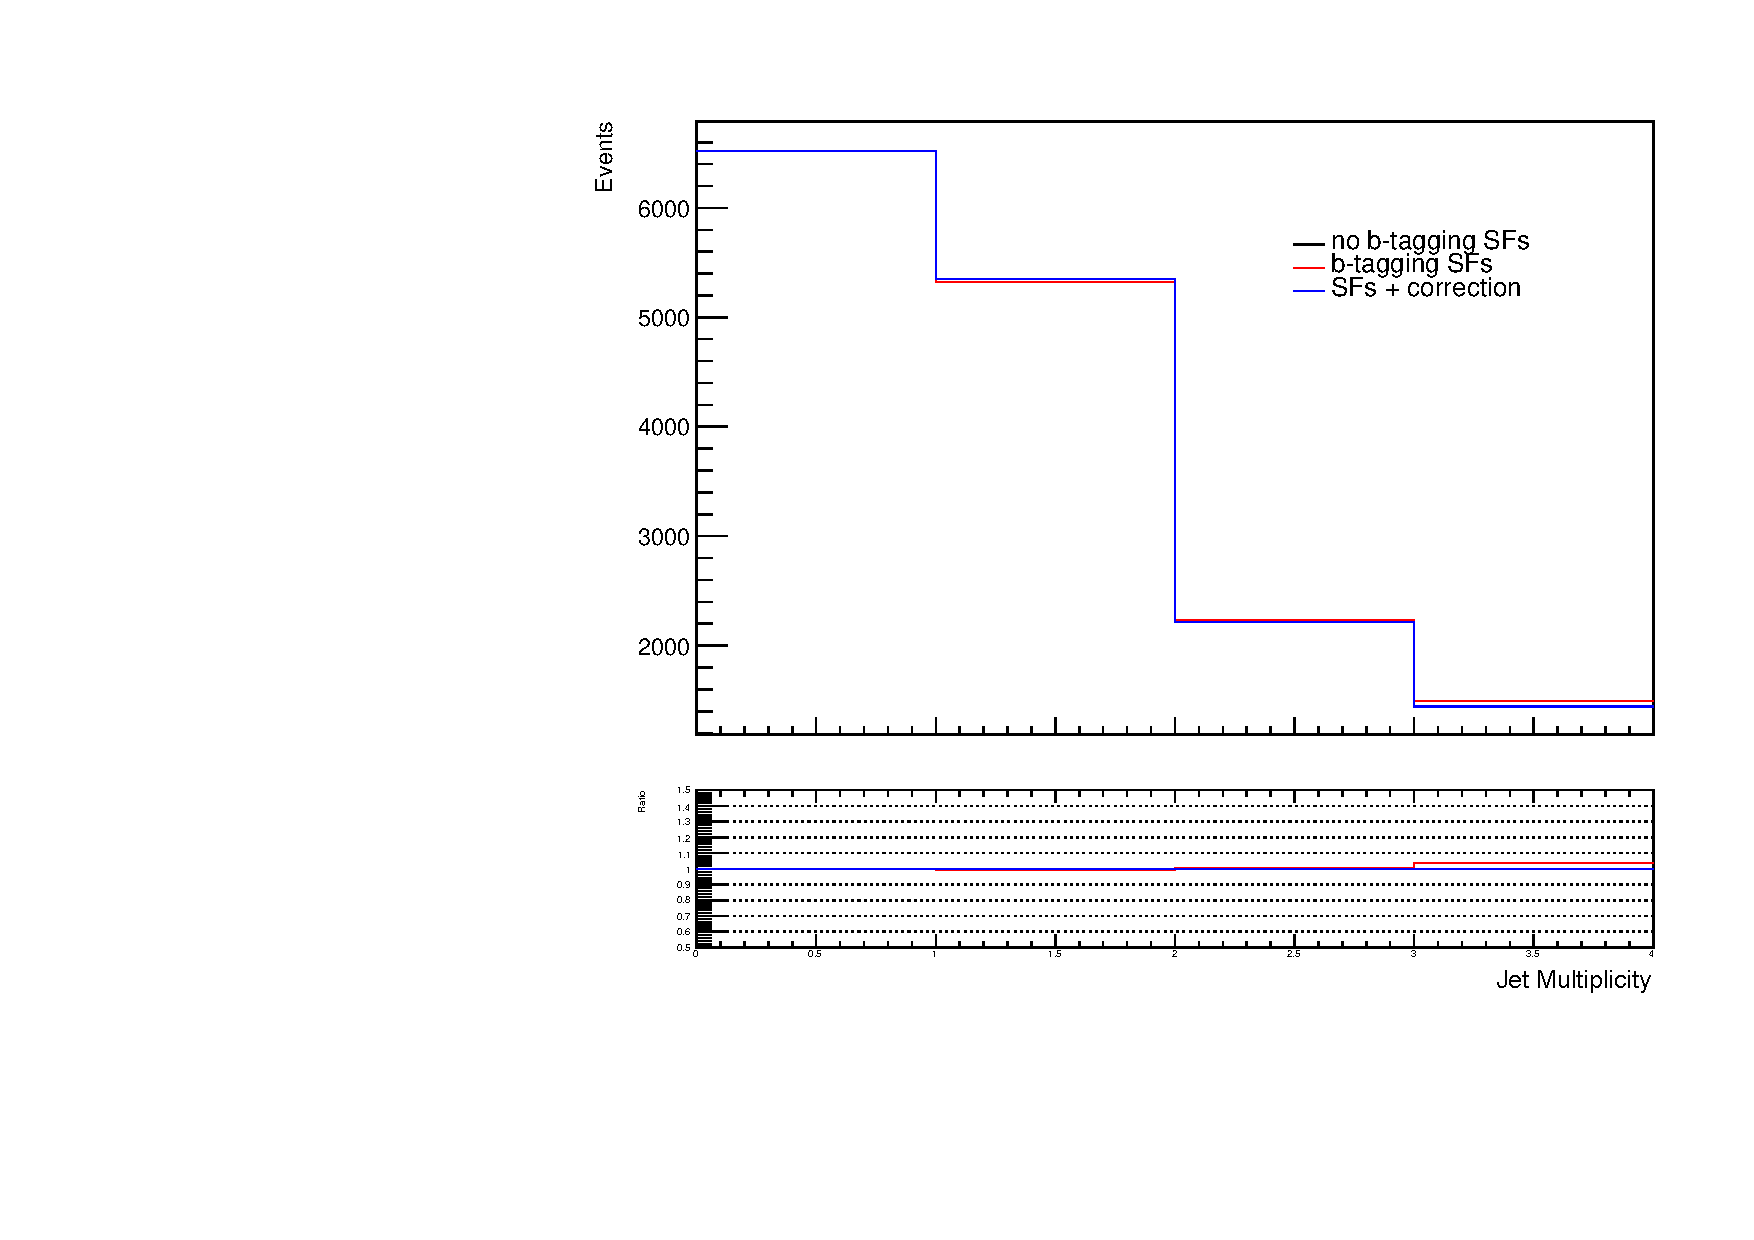
\includegraphics[width=0.75\textwidth]{figures/Part3/Objects/njet_Btag}\\
 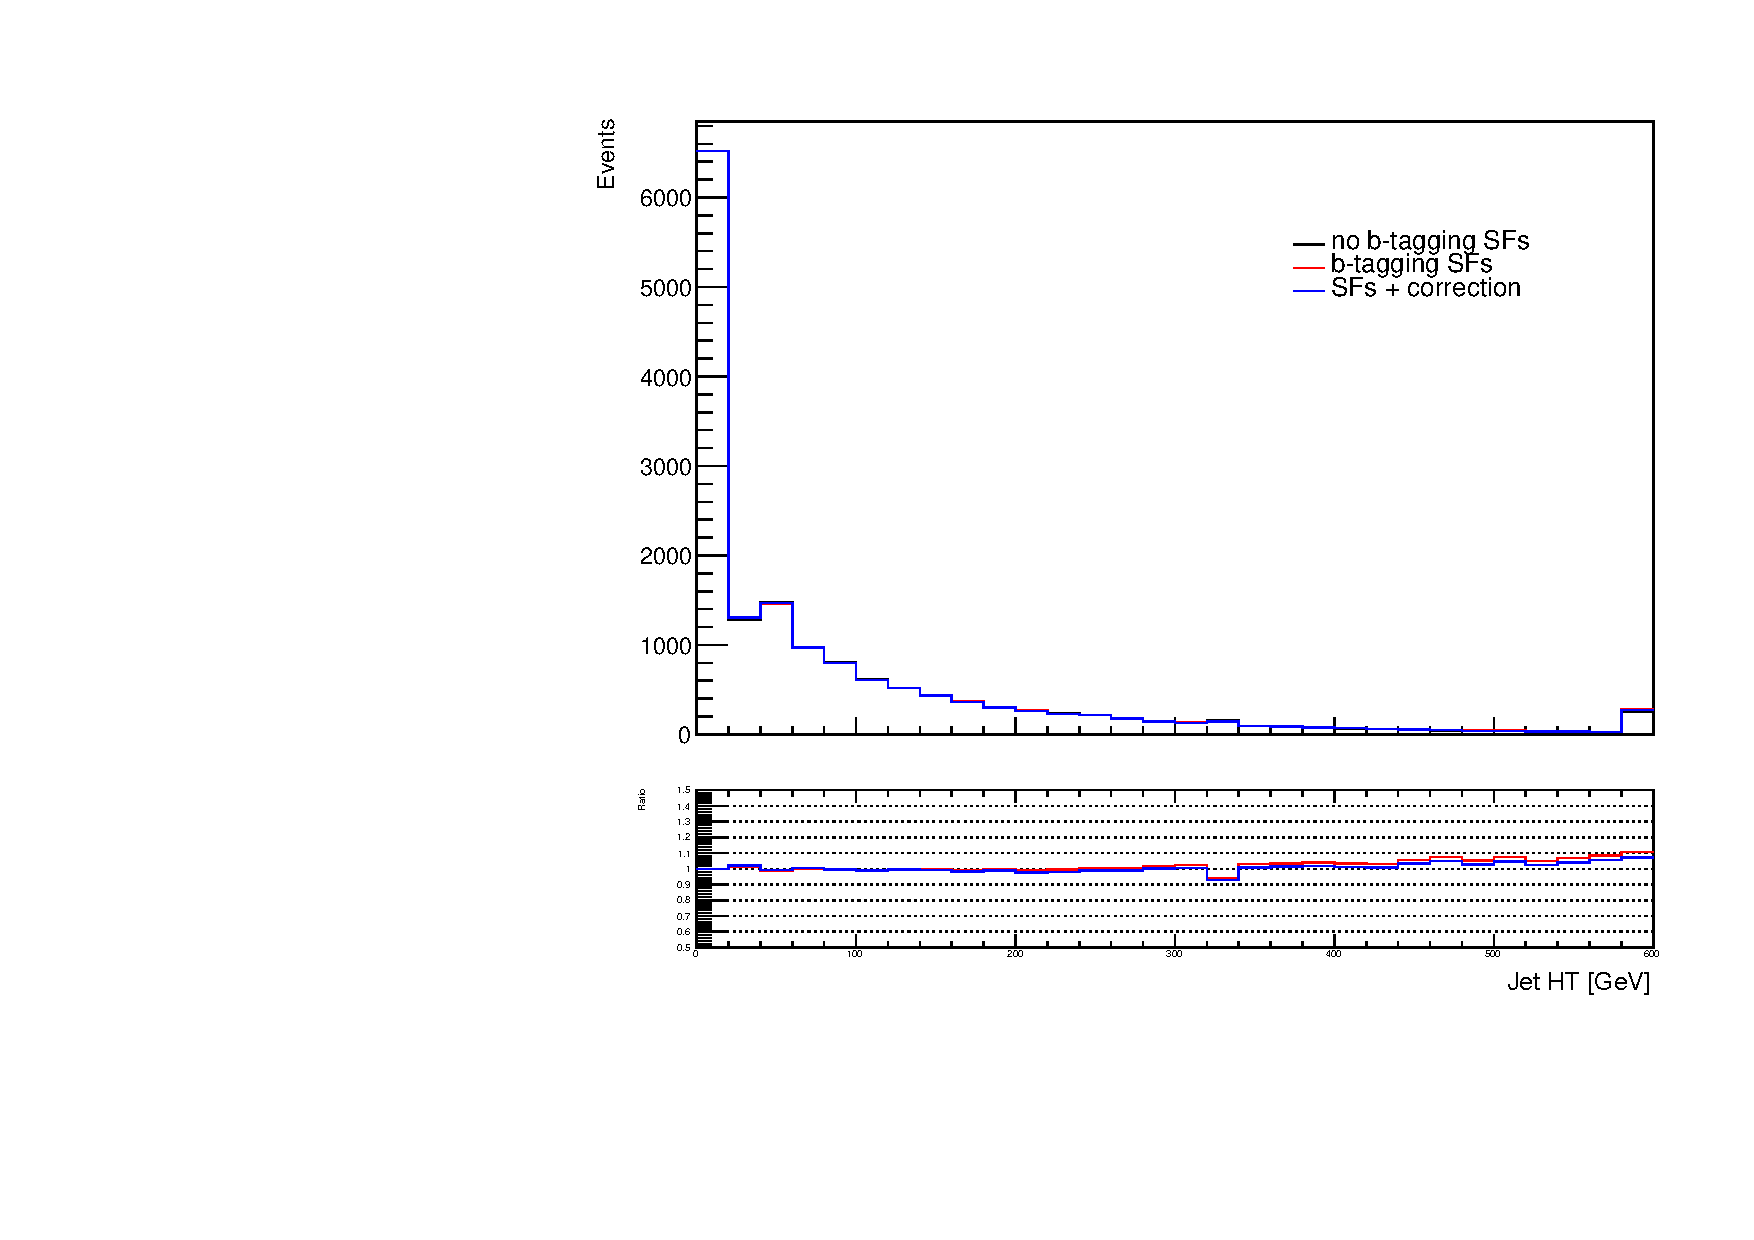
\includegraphics[width=0.75\textwidth]{figures/Part3/Objects/Ht_Btag} \\
 \end{tabular}
 \caption{Simulated events in $\emul$ channel without additional requirements on jets. The top histogram shows distribution of jet multiplicity while the bottom histogram shows the distribution of $H_\textsf{T}$, which denotes the scalar sum of the $\pt$ of all jets. Distributions without any jet-related scale factors are shown in black lines. Distributions with only b-tagging scale factors are shown in red lines. Distributions with b-tagging scale factors and corrections to remove normalization effects are shown in blue lines.}
 \label{fig:BtagSF}
 \end{center}
\end{figure}
\chapter{Event Selection}
\label{chap:Selection}

Events are required to contain exactly three \emph{tight} leptons described in \autoref{sec:Leptons}. Furthermore, events are selected with \ac{HLT} triggers discussed in \autoref{sec:Triggers}. Events with different lepton flavor composites are further categorized into three exclusive channels: eee, $\mmm$, $\emul$. In all three channels, the sum of the electric charges of the selected leptons is required to be 1 or -1. The leading leptons in all selected events are required to be matched with trigger objects within $\mathrm{\Delta} R~<$ 0.2. Within each channel, different regions are defined to further understand signal and background.

$\emul$ is the channel where close to 100\% of the simulated signal events reside. This channel is divided into signal-enriched \acp{SR} and signal-depleted \acp{VR}, which are discussed in \autoref{sec:SR} and \autoref{sec:VR}, respectively. Due to the lack of different flavors, the eee and $\mmm$ channels are signal-depleted by definition. Therefore, events found in these two channels are only used to study background processes, which are discussed in \autoref{sec:VR}. The kinematic reconstruction of heavy particles, such as the top quark, is described in \autoref{sec:Kin}.
%%%%%%%%%%%%%%%%%%%%%%%%%%%%%%%%%%%%%%%%%%%%%%%%%%%%%%%%%%%%%
%%%%%%%%%%%%%%%%%%%%%%%%%%%%%%%%%%%%%%%%%%%%%%%%%%%%%%%%%%%%%
\section{Signal Region}
\label{sec:SR}

The core feature of the signal events is the presence of the ``LFV e$\upmu$'' pair, which consists of a pair of \ac{OSDF} leptons. It is guaranteed that there is at least one \ac{OSDF} pair in all events residing in the $\emul$ channel due to the requirement on electric charges. The \ac{OSDF} pair is immediately labeled as the LFV e$\upmu$ pair if it is only possible to reconstruct one \ac{OSDF} pair. In events where a pair of \ac{SSSF} leptons are present, a kinematic reconstruction is used to determine which one of two leptons form the LFV e$\upmu$ pair with the third lepton, which is detailed in \autoref{sec:Kin}. Leptons that form the LFV e$\upmu$ pair are referred to as the LFV electron or muon as it is assumed that they originate from the \ac{CLFV} interaction. Based on the event topology of the signal process, further selection criteria are applied to define the \ac{SR}. These selection criteria help achieve an optimal signal-to-background ratio by removing the majority of the background events present in the $\emul$ channel. 

At the tree level, signal events are expected to contain one or two jets, which motivates a requirement of at least one jet in \ac{SR}. Furthermore, it is required that there is no more than one b-tagged jet to suppress the contribution from $\ttbar$ events. Another prominent background is \ac{DY} production that features an \ac{OSSF} pair. To suppress \ac{DY} processes in \ac{SR}, events that contain an \ac{OSSF} lepton pair with an invariant mass between 50 GeV and 106 GeV are removed. The lower bound of this veto is lower than the typical value (e.g. 75 GeV) because the mass range between 50 GeV and 75 GeV has very few signal events and is dominated by \emph{nonprompt} background from photon conversion. Additionally, a modest threshold of 20 GeV is applied to \MET~due to the presence of neutrinos in the signal events.

Distributions of the LFV e$\upmu$ mass and the mass of the \ac{OSSF} lepton pair are shown in Figure~\ref{fig:SR}. All backgrounds in Figure~\ref{fig:SR} are estimated using \ac{MC} simulation even though the strategy is to use a data-driven method to estimate the \emph{nonprompt} background. This serves as a preliminary check to understand the components of different backgrounds in \ac{SR}. Distributions of more variables in \ac{SR} are included in \autoref{chap:SRMC}.

\begin{figure}[tbh!]
 \begin{center}
 \begin{tabular}{cc}
 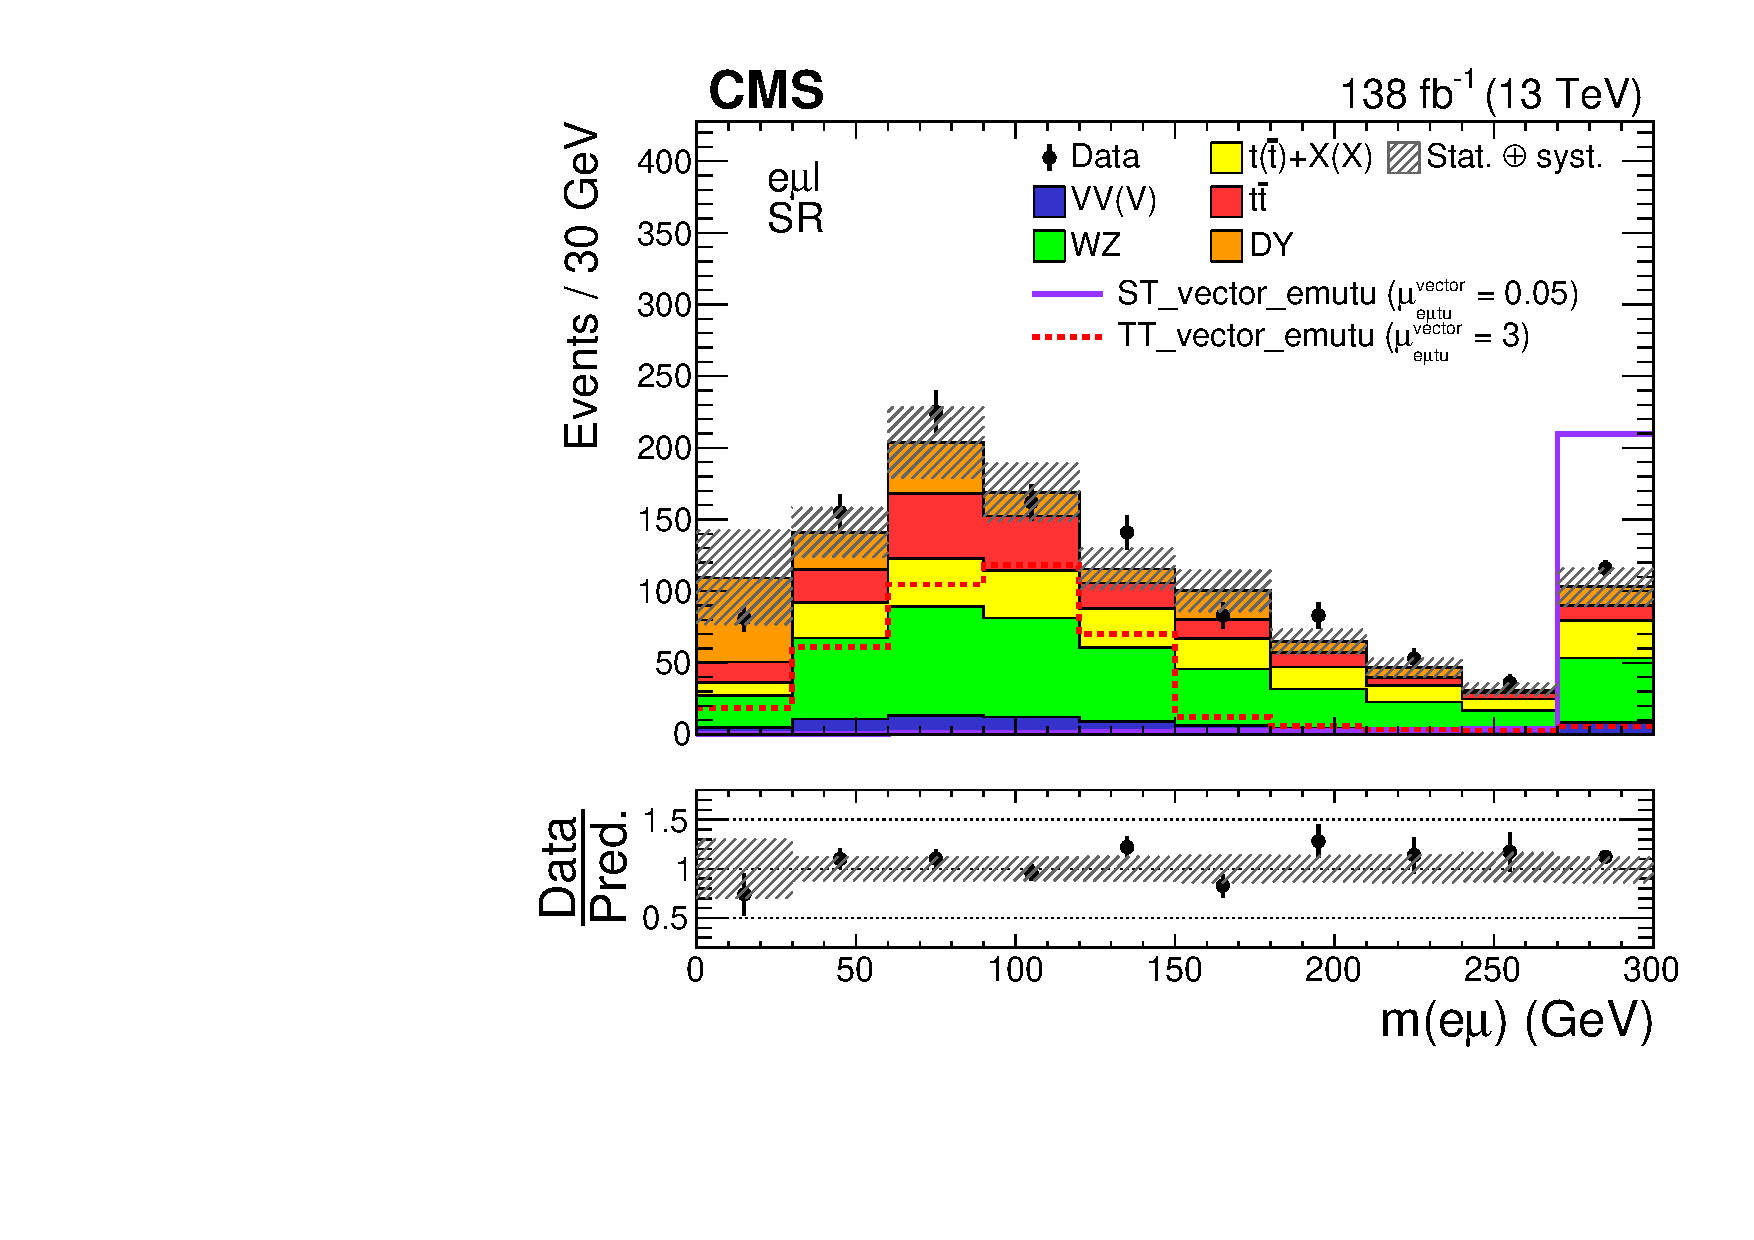
\includegraphics[width=0.48\textwidth]{figures/Part3/Selection/Memu}&
 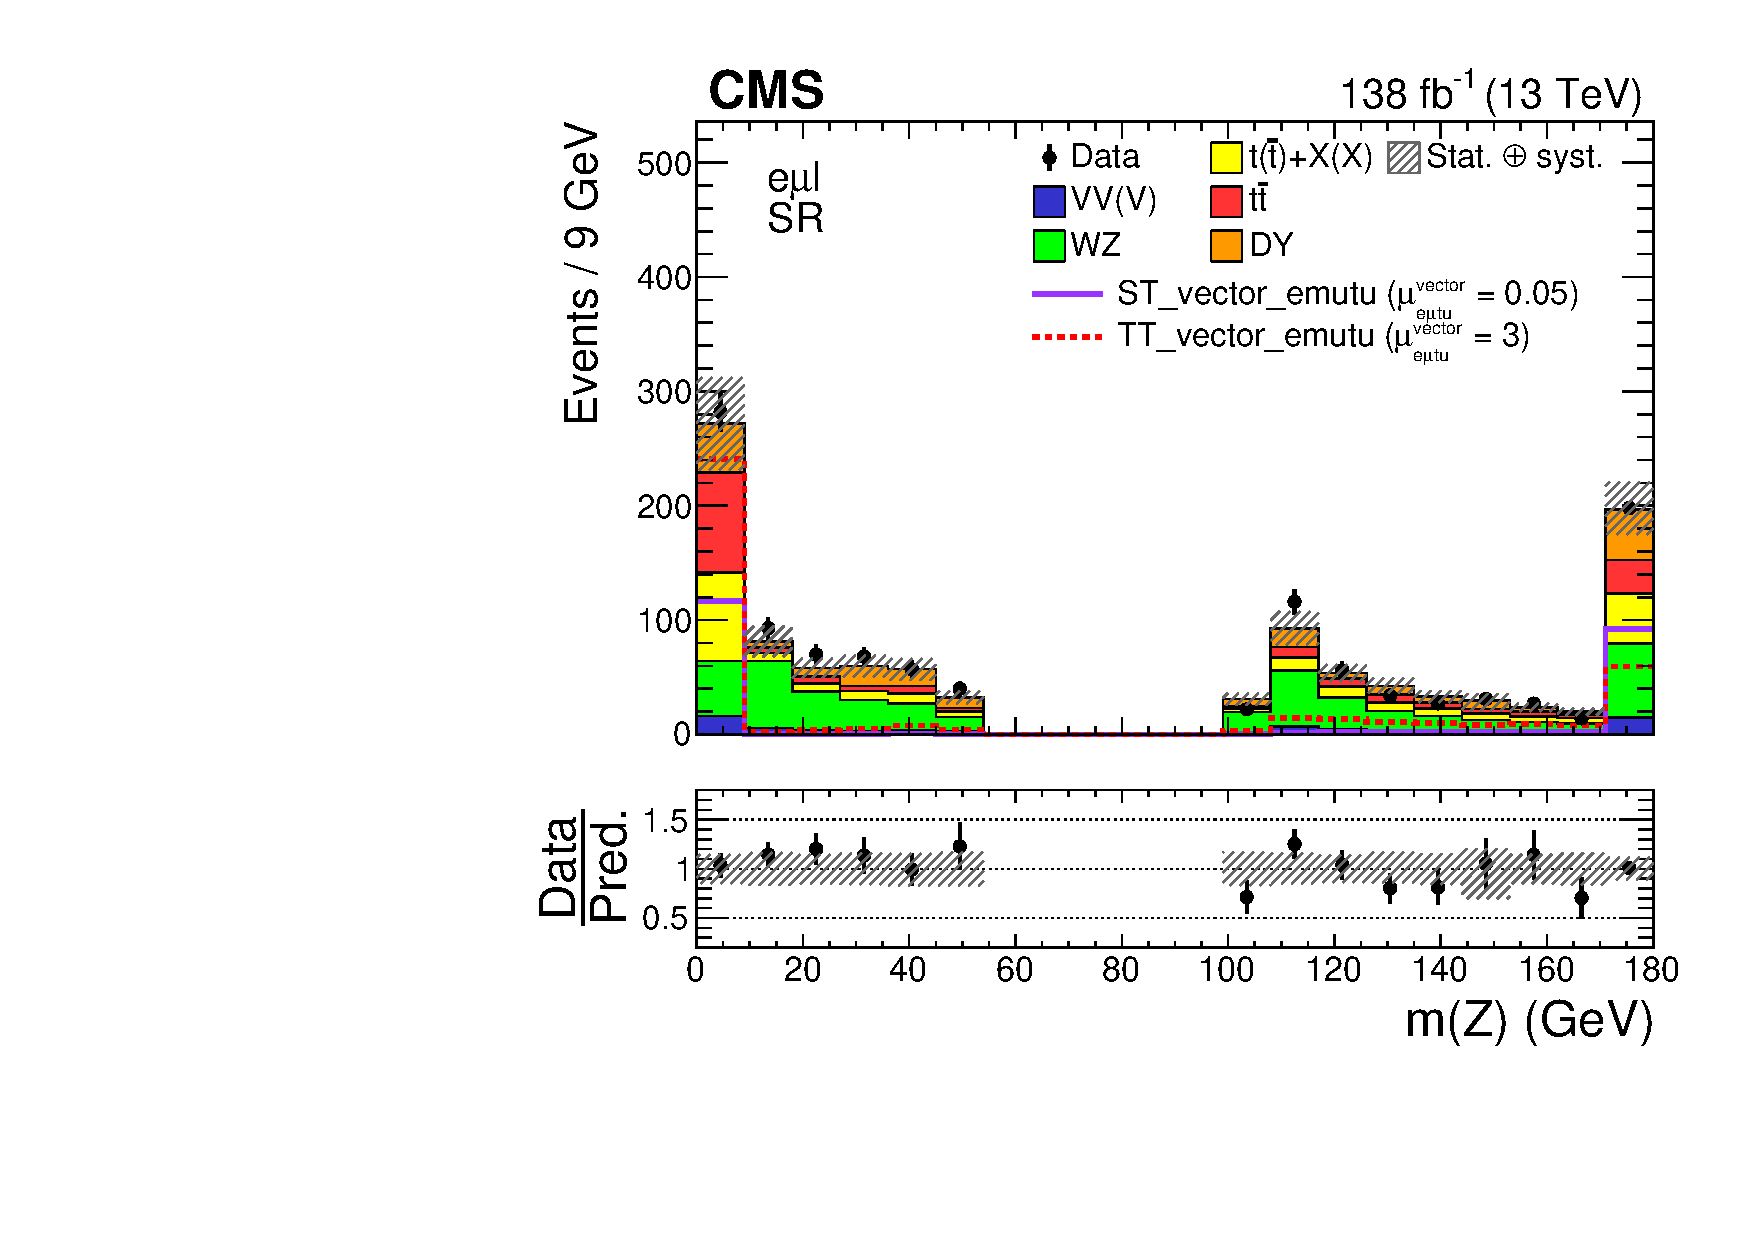
\includegraphics[width=0.48\textwidth]{figures/Part3/Selection/Zmass} \\
 \end{tabular}
 \caption{Distributions of the LFV e$\upmu$ mass (left) and the mass of the \ac{OSSF} lepton pair (right) in \ac{SR}. The data are shown as filled points and the \ac{SM} background predictions as histograms. The VV(V) background includes ZZ and triboson production, while the $\ttbar$ + X(X) component includes $\ttbar$W, $\ttbar$Z, $\ttbar$H, tZq, and smaller backgrounds containing one or two top quarks plus a boson or quark. All backgrounds are estimated using \ac{MC} simulation. The hatched bands indicate statistical and systematic uncertainties for the \ac{SM} background predictions. The normalization of the signal processes is chosen arbitrarily for improved visualization. The last bin of both histograms includes the overflow events.}
 \label{fig:SR}
 \end{center}
\end{figure}

Using the LFV e$\upmu$ mass, the \ac{SR} is further divided into two subsets to create top production and decay enriched regions:

\begin{itemize}
\item SR1, $\textsf{m}(\textsf{e}\upmu)~<$ 150 GeV: top quark decay enriched.
\item SR2, $\textsf{m}(\textsf{e}\upmu)~>$ 150 GeV: top quark production enriched.
\end{itemize}
%%%%%%%%%%%%%%%%%%%%%%%%%%%%%%%%%%%%%%%%%%%%%%%%%%%%%%%%%%%%%
%%%%%%%%%%%%%%%%%%%%%%%%%%%%%%%%%%%%%%%%%%%%%%%%%%%%%%%%%%%%%
\section{Validation Region}
\label{sec:VR}

\begin{figure}[tbh!]
 \begin{center}
 \begin{tabular}{c}
 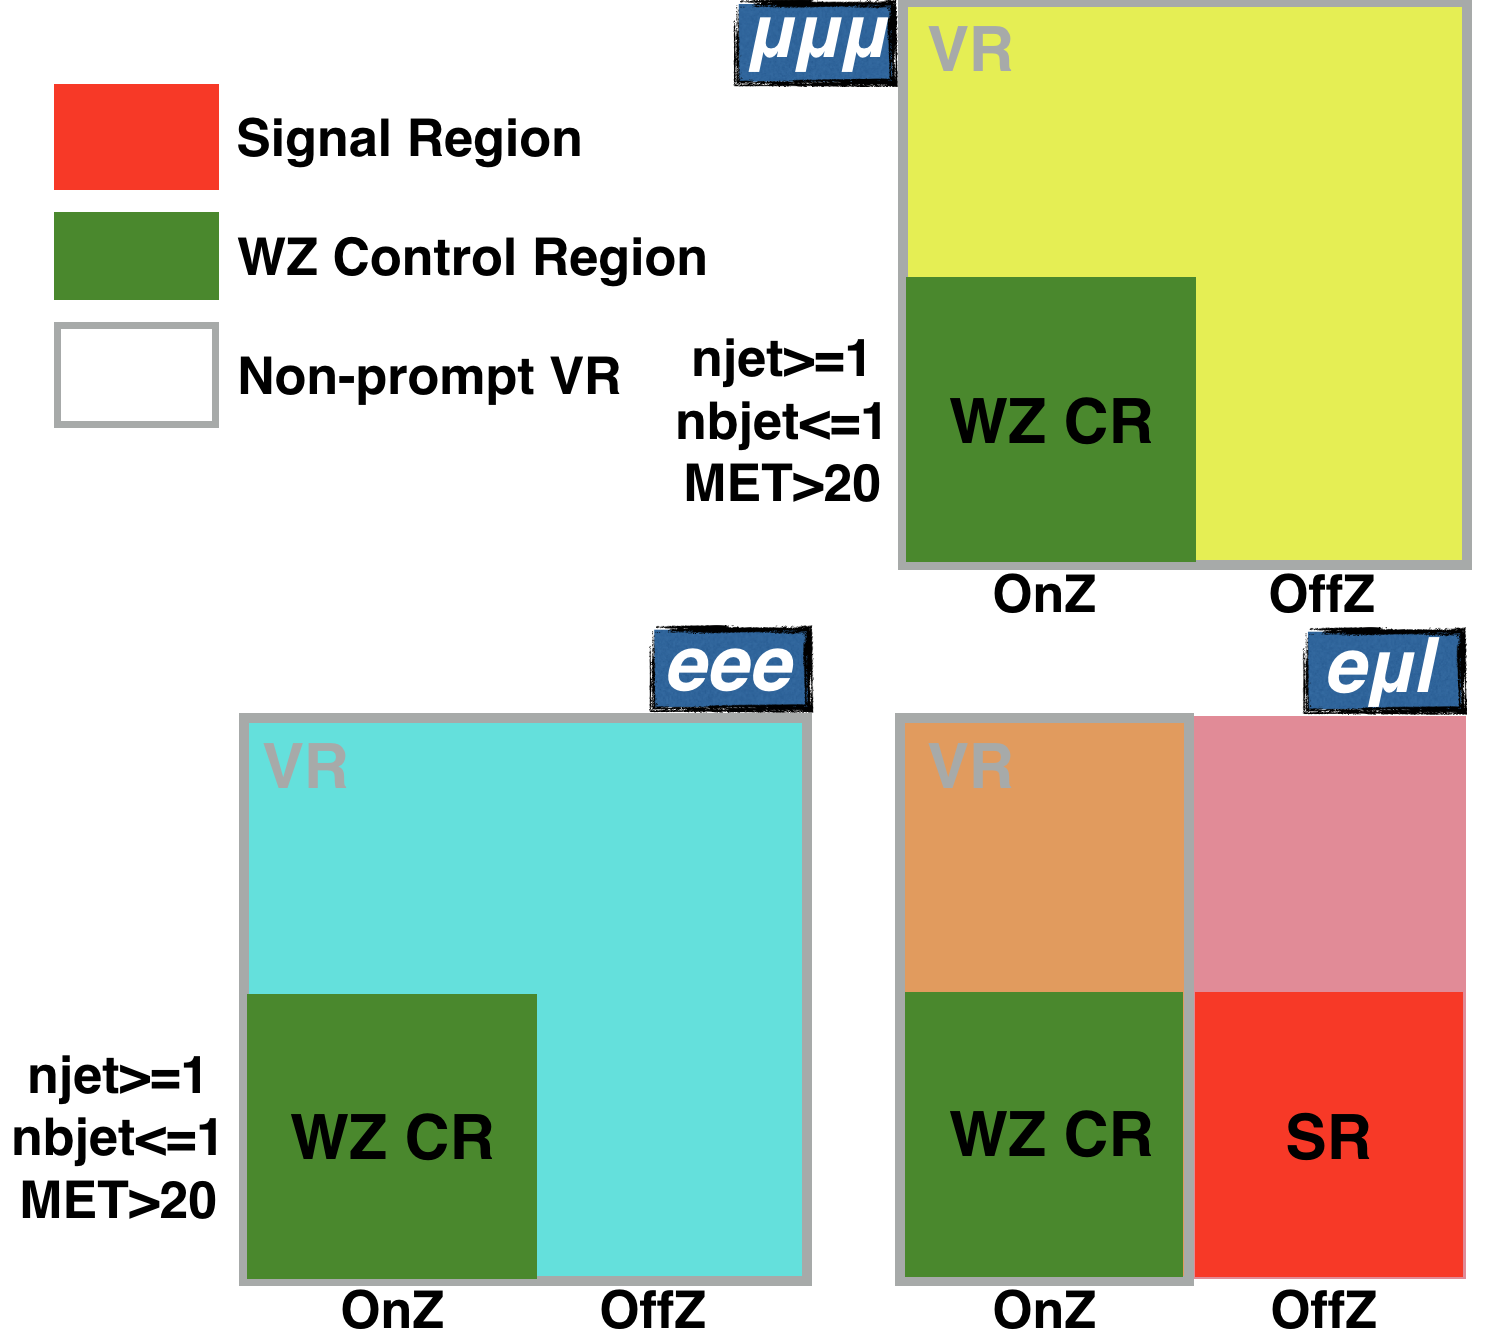
\includegraphics[width=0.8\textwidth]{figures/Part3/Selection/Event}
 \end{tabular}
 \caption{Illustration of selection criteria used to define different regions. ``OnZ'' means the presence of at least one \ac{OSSF} pair with an invariant mass between 50 GeV and 106 GeV. Events are labeled as ``OffZ'' when they fail ``OnZ'' criteria.}
 \label{fig:Event}
 \end{center}
\end{figure}

There are two types of signal-depleted \ac{VR} defined across three channels: \emph{nonprompt} \ac{VR} and WZ \ac{VR}. The purpose of these two types of \ac{VR} is only limited to the validation of the background modeling as neither of them enters the final fit. It is expected that the \emph{nonprompt} \ac{VR} has a significant fraction of \emph{nonprompt} background while WZ production is responsible for most of the backgrounds in the WZ \ac{VR}. Distributions of leading lepton $\pt$ and leading lepton $\eta$ in the WZ control region can be found in Figure~\ref{fig:WZ}. The \emph{nonprompt} \acp{VR} are further discussed in \autoref{chap:Nonprompt}.

Selection criteria used to define different regions are illustrated in Figure~\ref{fig:Event} and are summarized in Table~\ref{tab:region}.

\begin{figure}[tbh!]
 \begin{center}
 \begin{tabular}{cc}
 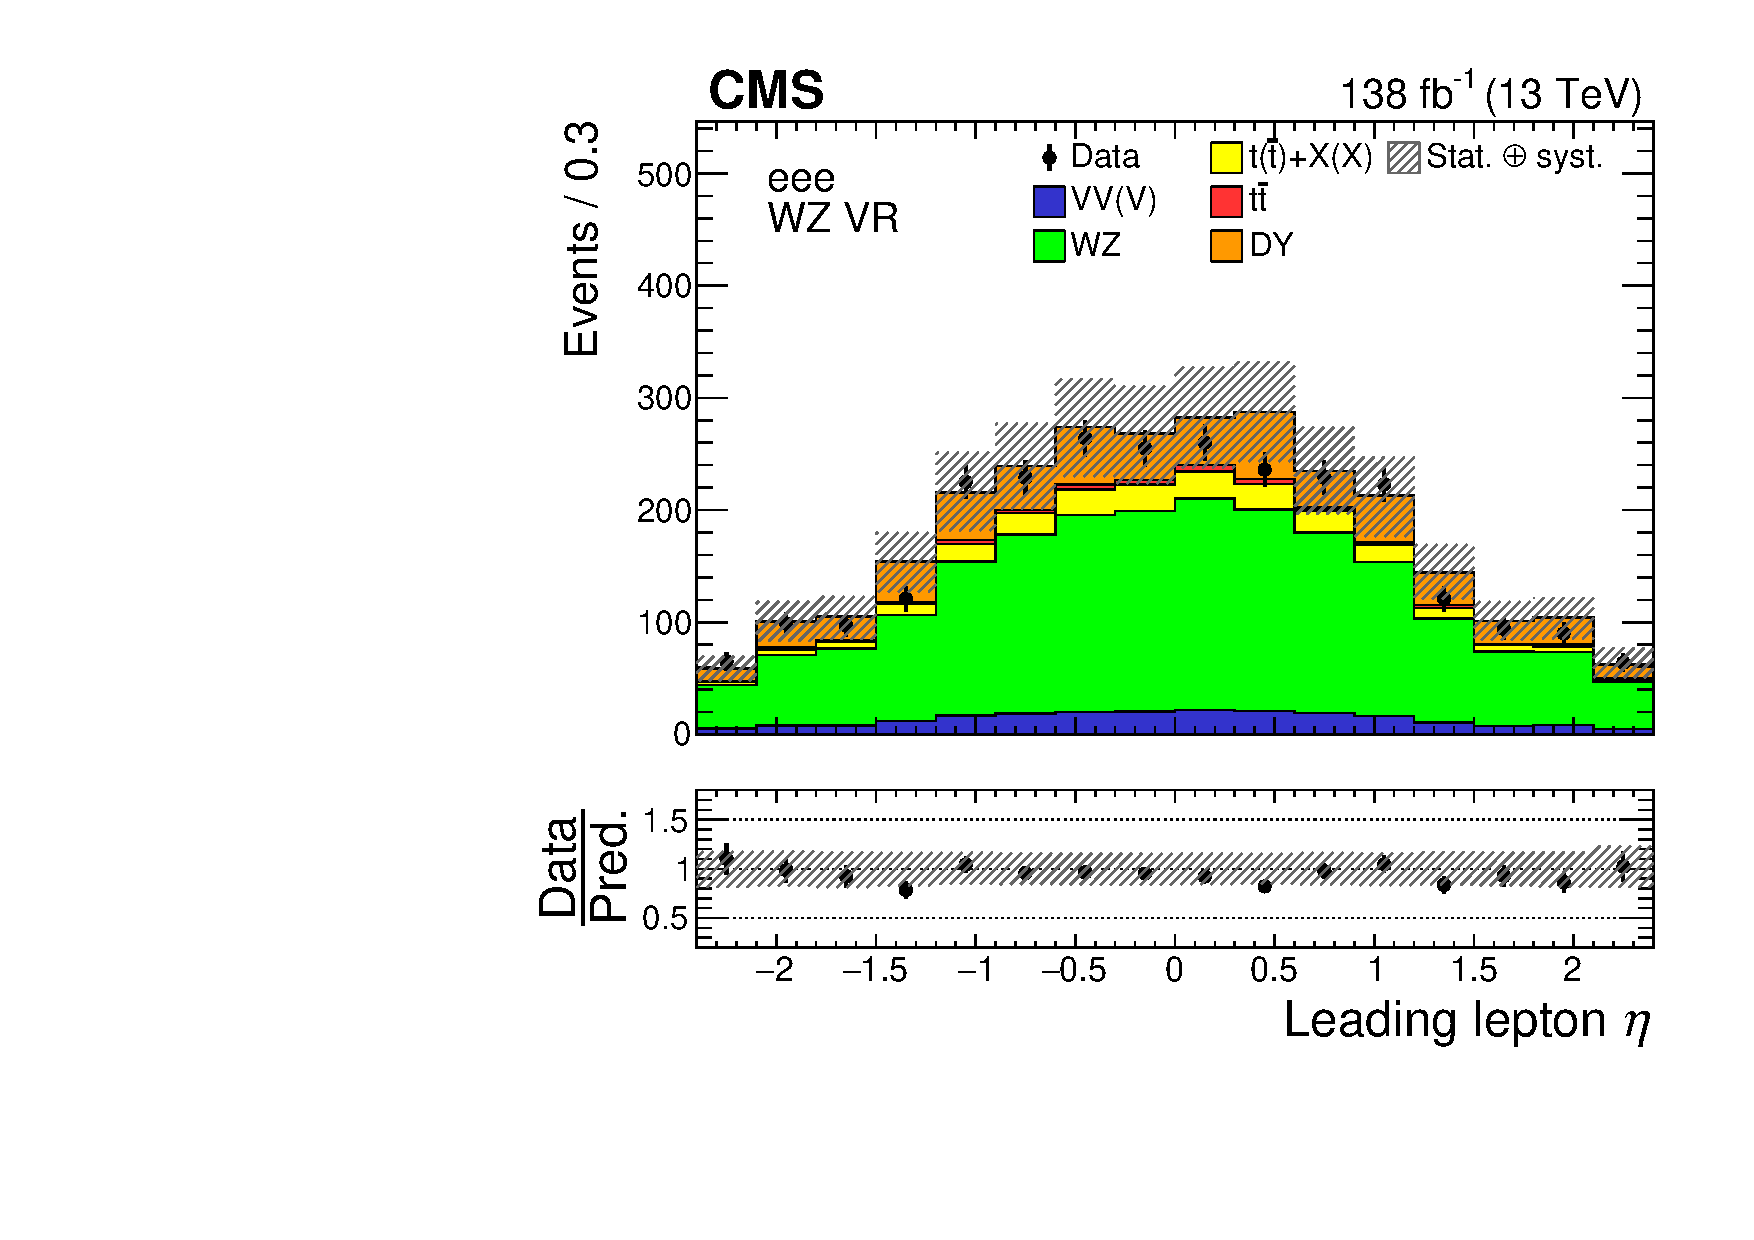
\includegraphics[width=0.48\textwidth]{figures/Part3/Selection/WZ/eee/lep1Eta}&
 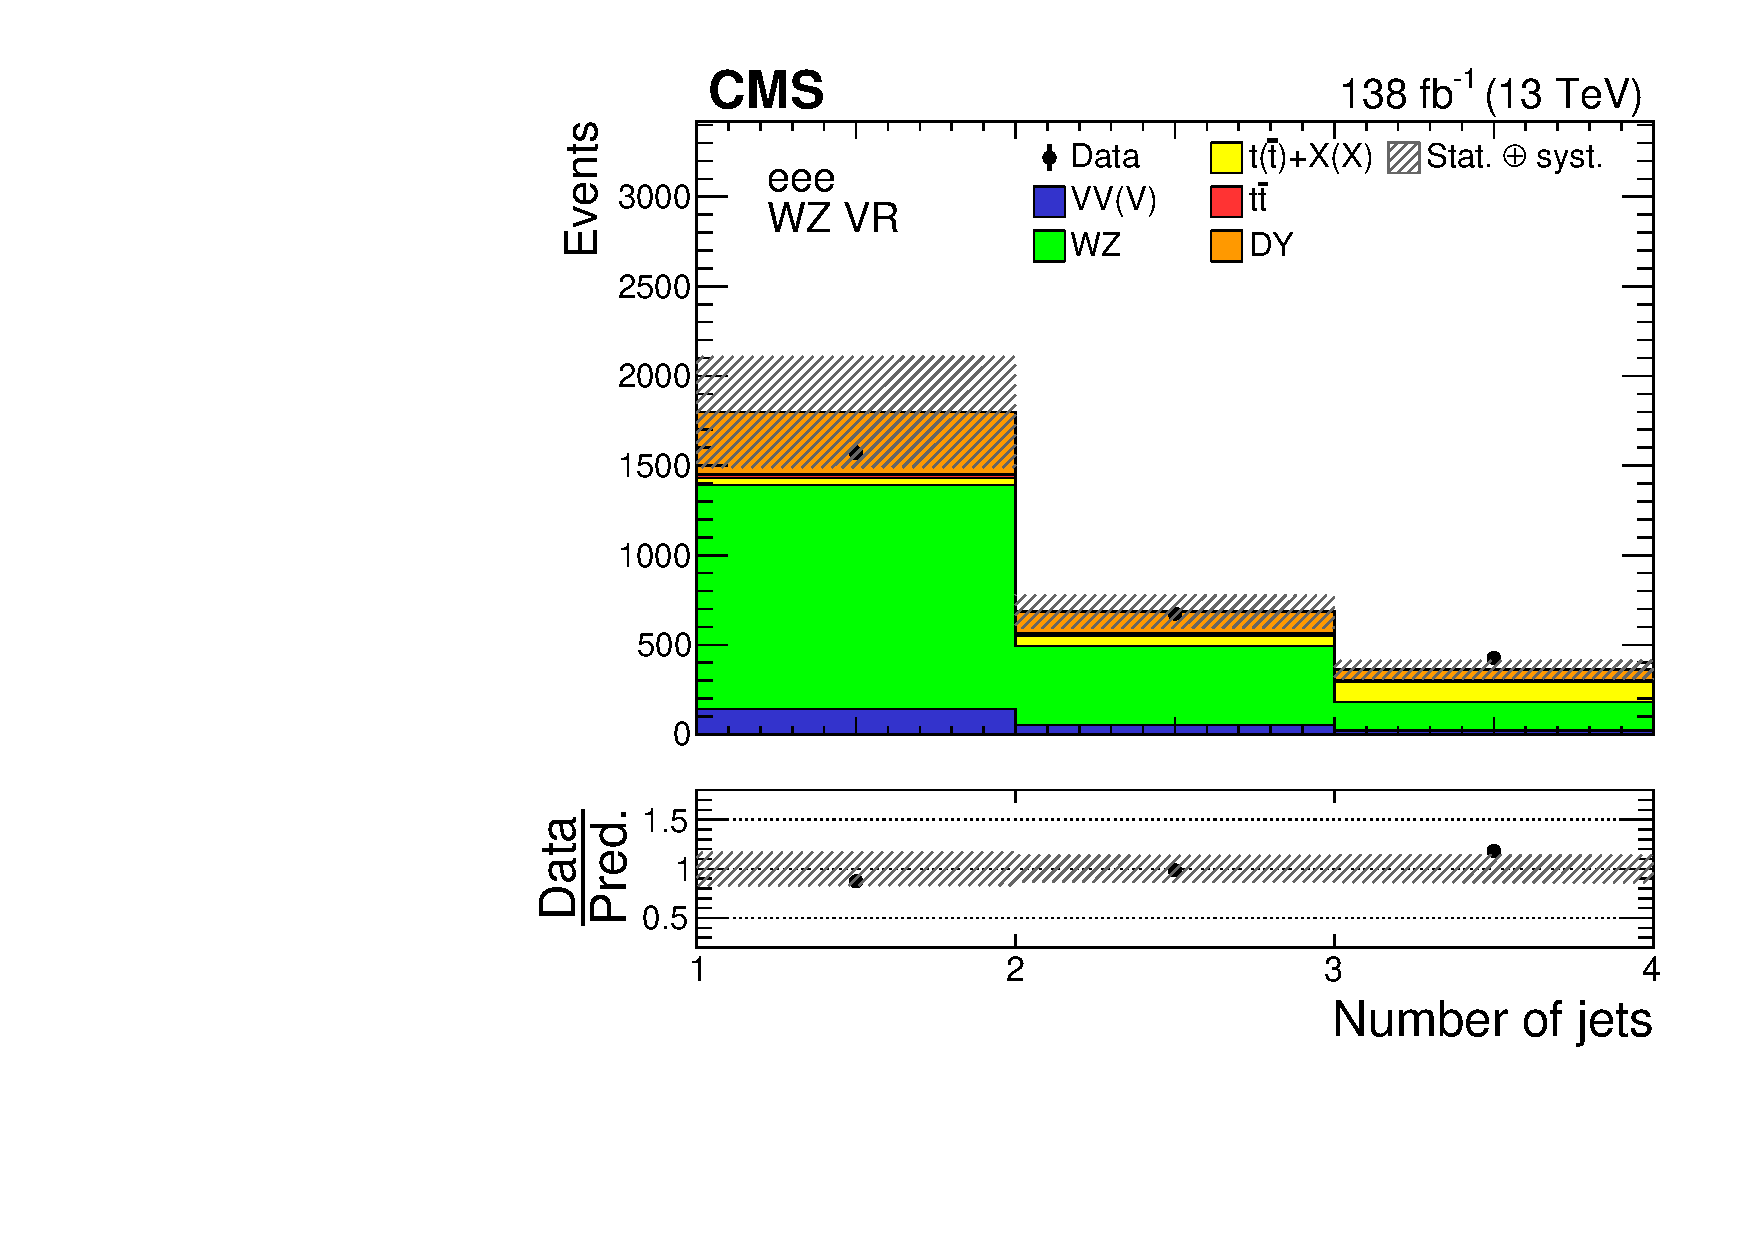
\includegraphics[width=0.48\textwidth]{figures/Part3/Selection/WZ/eee/njet} \\
 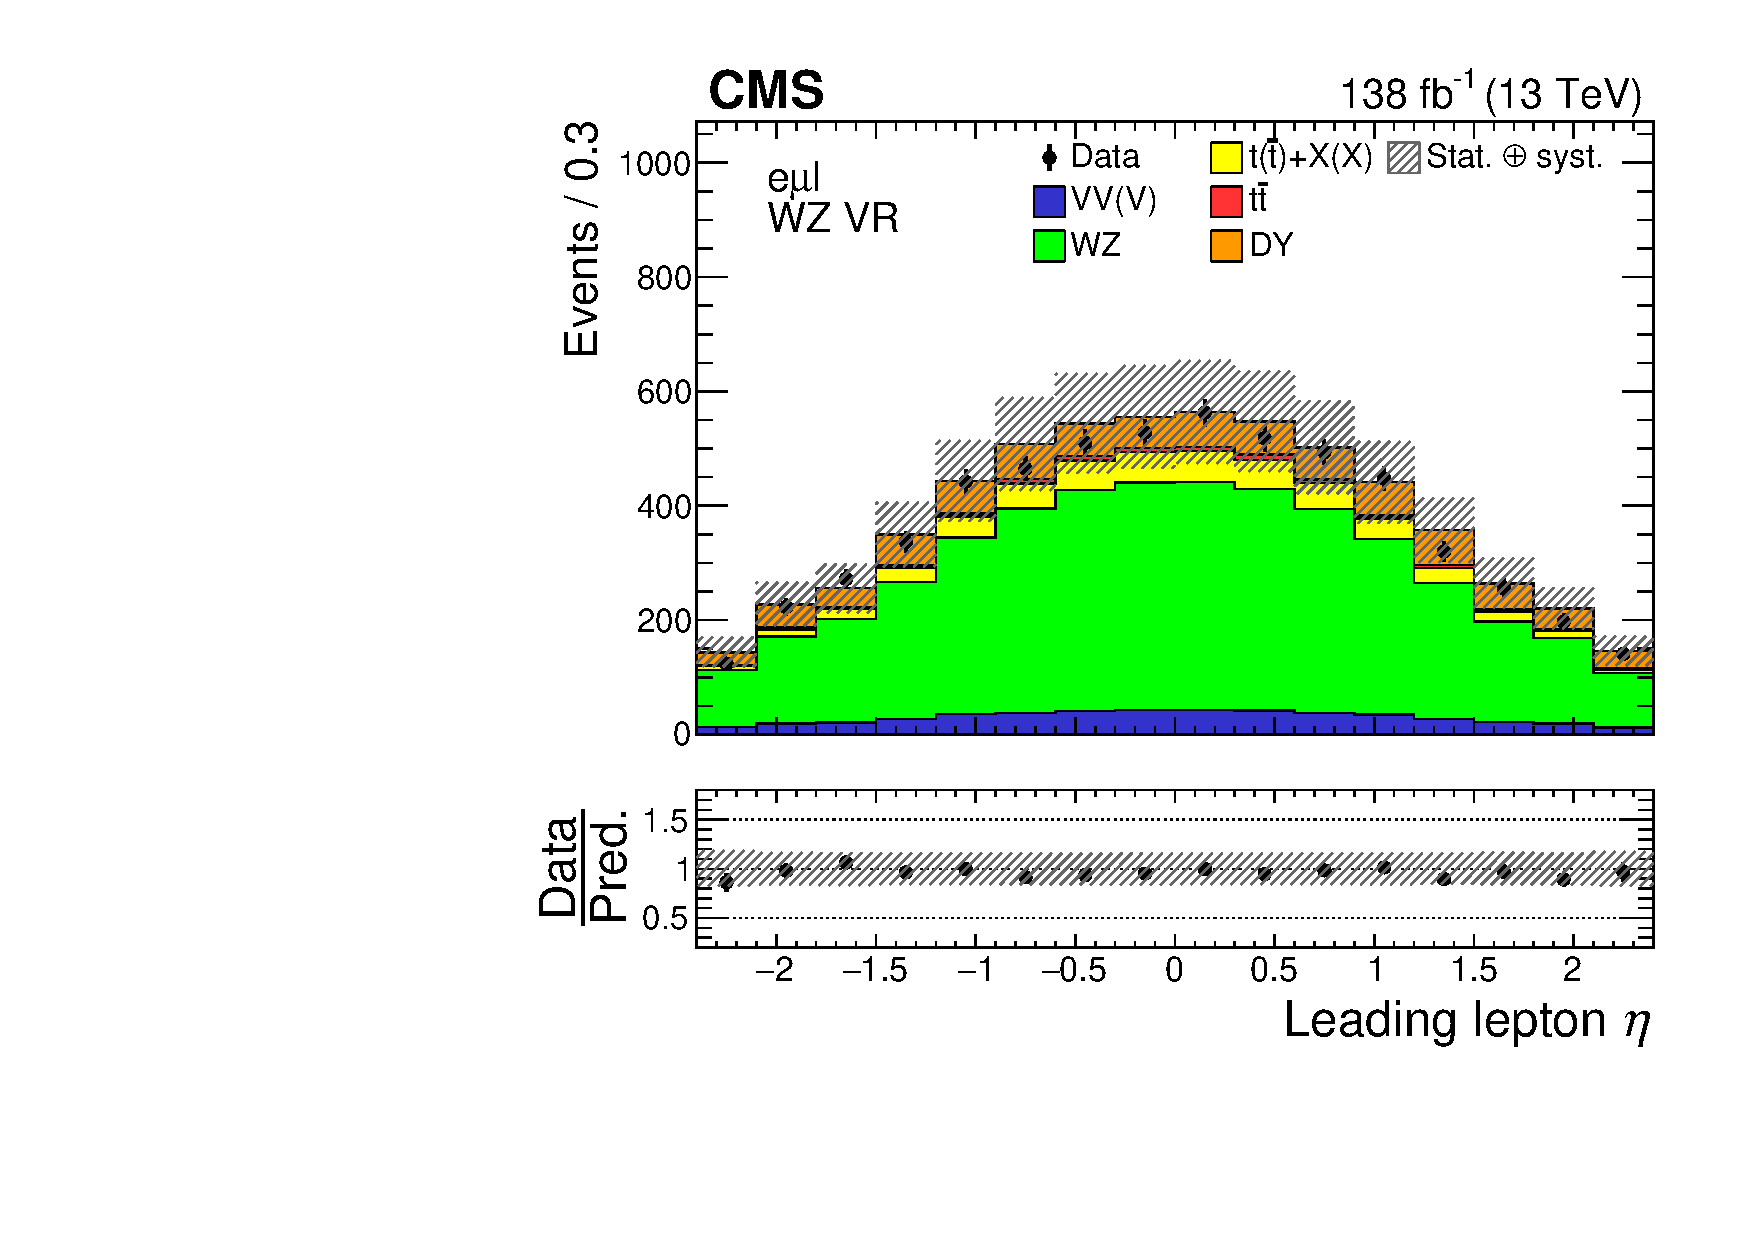
\includegraphics[width=0.48\textwidth]{figures/Part3/Selection/WZ/emul/lep1Eta}&
 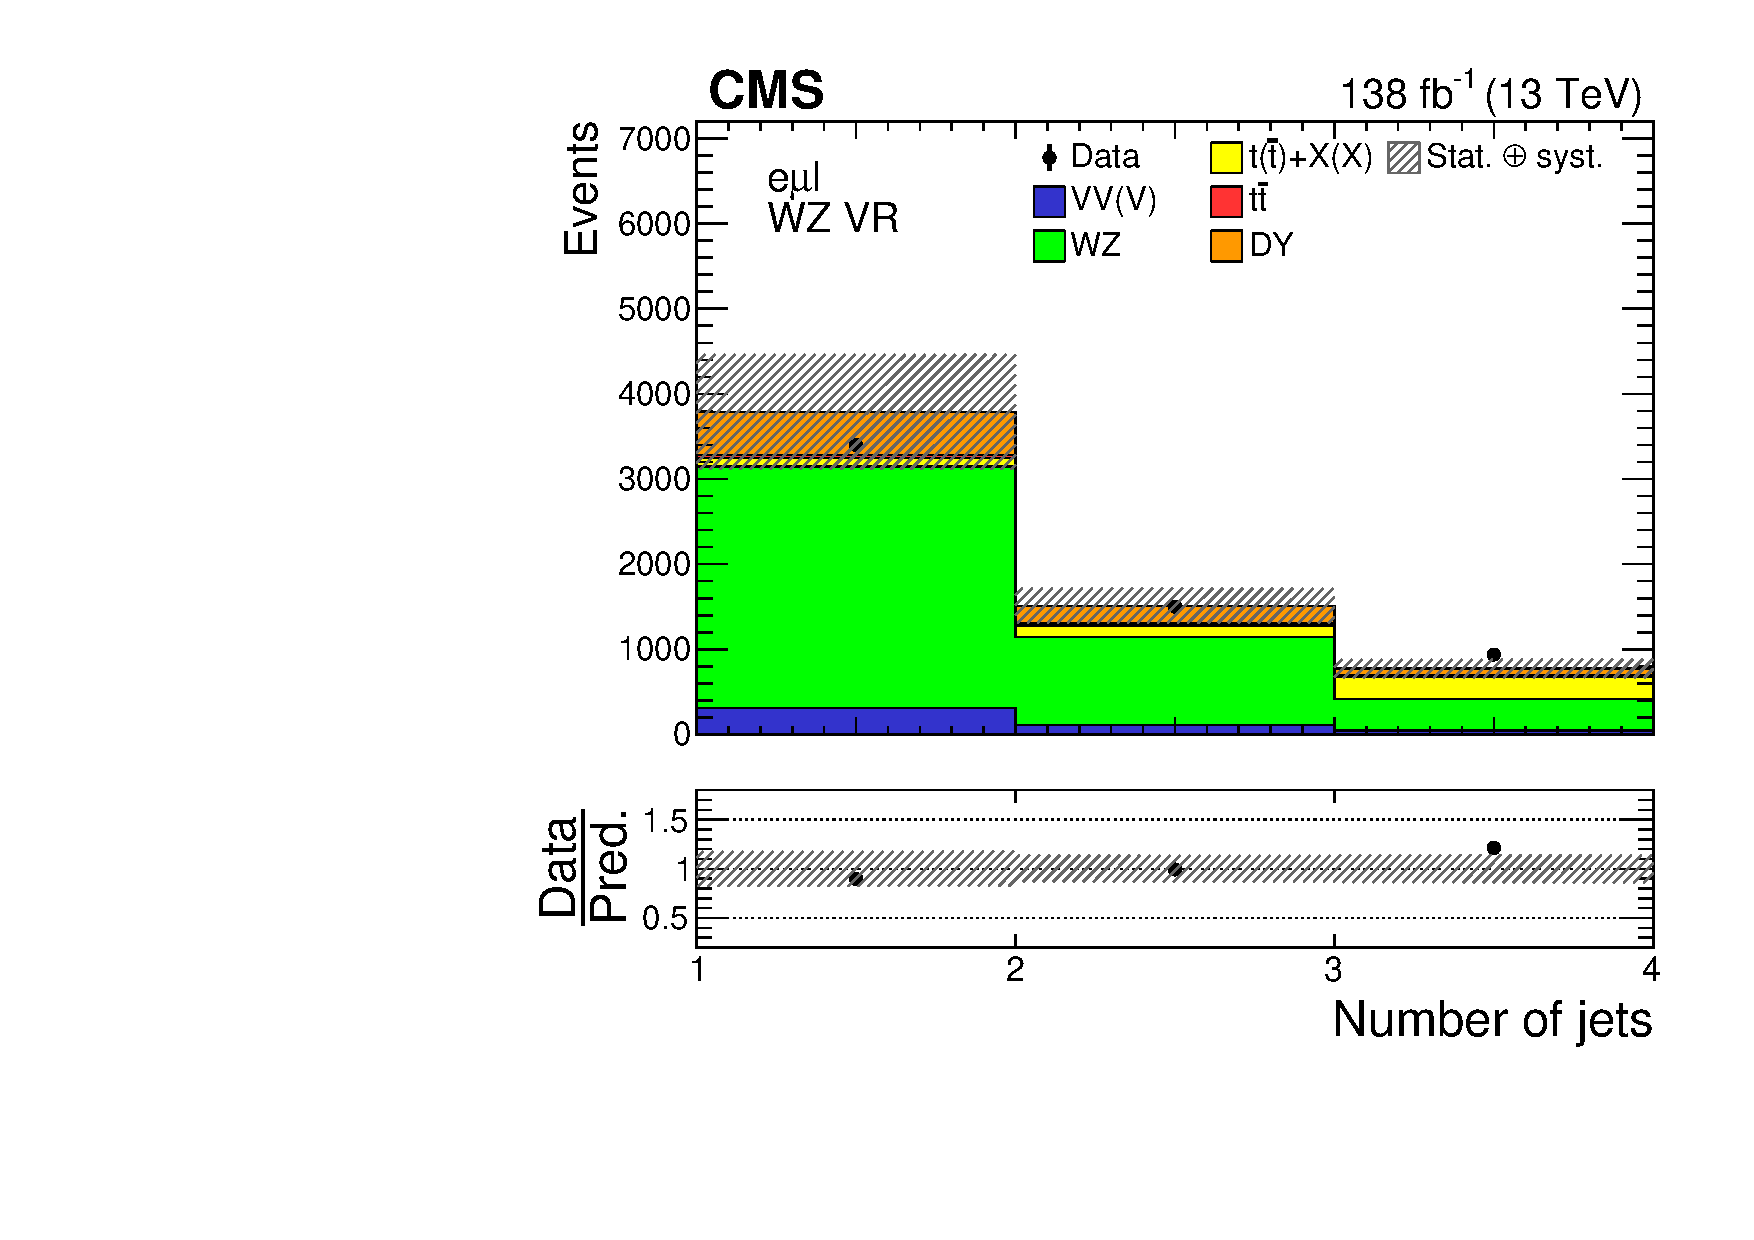
\includegraphics[width=0.48\textwidth]{figures/Part3/Selection/WZ/emul/njet} \\
 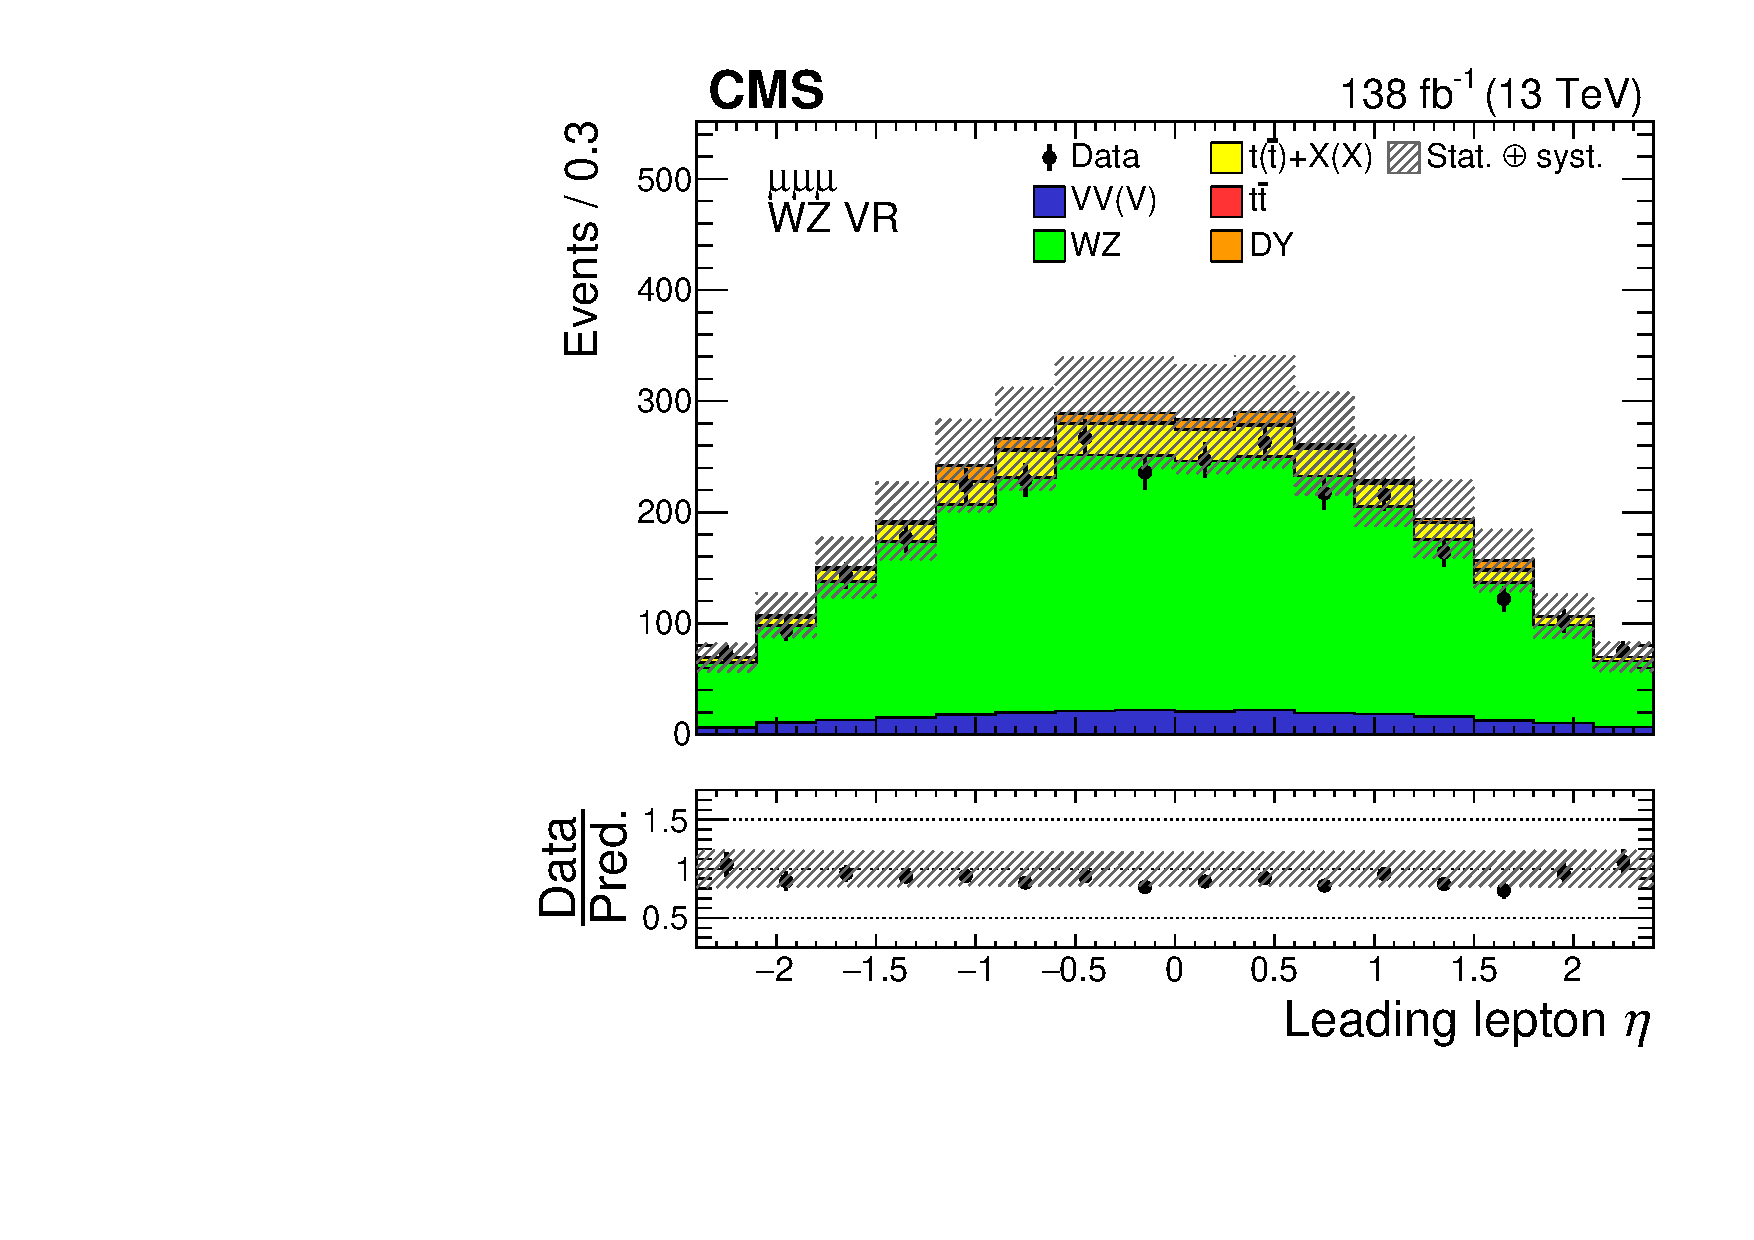
\includegraphics[width=0.48\textwidth]{figures/Part3/Selection/WZ/mumumu/lep1Eta}&
 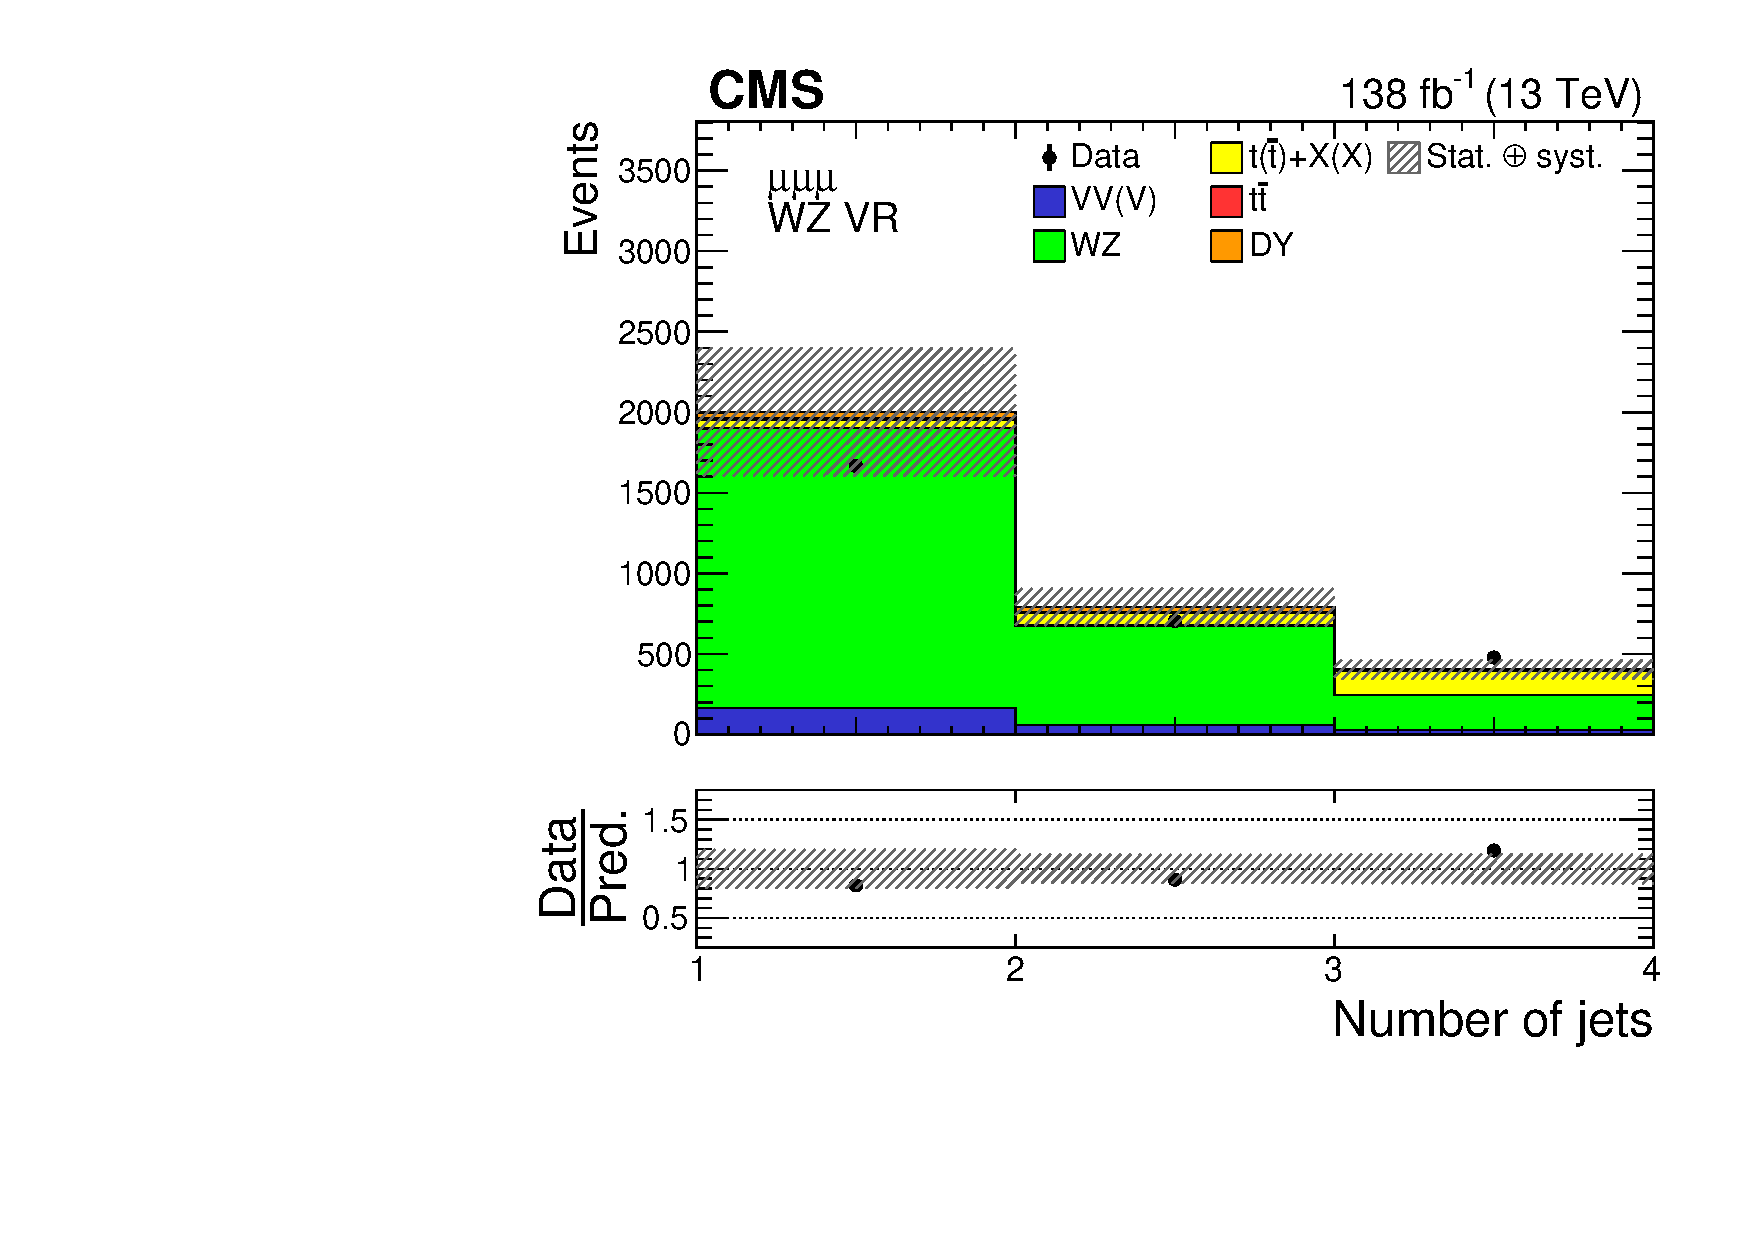
\includegraphics[width=0.48\textwidth]{figures/Part3/Selection/WZ/mumumu/njet} \\
 \end{tabular}
 \caption{Distributions of the leading lepton $\eta$ (left column) and the jet multiplicity (right column) in the WZ \acp{VR}. Events in the eee, $\emul$, and $\mmm$ WZ \acp{VR} are shown in the upper, middle, and lower rows, respectively. The data are shown as filled points and the background predictions as histograms. All backgrounds are estimated with \ac{MC} simulation. The hatched bands indicate statistical and systematic uncertainties for the background predictions. The last bin of the right column histograms includes the overflow events.}
 \label{fig:WZ}
 \end{center}
\end{figure}

\begin{table}[th]
\sffamily
\centering
\caption{Summary of the selection criteria used to define different event regions. ``OnZ'' means the presence of at least one \ac{OSSF} pair with an invariant mass between 50 GeV and 106 GeV. Events are labeled as ``OffZ'' when they fail ``OnZ'' criteria.}
\begin{tabular}{cccccccc}
\toprule
Channel   &Region & OnZ & OffZ & MET $>$ 20 GeV &njet$>=$1 &nbjet$<=$1\\ \midrule
\multirow{2}{*}{eee}  & VR & -  & -  & -  & -  & - \\  
   & WZ VR & \checkmark & -  & \checkmark & \checkmark & \checkmark\\ \midrule
\multirow{3}{*}{e$\upmu\ell$} & SR & -  & \checkmark & \checkmark & \checkmark & \checkmark \\
   & Nonprompt VR & \checkmark & -  & -  & -  & -  \\
   & WZ VR & \checkmark & -  & \checkmark & \checkmark & \checkmark \\ \midrule
\multirow{2}{*}{$\upmu\upmu\upmu$} & Nonprompt VR & -  & -  & -  & -  & -  \\  
   & WZ VR & -  & \checkmark & \checkmark & \checkmark & \checkmark \\ \bottomrule  
\end{tabular}
\label{tab:region}
\end{table}
%%%%%%%%%%%%%%%%%%%%%%%%%%%%%%%%%%%%%%%%%%%%%%%%%%%%%%%%%%%%%
%%%%%%%%%%%%%%%%%%%%%%%%%%%%%%%%%%%%%%%%%%%%%%%%%%%%%%%%%%%%%
\section{Kinematic Reconstruction}
\label{sec:Kin}

As mentioned, the LFV e$\upmu$ pair is assumed to be the product of the \ac{CLFV} interaction, while the third lepton, referred to as the standalone lepton, is assumed to originate from the leptonically decaying top quark. To distinguish this top quark (t$\rightarrow\ell\nu$b) from the top quark that decays via the \ac{CLFV} interaction (t$\rightarrow\textsf{e}\upmu$q), the former is referred to as the \ac{SM} top quark while the latter is referred to as the LFV top quark. 

The jet with the highest b-tagging score, regardless of whether or not it crosses the medium working point threshold, is assumed to originate from a bottom quark decay. Therefore, it is combined with \MET~to build the \ac{SM} top quark. The x and y components of \MET~are taken as measurements of neutrino $p_{\textsf{x}}$ and $p_{\textsf{y}}$. The z component of neutrino momentum is calculated by imposing the constraint that the invariant mass of the combined object (standalone lepton + neutrino) must be equal to W boson mass. If there is no real solution, the real part of the complex solution is taken. If there is more than one real solution, the solution that is the closest to the $p_{\textsf{z}}$ of the standalone lepton is taken. In events where there is more than one candidate of standalone lepton (i.e. the presence of the \ac{SSSF} pair), the lepton that gives a top mass that is the closest to the \ac{SM} top quark mass ($\mt$ = 172.5 GeV) is taken as the standalone lepton.

Once the standalone lepton has been determined, the remaining two leptons are labeled as the LFV e$\upmu$ pair and are combined with each selected jet to reconstruct the LFV top quark candidates. Jet with the highest b-tagging score is excluded from this reconstruction since it is assumed to be from the decay of the \ac{SM} top quark. Out of all the LFV top quark candidates, the candidate that gives a top mass that is the closest to the \ac{SM} top quark mass is taken. The LFV top quark mass is set to 0 in events where there are less than two jets.

A Z boson candidate is reconstructed using the \ac{OSSF} pair, which is not guaranteed to be present in the $\emul$ channel. The mass of the \ac{OSSF} lepton pair is set to 0 in events where the \ac{OSSF} is absent. The Z boson candidate is the only heavy particle reconstructed in the eee and $\mmm$ channels. Since there are always two ways to form the \ac{OSSF} pair, the \ac{OSSF} pair with an invariant mass that is closer to the Z boson mass ($\mz$ = 91.2 GeV) is taken. 

Jets with high b-tagging scores are combined with leptons to form so-called ``$\mbl$'' systems. The first $\mbl$ system takes the jet with the highest b-tagging score and combines it with each \emph{tight} lepton in events. Out of the three $\mbl$ system candidates, the one with the lowest $\mbl$ is taken, and the two constitutes are excluded from the consideration of the second $\mbl$ system. If additional jets exist, the second $\mbl$ system takes the jet with the highest b-tagging score and combines it with two of the remaining leptons separately. Out of the two candidates, the one with the lowest $\mbl$ is taken. $\mbl$ is set to 0 if no additional jet exists after the formation of the first $\mbl$ system.
\chapter{Nonprompt Background Estimation}
\label{chap:Nonprompt}

In this analysis, the term \emph{prompt} leptons refers to leptons that originate from the \ac{CLFV} vertex, the Drell-Yan process, or an electroweak boson decay, including leptons from $\uptau$ decays if the $\uptau$ lepton originates from the latter two processes. \emph{Nonprompt} leptons refer to leptons that originate from hadron decays and photon conversions, as well as particles misidentified as leptons. \emph{Nonprompt} leptons are suppressed through isolation requirements and a \ac{MVA}-based identification specifically trained to reject them.

\emph{Nonprompt} backgrounds are defined to be backgrounds with at least one \emph{nonprompt} lepton passing the \emph{tight} selection criteria, in this case generally dominated by Drell-Yan and $\ttbar$ production. An accurate estimation of \emph{nonprompt} backgrounds is difficult to achieve through \ac{MC} modelling. Therefore, a data-driven technique called the ``\mm'' \cite{Gillam:2014xua} is used to estimate the \emph{nonprompt} backgrounds. 

A brief description of the \mm~in its simplist form is given in \autoref{sec:MM} followed by its generalization and implementation in \autoref{sec:MR}. This method is validated using three \acp{VR} and is described in \autoref{sec:VR}. Lastly, the \emph{nonprompt} estimation in the \ac{SR} is presented in \autoref{sec:MMSR}.
%%%%%%%%%%%%%%%%%%%%%%%%%%%%%%%%%%%%%%%%%%%%%%%%%%%%%%%%%%%%
%%%%%%%%%%%%%%%%%%%%%%%%%%%%%%%%%%%%%%%%%%%%%%%%%%%%%%%%%%%%

\section{The Matrix Method}
\label{sec:MM}

The \mm~is a data driven technique used to estimate the fraction of \emph{nonprompt} leptons that pass a given lepton selection, referred to as ``\emph{tight}''. The \emph{tight} selection usually incorporates tight lepton identification and isolation requirements and corresponds to the full lepton selection used in an analysis. The \emph{loose} selection is obtained by loosening the \emph{tight} selection. The \emph{loose} selection is used as a baseline such that any \emph{loose} leptons fall into one of the two exclusive categories: \emph{tight} or \emph{not tight}. The \mm~deals with  \emph{prompt} and \emph{nonprompt} leptons separately. As a result, \emph{prompt} and \emph{nonprompt} efficiencies are introduced, as is illustrated in Figure~\ref{fig:Matrix_Method}.

 \begin{figure}[tbh!]
 \begin{center}
 \begin{tabular}{c}
 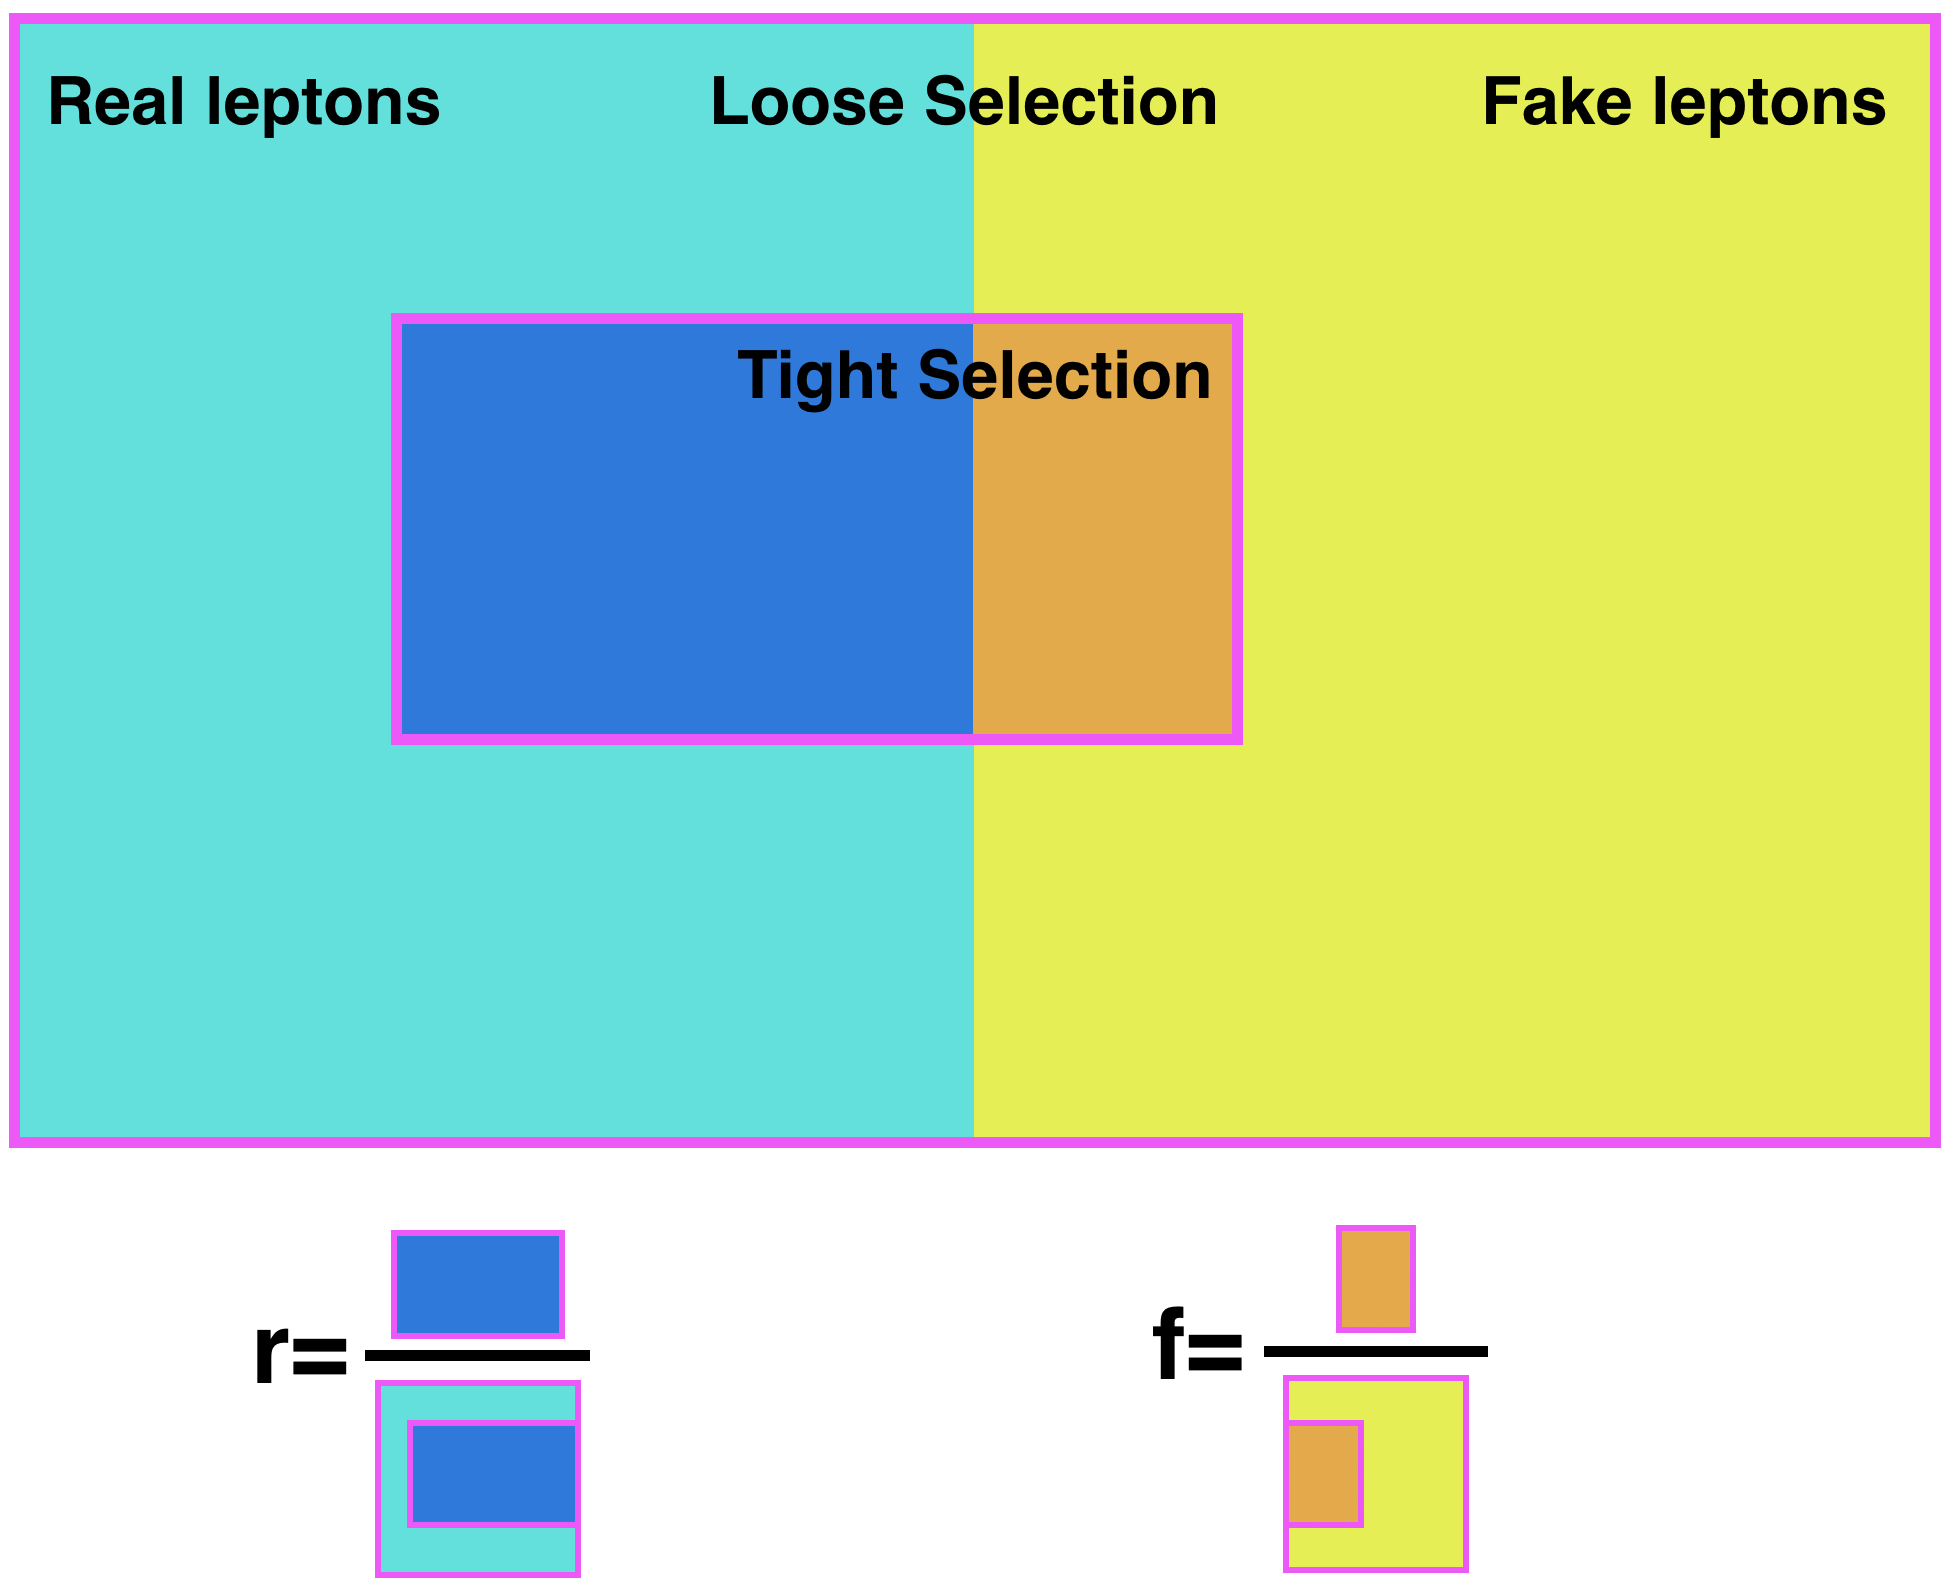
\includegraphics[width=0.8\textwidth]{figures/Part3/Nonprompt/matrix}
 \end{tabular}
 \caption{Illustration of the \emph{prompt} efficiency $r$ and the \emph{nonprompt} efficiency $f$.}
 \label{fig:Matrix_Method}
 \end{center}
\end{figure}

In a simplified scenario with only one lepton in the final state, the \emph{prompt} efficiency $r$ measures the probability of \emph{prompt} leptons pass \emph{tight} selection. It is treated as an observable that can be obtained through measurement,

\begin{equation}
r=\frac{n_P^{T}}{n_P^{T}+n_P^{\overline{T}}},
 \label{eq:real_rate}
\end{equation}
in which $n_P^{T}$/$n_P^{\overline{T}}$ denotes the number of events with a \emph{prompt} lepton that is \emph{tight}/\emph{not tight}.

Similarly, \emph{nonprompt} efficiency $f$ can be expressed as,

\begin{equation}
f=\frac{n_{N}^{T}}{n_{N}^{T}+n_{N}^{\overline{T}}},
 \label{eq:fake_rate}
\end{equation}
in which $n_{N}^{T}$/$n_{N}^{\overline{T}}$ denotes the number of events with a \emph{nonprompt} lepton that is \emph{tight}/\emph{not tight}.

The measurement of $r/f$ is often performed in dedicated control regions, where high purity of \emph{prompt}/\emph{nonprompt} leptons is expected. These regions are referred to as the \ac{MR}. It is assumed that $r/f$ is a universal property of \emph{prompt}/\emph{nonprompt} leptons that is independent of physics processes. Therefore, $r/f$ extracted from \ac{MR} can be used to estimate the contamination of \emph{nonprompt} leptons in a different region (e.g. \ac{SR}) even though these two regions are orthogonal to each other.

In this simplified scenario, the total number of events in the region of interest (e.g. \ac{SR}/\ac{VR}) with a \emph{tight}/\emph{not tight} lepton can be expressed in a system of equations,

\begin{equation}
\begin{split}
N^{T}&=N_{P}^{T}+N_{N}^{T}\\
N^{\overline{T}}&=N_{P}^{\overline{T}}+N_{N}^{\overline{T}},
\end{split}
\end{equation}

in which capital letter ``$N$'' is used to indicate that these numbers are referring to events in a region that is different from \ac{MR}. $N_{P}^{\overline{T}}$/$N_{N}^{\overline{T}}$ can be expressed in terms of $r/f$ and $N_{P}^{T}$/$N_{N}^{T}$ according to Equation \ref{eq:real_rate}/\ref{eq:fake_rate} and the assumption that r/f remains the same across different regions,

\begin{equation}
\begin{split}
N^{T}&=r\frac{N_{P}^{T}}{r}+f\frac{N_{N}^{T}}{f}\\
N^{\overline{T}}&=(1-r)\frac{N_{P}^{T}}{r}+(1-f)\frac{N_{N}^{T}}{f}.
\end{split}
\label{eq:sys_eq}
\end{equation}

Equation~\ref{eq:sys_eq} can also be expressed in the form of matrix,

\begin{equation}
 \begin{pmatrix}
 N^{T}\\
 N^{\overline{T}}
 \end{pmatrix}=\begin{pmatrix}
r&f\\
1-r&1-f
 \end{pmatrix}\begin{pmatrix}
 N_{P}^{T}/r\\
 N_{N}^{T}/f
 \end{pmatrix}.
 \label{eq:matrix}
 \end{equation}
 
Regions that correspond to the two numbers that appear in the righthand side vector of Equation~\ref{eq:matrix} are referred to as the ``\acp{AR}'', which can be constructed using experimental data. The estimation of \emph{nonprompt} background, denoted by $N_{N}^T$, can be obtained by a simple matrix inversion. 
%%%%%%%%%%%%%%%%%%%%%%%%%%%%%%%%%%%%%%%%%%%%%%%%%%%%%%%%%%%%
%%%%%%%%%%%%%%%%%%%%%%%%%%%%%%%%%%%%%%%%%%%%%%%%%%%%%%%%%%%%

\section{Generialization and Implementation of the  Matrix Method}
\label{sec:MR}

The description in previous section deals with a scenario where only one lepton is studied. This analysis uses a generalized version of the \mm, where all three \emph{tight} leptons are considered to be possibly \emph{nonprompt}. Equation~\ref{eq:matrix} is generalized as,

\begin{equation}
\hspace{-3.7em}
 \resizebox{1.2\linewidth}{!}{%
 $
 \begin{pmatrix}
 N^{TTT}\\\\
 N^{TT\overline{T}}\\\\
 N^{T\overline{T}T}\\\\
 N^{T\overline{T}\overline{T}}\\\\
 N^{\overline{T}TT}\\\\
 N^{\overline{T}T\overline{T}}\\\\
 N^{\overline{T}\overline{T}T}\\\\
 N^{\overline{T}\overline{T}\overline{T}}
 \end{pmatrix}=\begin{pmatrix}
r_1r_2r_3&r_1r_2f_3&r_1f_2r_3&r_1f_2f_3&f_1r_2r_3&f_1r_2f_3&f_1f_2r_3&f_1f_2f_3\\\\
r_1r_2(1-r_3)&r_1r_2(1-f_3)&r_1f_2(1-r_3)&r_1f_2(1-f_3)&f_1r_2(1-r_3)&f_1r_2(1-f_3)&f_1f_2(1-r_3)&f_1f_2(1-f_3)\\\\
r_1(1-r_2)r_3&r_1(1-r_2)f_3&r_1(1-f_2)r_3&r_1(1-f_2)f_3&f_1(1-r_2)r_3&f_1(1-r_2)f_3&f_1(1-f_2)r_3&f_1(1-f_2)f_3\\\\
r_1(1-r_2)(1-r_3)&r_1(1-r_2)(1-f_3)&r_1(1-f_2)(1-r_3)&r_1(1-f_2)(1-f_3)&f_1(1-r_2)(1-r_3)&f_1(1-r_2)(1-f_3)&f_1(1-f_2)(1-r_3)&f_1(1-f_2)(1-f_3)\\\\
(1-r_1)r_2r_3&(1-r_1)r_2f_3&(1-r_1)f_2r_3&(1-r_1)f_2f_3&(1-f_1)r_2r_3&(1-f_1)r_2f_3&(1-f_1)f_2r_3&(1-f_1)f_2f_3\\\\
(1-r_1)r_2(1-r_3)&(1-r_1)r_2(1-f_3)&(1-r_1)f_2(1-r_3)&(1-r_1)f_2(1-f_30&(1-f_1)r_2(1-r_3)&(1-f_1)r_2(1-f_3)&(1-f_1)f_2(1-r_3)&(1-f_1)f_2(1-f_3)\\\\
(1-r_1)(1-r_2)r_3&(1-r_1)(1-r_2)f_3&(1-r_1)(1-f_2)r_3&(1-r_1)(1-f_2)f_3&(1-f_1)(1-r_2)r_3&(1-f_1)(1-r_2)f_3&(1-f_1)(1-f_2)r_3&(1-f_1)(1-f_2)f_3\\\\
(1-r_1)(1-r_2)(1-r_3)&(1-r_1)(1-r_2)(1-f_3)&(1-r_1)(1-f_2)(1-r_3)&(1-r_1)(1-f_2)(1-f_3)&(1-f_1)(1-r_2)(1-r_3)&(1-f_1)(1-r_2)(1-f_3)&(1-f_1)(1-f_2)(1-r_3)&(1-f_1)(1-f_2)(1-f_3)
 \end{pmatrix}\begin{pmatrix}
 N_{PPP}^{TTT}/r_1r_2r_3\\\\
 N_{PPN}^{TTT}/r_1r_2f_3\\\\
 N_{PNP}^{TTT}/r_1f_2r_3\\\\  
 N_{PNN}^{TTT}/r_1f_2f_3\\\\
 N_{NPP}^{TTT}/f_1r_2r_3\\\\
 N_{NPN}^{TTT}/f_1r_2f_3\\\\
 N_{NNP}^{TTT}/f_1f_2r_3\\\\
 N_{NNN}^{TTT}/f_1f_2f_3
 \end{pmatrix}.
 $}
 \label{eq:matrix_method3}
 \end{equation}
 
All but the first number that appear in the righthand side vector correspond to events with at least one \emph{nonprompt} lepton that pass \emph{tight} selection criteria. Therefore, the overall \emph{nonprompt} background is expresses as,
 
\begin{equation}
N_{Nonprompt}^{TTT} = N_{PPN}^{TTT} + N_{PNP}^{TTT} + N_{PNN}^{TTT} + N_{NPP}^{TTT} + N_{NPN}^{TTT} + N_{NNP}^{TTT} + N_{NNN}^{TTT},
\end{equation}
 
which can be obtained by first constructing 8 \acp{AR} to form the lefthand side vector. Secondly, the 8 $\times$ 8 matrix is constructed and inverted. Lastly, the righthand side vector can be obtained by multiplying the lefthand side vector to the inverted matrix.

Only two \acp{PD} ``SingleElectron'' and ``SingleMuon'' are used in the construction of \ac{MR} in 2016 and 2017 while ``SingleElectron'' is replaced with ``EGamma'' in 2018. In addition to \acp{PD}, the measurements of $r$/$f$ also utilize the $\ttbar$ sample and all \ac{MC} samples listed under the ``\emph{prompt} background'' category in Table~\ref{tab:MCsample}. Depending on the flavor of the leading lepton in \ac{MC}, events are selected with either a single-electron or a single-muon trigger, which is summarized in Table~\ref{tab:RandF_trigger}. Data events are selected with the same \ac{HLT} triggers as well but events in ``SingleMuon'' (``SingleElectron'' or ``EGamma'') \ac{PD} are only accepted if the leading lepton is a muon (electron).

\begin{table}[th]
\sffamily
\centering
\begin{tabular}{llllll}
\toprule
Channel   & Path       & Dataset  & 2016 & 2017 & 2018 \\ \midrule
\multirow{2}{*}{Electron} & HLT\_Ele27\_WPTight\_Gsf  & Data \& MC & \checkmark & - & - \\ 
           & HLT\_Ele35\_WPTight\_Gsf & Data \& MC & - & \checkmark & \checkmark \\ \hline
\multirow{1}{*}{Muon}  & HLT\_IsoMu27 & Data \& MC & \checkmark & \checkmark & \checkmark \\ \bottomrule
\end{tabular}
\caption{Summary of the \ac{HLT} triggers used in the measurement of $r$ and $f$.}
\label{tab:RandF_trigger}
\end{table}

Both $r$ and $f$ are parameterized in bins of lepton $\pt$, $|\eta|$, and jet multiplicity. The bin range is optimized to retain sufficient statistics for each bin:

\begin{itemize}
\item Electron $\pt$ bin range: \{20.0, 24.6, 28.8, 33.0, 37.2, 41.4, 46.1, 52.1, 59.3, 68.3, 82.7, 110.6\} GeV,
\item Muon $\pt$ bin range: \{20.0, 23.8, 27.7, 31.3, 35.0, 38.9, 42.8, 45.6, 50.7, 59.5, 72.9, 94.3\} GeV,
\item $|\eta|$ bin range: \{0, 0.8, 1.6, 2.4\},
\item Jet multiplicity: \{0 jet, $\geq$ 1 jet\}.
\end{itemize}

The jet multiplicity bin is a proxy for variation of the composition of physics processes. In addition to requiring at least one jet, the \ac{MR} corresponds to the second jet multiplicity bin requires no more than one b-tagged jet as this is also required in the \ac{SR}.

The \emph{nonprompt} efficiency is measured in same-sign dilepton regions, in which the leading lepton in $\pt$, used as a \emph{tag}, is required to be matched with trigger objects within $\mathrm{\Delta}R~<$ 0.2. The sub-leading lepton is required to pass the \emph{loose} selection and is taken as the \emph{probe}. Events that have two same-sign electrons with an invariant mass between 76 GeV and 106 GeV are removed from \ac{MR} to suppress the backgrounds that originate from charge misidentification. No such requirement has been introduced to the muon \ac{MR} due to its negligible rate of  charge misidentification.

The contribution from \emph{prompt} backgrounds, estimated from \ac{MC} simulation, are subtracted from data. A representative composition of backgrounds in \ac{MR} is shown in Figure~\ref{fig:MRexample}. 

\begin{figure}[tbh!]
 \begin{center}
 \begin{tabular}{cc}
 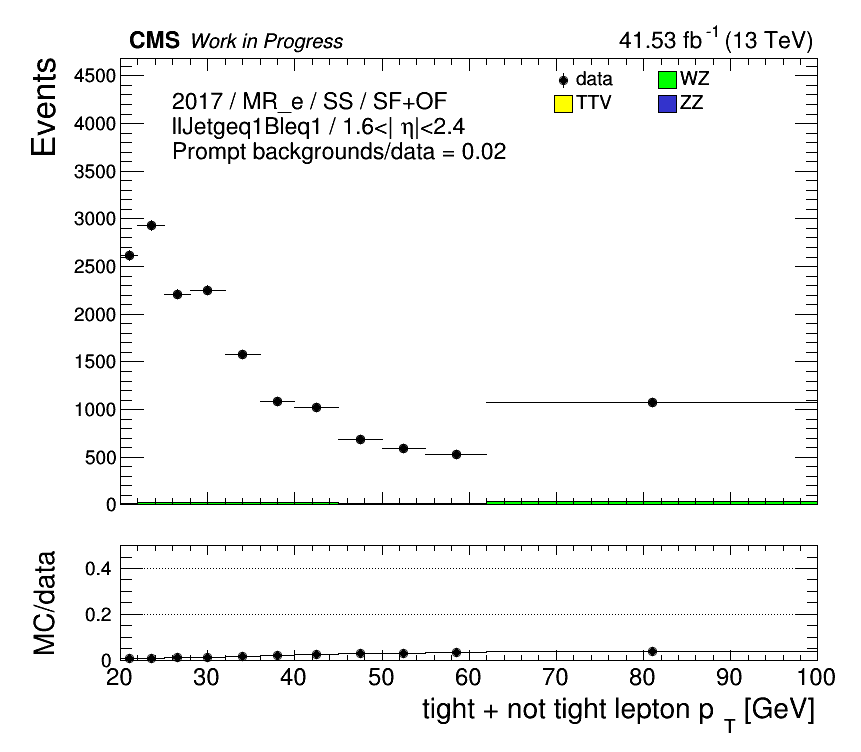
\includegraphics[width=0.45\textwidth]{figures/Part3/Nonprompt/MR/FlepPt}&
 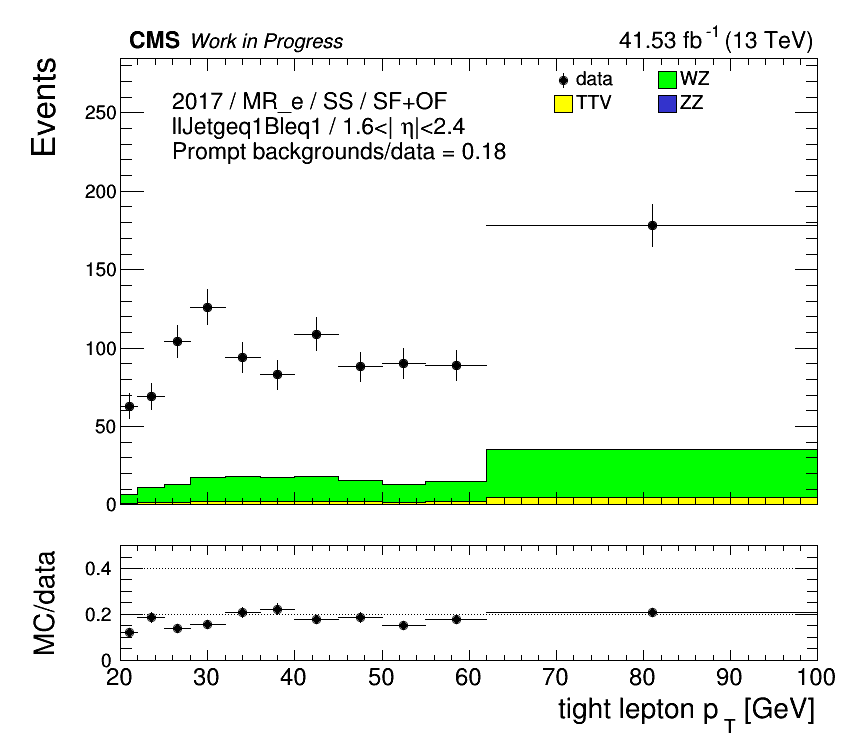
\includegraphics[width=0.45\textwidth]{figures/Part3/Nonprompt/MR/TlepPt} \\
 \end{tabular}
 \caption{Distribution of lepton $\pt$ in a representative electron \emph{nonprompt} efficiency \ac{MR}. In this particular example, both ee and $\upmu$e flavor composites are considered. At least one jet and at most one b-tagged jet are required (the second jet multiplicity bin). \emph{Probe} electron is required to have $1.6<|\eta|<2.4$ (the third $\eta$ bin). Contamination from \emph{prompt} backgrounds are estimated with \ac{MC} simulation, and are shown as histograms. The data are shown as filled points. From left to right: \emph{loose} (i.e. \emph{tight + not tight}) electron $\pt$, \emph{tight} electron $\pt$.}
 \label{fig:MRexample}
 \end{center}
\end{figure}

The fake efficiency $f$ is calculated as:

\begin{equation}
f=\frac{n_{data}^{tag+tight}-n_{MC(prompt)}^{tag+tight}}{n_{data}^{tag+loose}-n_{MC(prompt)}^{tag+loose}},
\label{eq:f_eq}
\end{equation}  

where the numerator is selected with one \emph{tag} and one \emph{tight} lepton while the denominator is selected with one \emph{tag} and one \emph{loose} lepton. The selection criteria for \emph{tag}, \emph{loose}, and \emph{tight} lepton is summarised in Table~\ref{tab:MR}.

\begin{table}[th]
\sffamily
\centering
\begin{tabular}{ccccc}
\toprule
Lepton   &Selection   & \emph{loose} & \emph{tag} & \emph{tight}$^{\textsf{ii}}$\\ \midrule
\multirow{4}{*}{Electron} & $\pt$  & $>$ 20 GeV & $>$ 38 GeV$^{\textsf{i}}$ & $>$ 20 GeV \\  
     & $I_{\textsf{mini}}^{\textsf{rel}}$  & $<$0.4 & $<$0.1 & $<$0.12 \\
     & \TOP   & $>$-0.9   & $>$0.95 & $>$0.9 \\ 
     & Match with trigger objects   & - & \checkmark & -  \\ \midrule
\multirow{5}{*}{Muon} & $\pt$ & $>$ 20 GeV & $>$ 30 GeV & $>$ 20 GeV \\
     & $I_{\textsf{mini}}^{\textsf{rel}}$  & $<$0.4 & $<$0.1 & $<$0.12 \\
     & Cut-based ID  & - & Medium WP & Medium WP \\
     & \TOP   & $>$0.5 & $>$0.9 & $>$0.9 \\ 
     & Match with trigger objects   & - & \checkmark & -  \\ \bottomrule
\end{tabular}
\caption{Summary of the lepton selections needed for the measurement of $r$ and $f$. Please note: (i) the minimum $\pt$ cut for \emph{tag} electron in 2016 dataset is reduced to 30 GeV to adjust for the trigger threshold, and (ii) the \emph{tight} selection here is the same as the \emph{tight} lepton selection described in \autoref{sec:Leptons}.}
\label{tab:looseandtight}
\end{table}

\begin{figure}[tbh!]
 \begin{center}
 \begin{tabular}{c}
 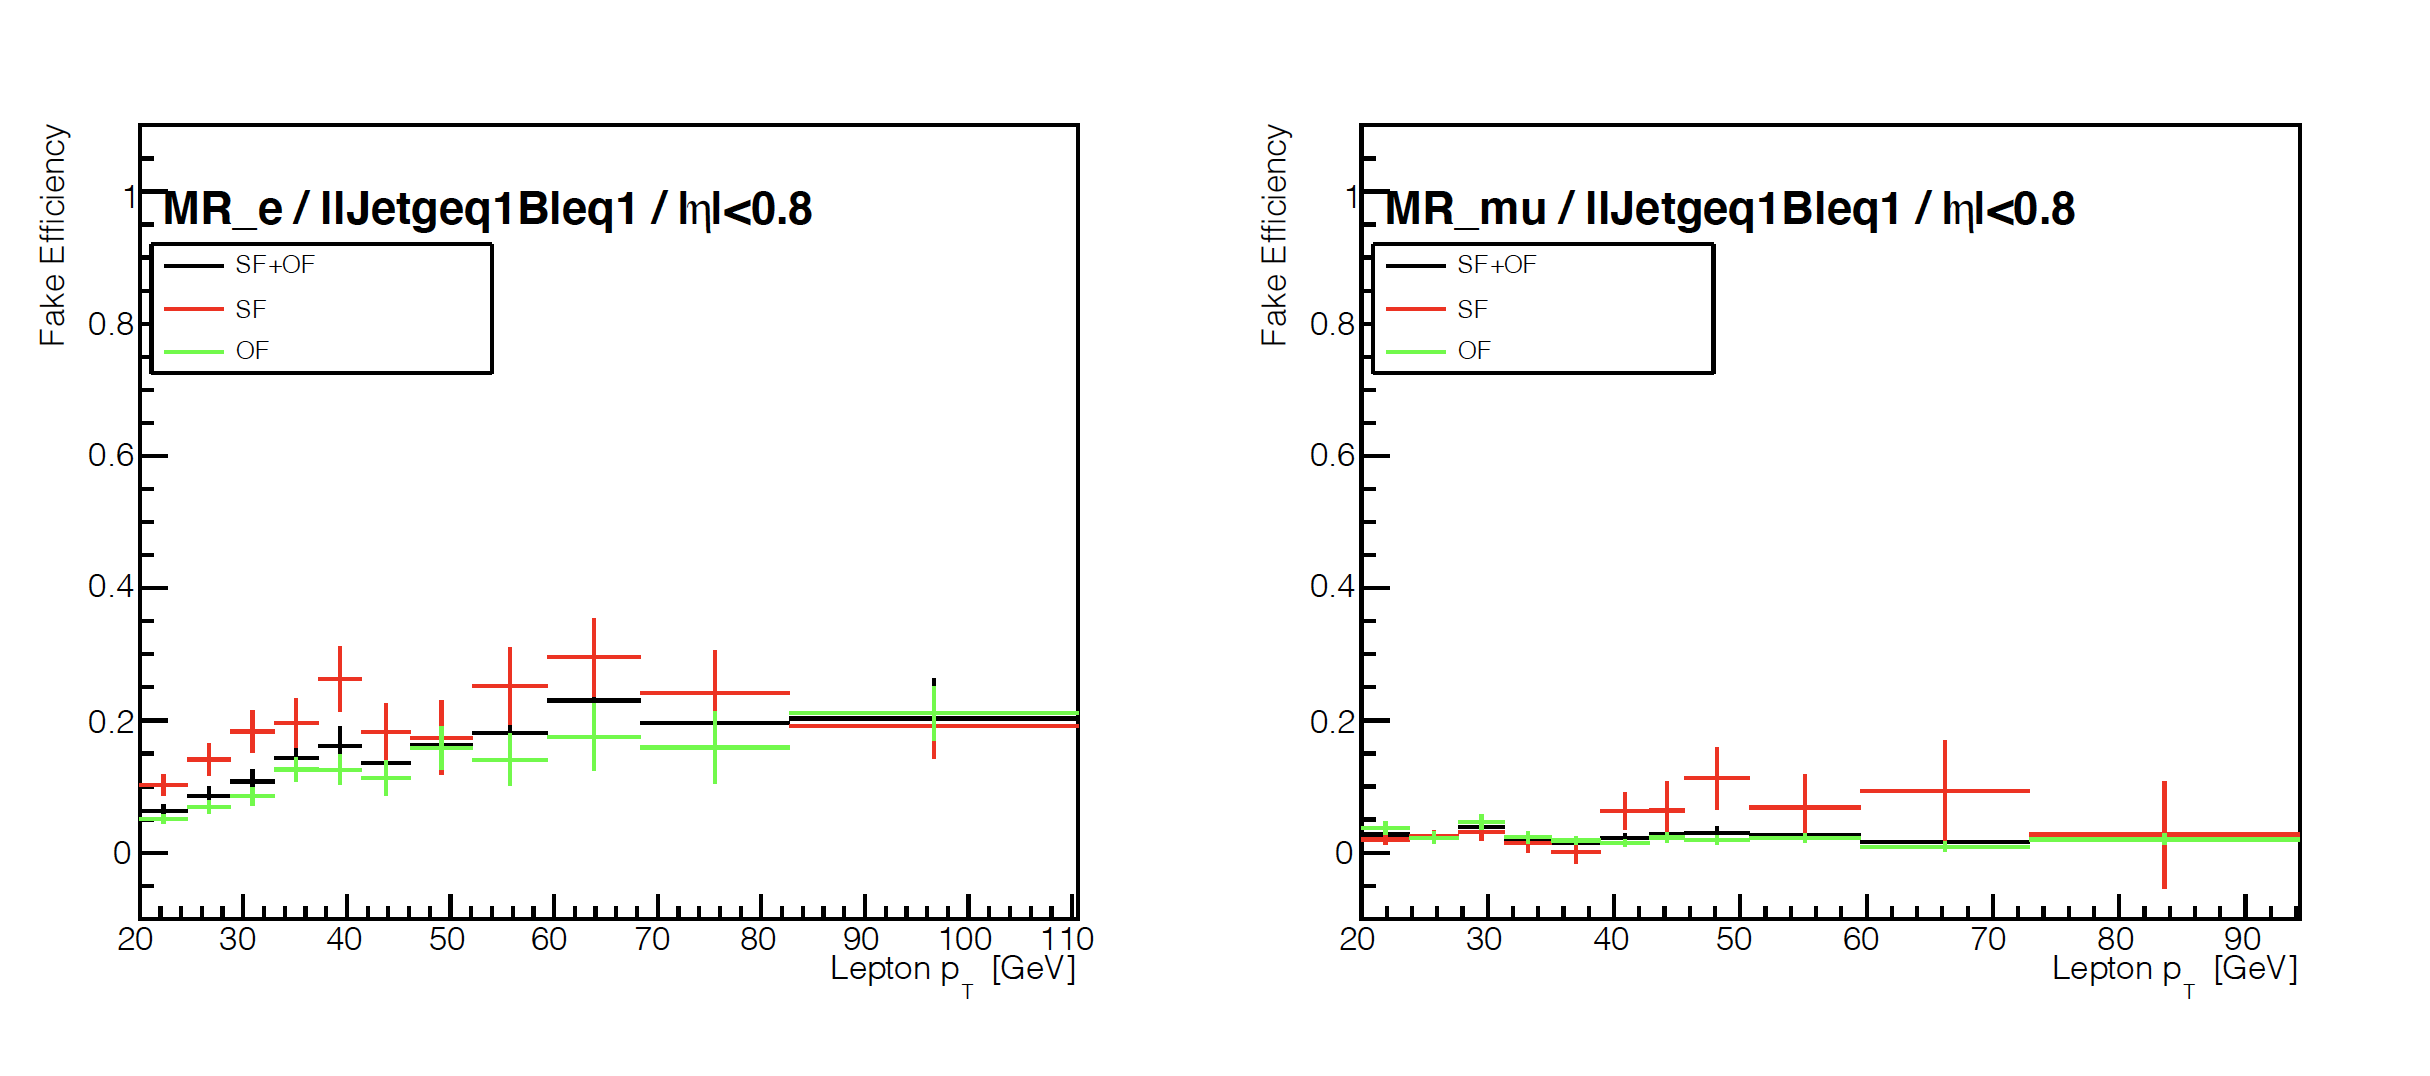
\includegraphics[width=0.85\textwidth]{figures/Part3/Nonprompt/MR/fake_eff}
 \end{tabular}
 \caption{Representative \emph{nonprompt} electron efficiency measured in data events. From left to right: electron $f$, muon $f$. Events with a same-flavor lepton pair are shown in red points while events selected with a different-flavor lepton pair are shown in green points. Events with a same-flavor or different-flavor lepton pair is shown in black points. These plots correspond to the first $|\eta|$ bin ($|\eta|<$0.8) and the second jet multiplicity bin. Events selected Error bars displayed in these plots include statistical uncertainty only. }
 \label{fig:fake_eff}
 \end{center}
\end{figure}

The measured \emph{nonprompt} efficiency $f$ exhibits a dependency on flavor composition, as is shown in Figure~\ref{fig:fake_eff}. This dependency is treated as a source of the systematic uncertainties of the \emph{nonprompt} estimation and is further discussed in \autoref{sec:NonUnc}.

The \emph{prompt} efficiency $r$ is measured in simulated $\ttbar$ events in opposite-sign dilepton regions. The same lepton selection listed in Table~\ref{tab:looseandtight} is used to perform the \emph{Tag-and-Probe}. The leading lepton in $\pt$ is used as a \emph{tag} while the oppositely charged sub-leading lepton is taken as a \emph{probe}. The variation of $r$ between different flavor composition is negligible, as is shown in Figure~\ref{fig:real_eff}. Therefore, only e$\upmu$ events are used to measure \emph{prompt} efficiency in order to minimise the contamination of \emph{nonprompt} leptons.

\begin{figure}[tbh!]
 \begin{center}
 \begin{tabular}{c}
 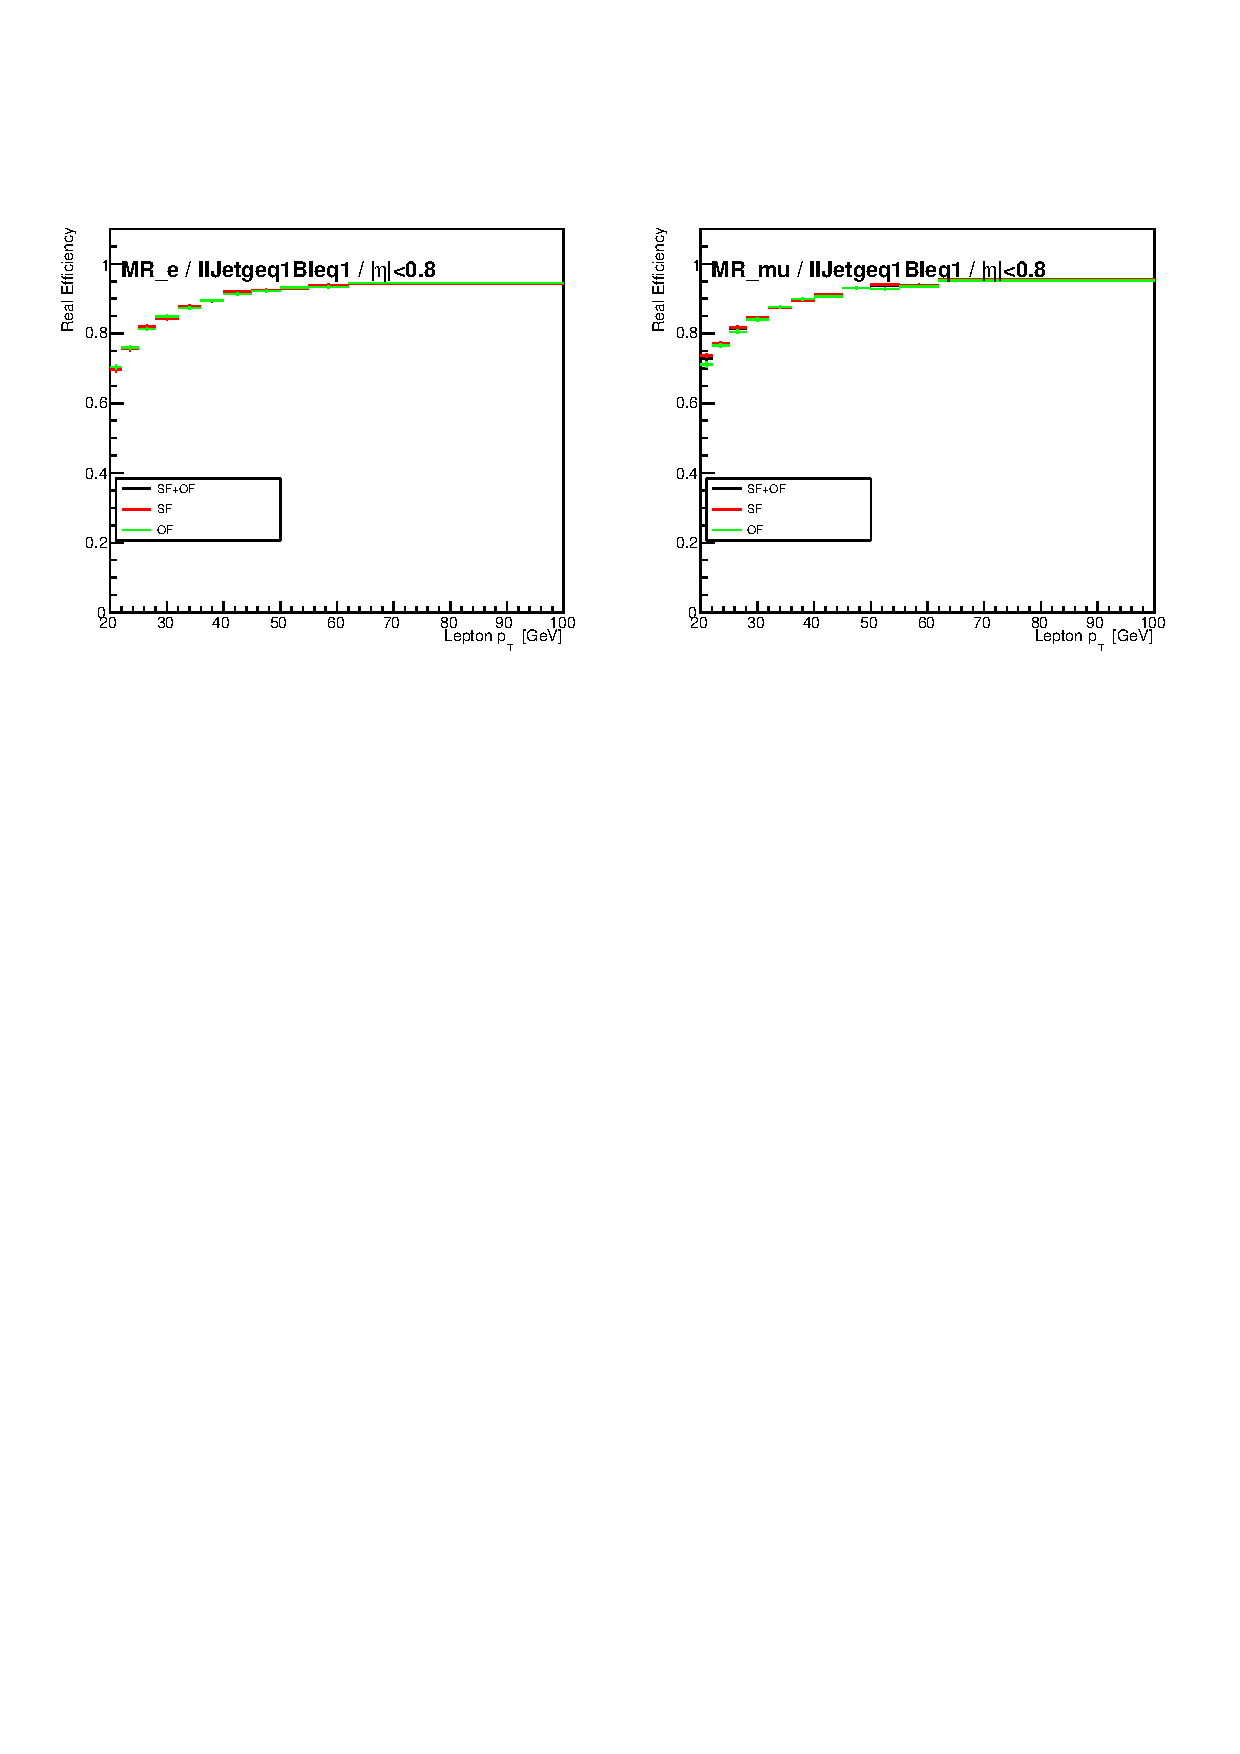
\includegraphics[width=0.85\textwidth]{figures/Part3/Nonprompt/MR/real_eff}
 \end{tabular}
 \caption{Representative \emph{prompt} efficiency measured in simulated $\ttbar$ events. From left to right: electron $r$, muon $r$. Events with a same-flavor lepton pair are shown in red points while events selected with a different-flavor lepton pair are shown in green points. Events with a same-flavor or different-flavor lepton pair is shown in black points. These plots correspond to the first $|\eta|$ bin ($|\eta|<$0.8) and the second jet multiplicity bin. Error bars displayed in these plots include statistical uncertainty only. }
 \label{fig:real_eff}
 \end{center}
\end{figure}

The selection criteria for various \acp{MR} is summarised in Table~\ref{tab:MR}.

\begin{table}[th]
\sffamily
\centering
\resizebox{\textwidth}{!}{ 
\begin{tabular}{cccccccc}
\toprule
\multirow{2}{*}{Observable}   & \multirow{2}{*}{jet bin}          &  \multirow{2}{*}{\vtop{\hbox{\strut $\#$ of selected}\hbox{\strut~~~leptons}}} &   \multirow{2}{*}{\vtop{\hbox{\strut lepton flavor}\hbox{\strut~composite}}} & \multirow{2}{*}{$|\sum_iC_i|$} & \multirow{2}{*}{OffZ}               &  \multirow{2}{*}{njet}  & \multirow{2}{*}{nbjet}\\ 
   &  &  &   &  &                &    & \\ \midrule
\multirow{2}{*}{$f$}     & 0 jet                & 2                                & any                                   & 2                       & same-sign ee   & = 0                    & = 0   \\  
                                   & 1 or more jet  & 2                                &  any                                  & 2                         &  same-sign ee    & $\geq$ 1 & $\leq$ 1\\ \midrule
\multirow{2}{*}{$r$}    & 0 jet                & 2                                 & e$\upmu$ only                     & 0                        & -    & = 0                      & = 0     \\  
                                 & 1 or more jet  & 2                                  & e$\upmu$ only                      & 0                        & -      & $\geq$ 1 & $\leq$ 1 \\ \bottomrule  
\end{tabular}
}
\caption{Summary of the cuts applied to the $r$/$f$ measurement region.}
\label{tab:MR}
\end{table}
%%%%%%%%%%%%%%%%%%%%%%%%%%%%%%%%%%%%%%%%%%%%%%%%%%%%%%%%%%%%
%%%%%%%%%%%%%%%%%%%%%%%%%%%%%%%%%%%%%%%%%%%%%%%%%%%%%%%%%%%%

\section{Validation of the Matrix Method}
\label{sec:MMVR}

The performance of the \mm~is validated using three regions that are tangential to the \ac{SR}, referred to as \acp{VR}. In these \acp{VR}, \emph{prompt} backgrounds are estimated using \ac{MC} simulation while \emph{nonprompt} background is estimated with the \mm. A summary of the selections applied to these VRs is given in \autoref{chap:Selection}. 

Distribution of the leading lepton $\eta$ and jet multiplicity are shown in Figure~\ref{fig:VR_matrix}. Good agreement between data and background estimate has been observed in all three \acp{VR}.

\begin{figure}[tbh!]
 \begin{center}
 \begin{tabular}{cc}
 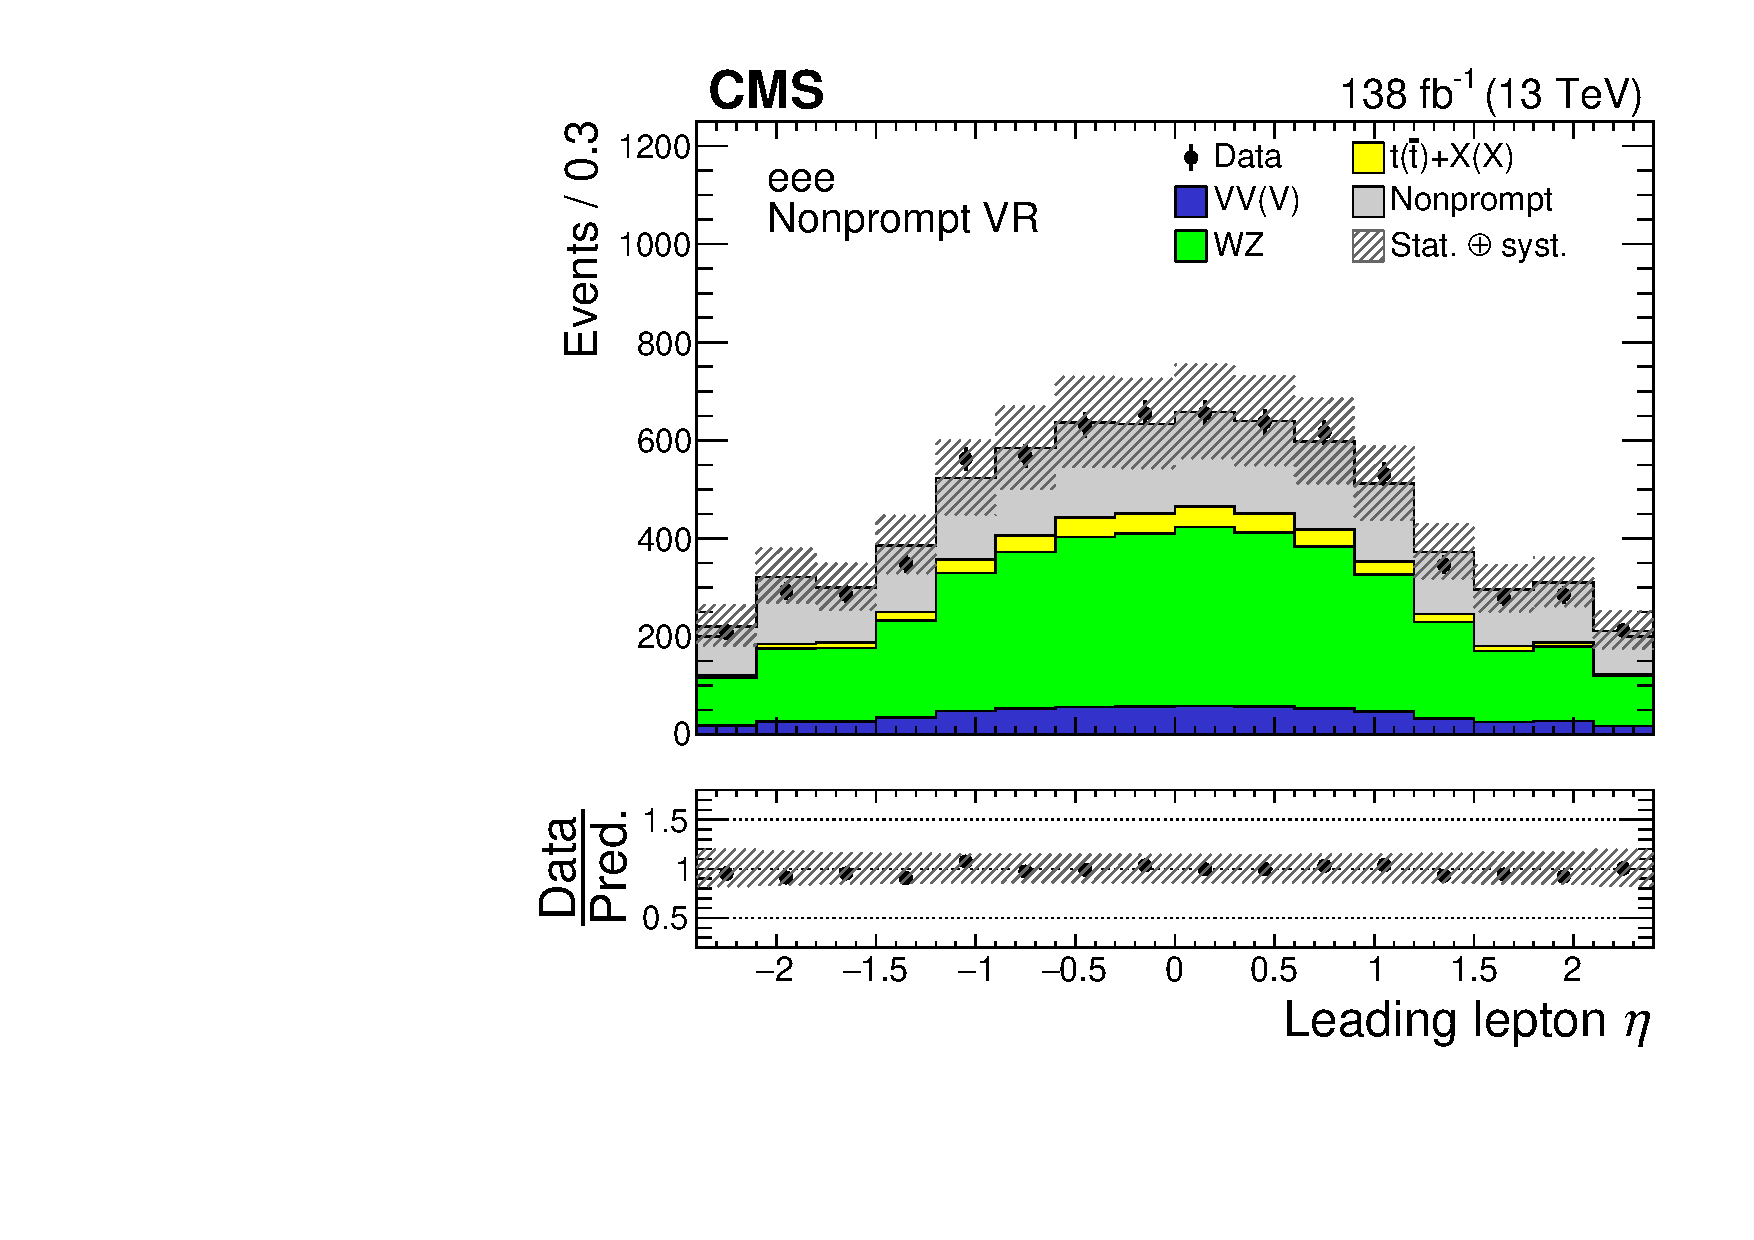
\includegraphics[width=0.45\textwidth]{figures/Part3/Nonprompt/VR/eee/lep1Eta}&
 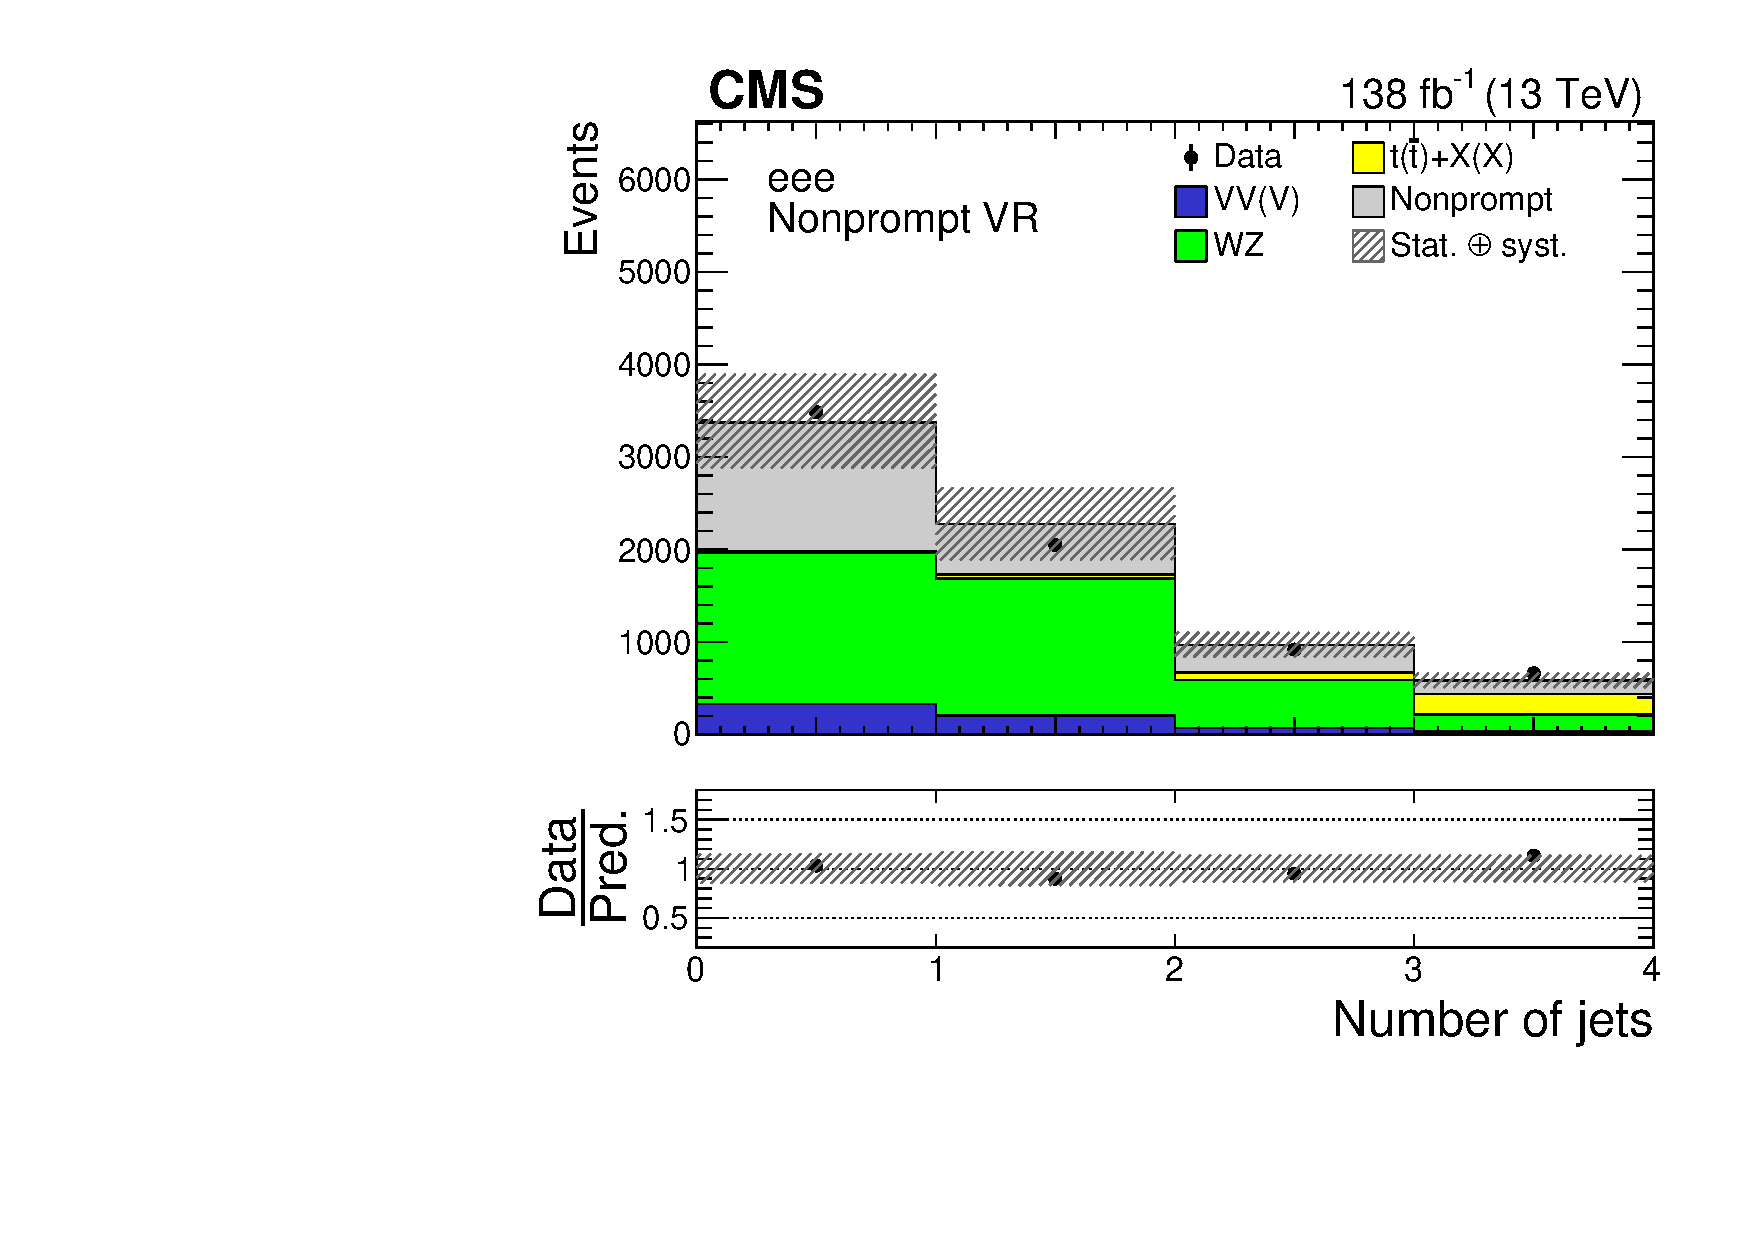
\includegraphics[width=0.45\textwidth]{figures/Part3/Nonprompt/VR/eee/njet} \\
   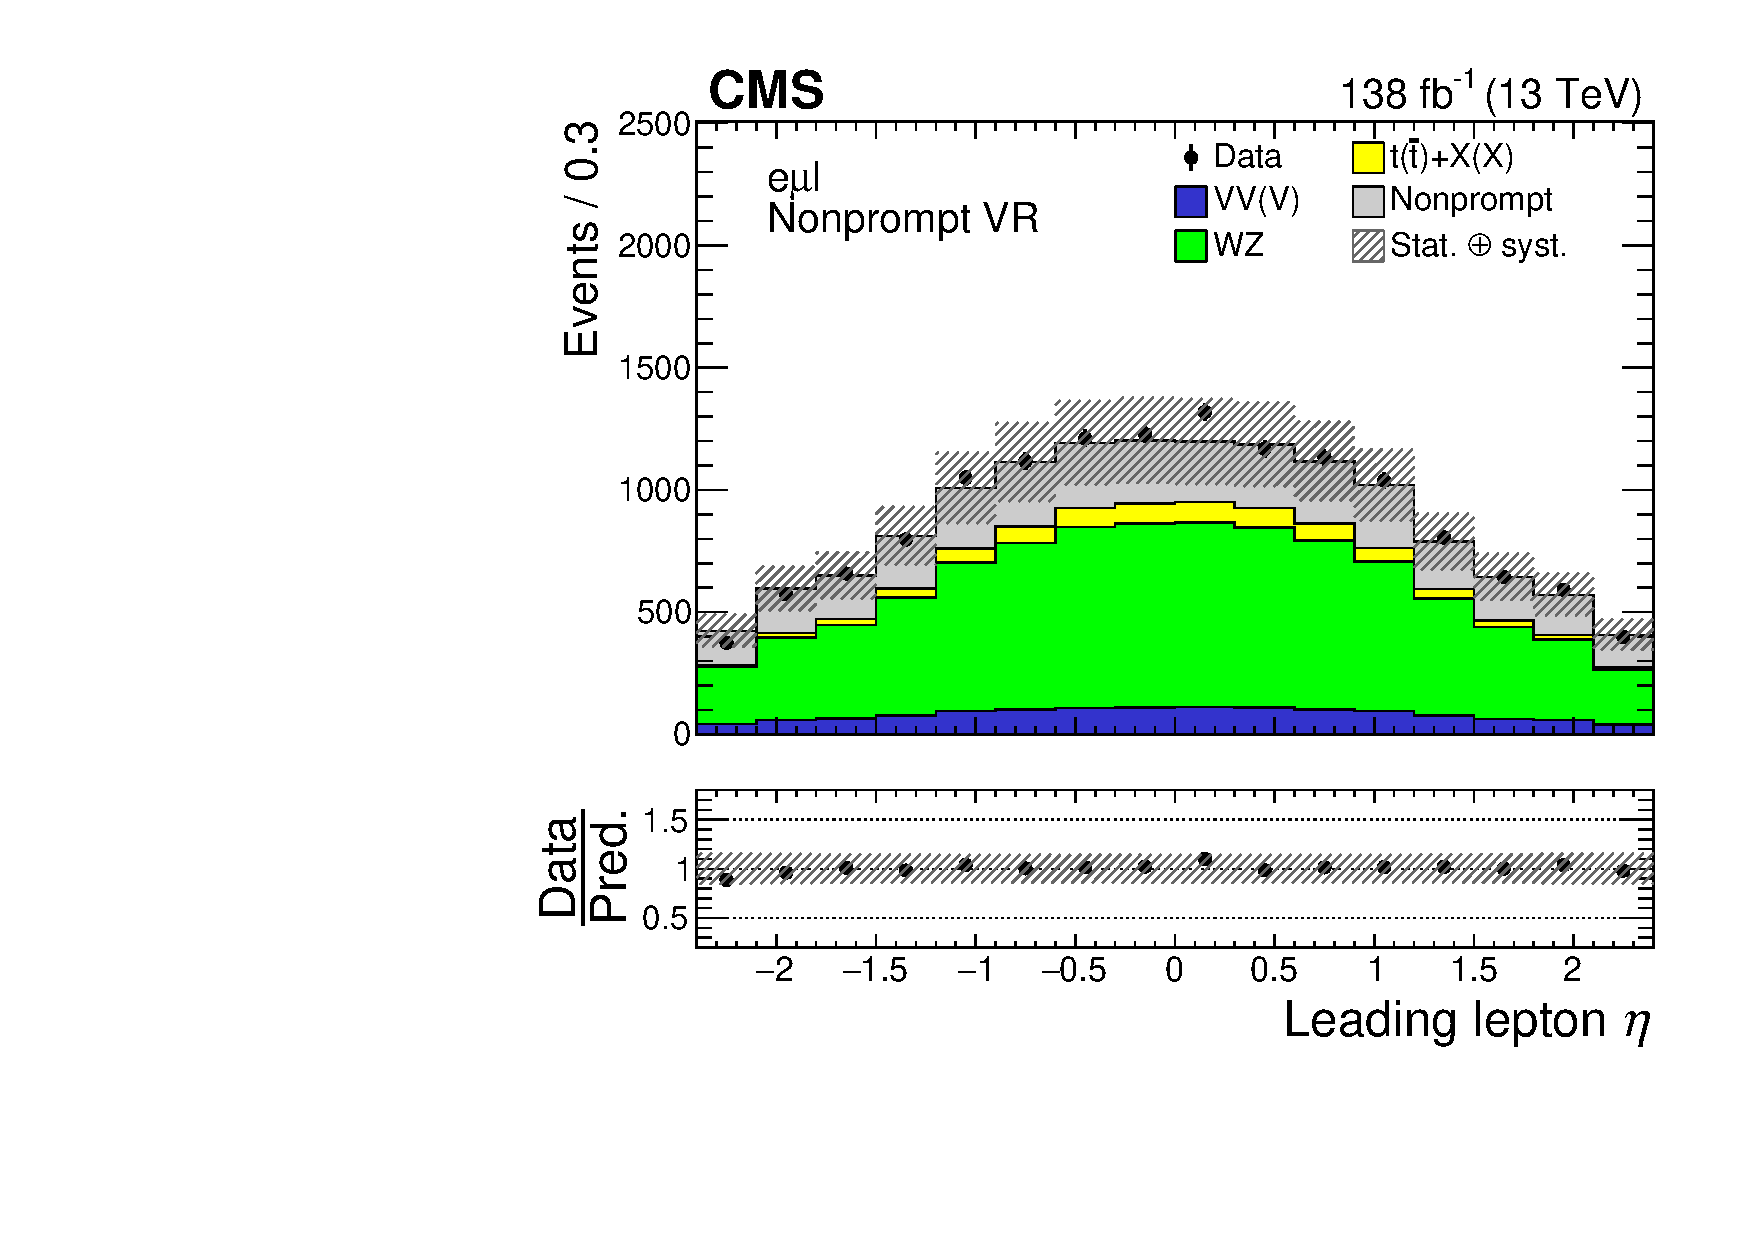
\includegraphics[width=0.45\textwidth]{figures/Part3/Nonprompt/VR/emul/lep1Eta}&
 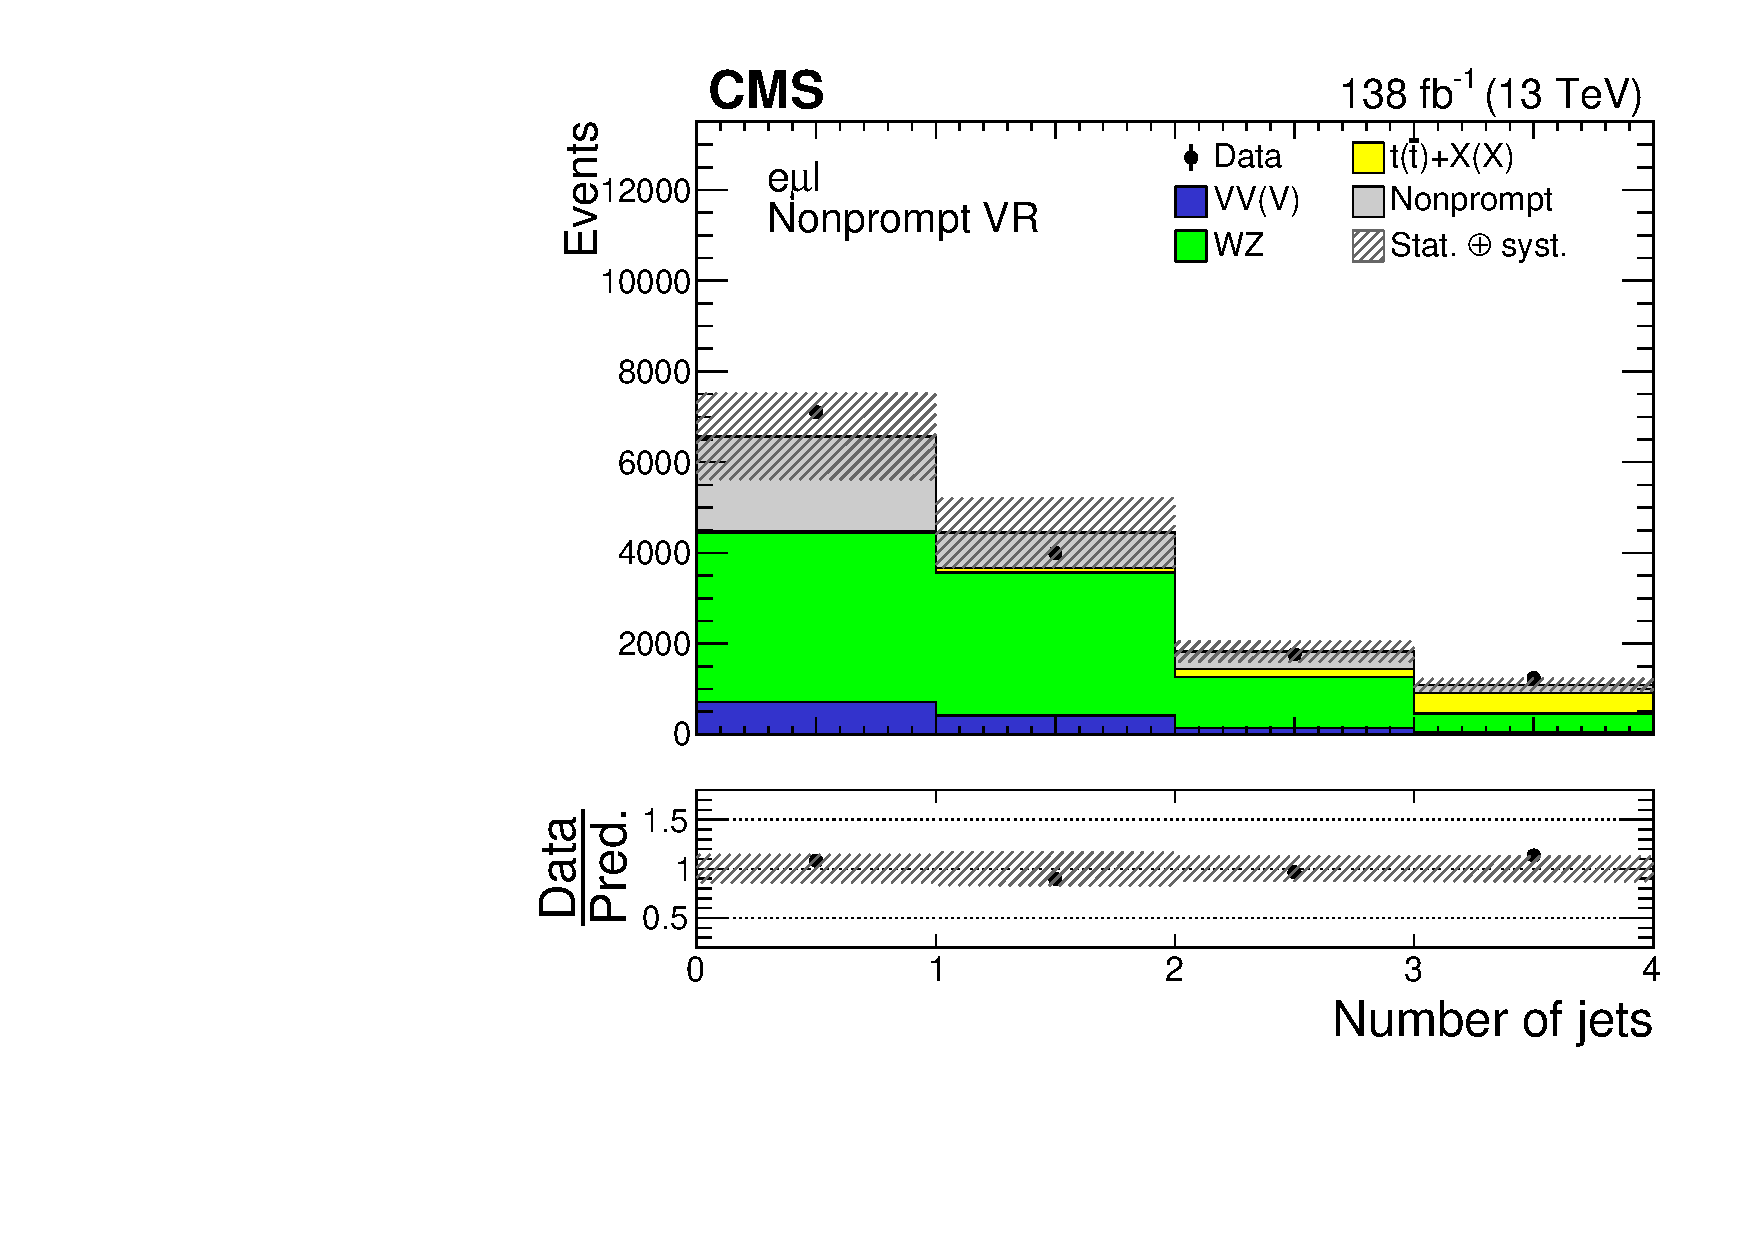
\includegraphics[width=0.45\textwidth]{figures/Part3/Nonprompt/VR/emul/njet} \\
    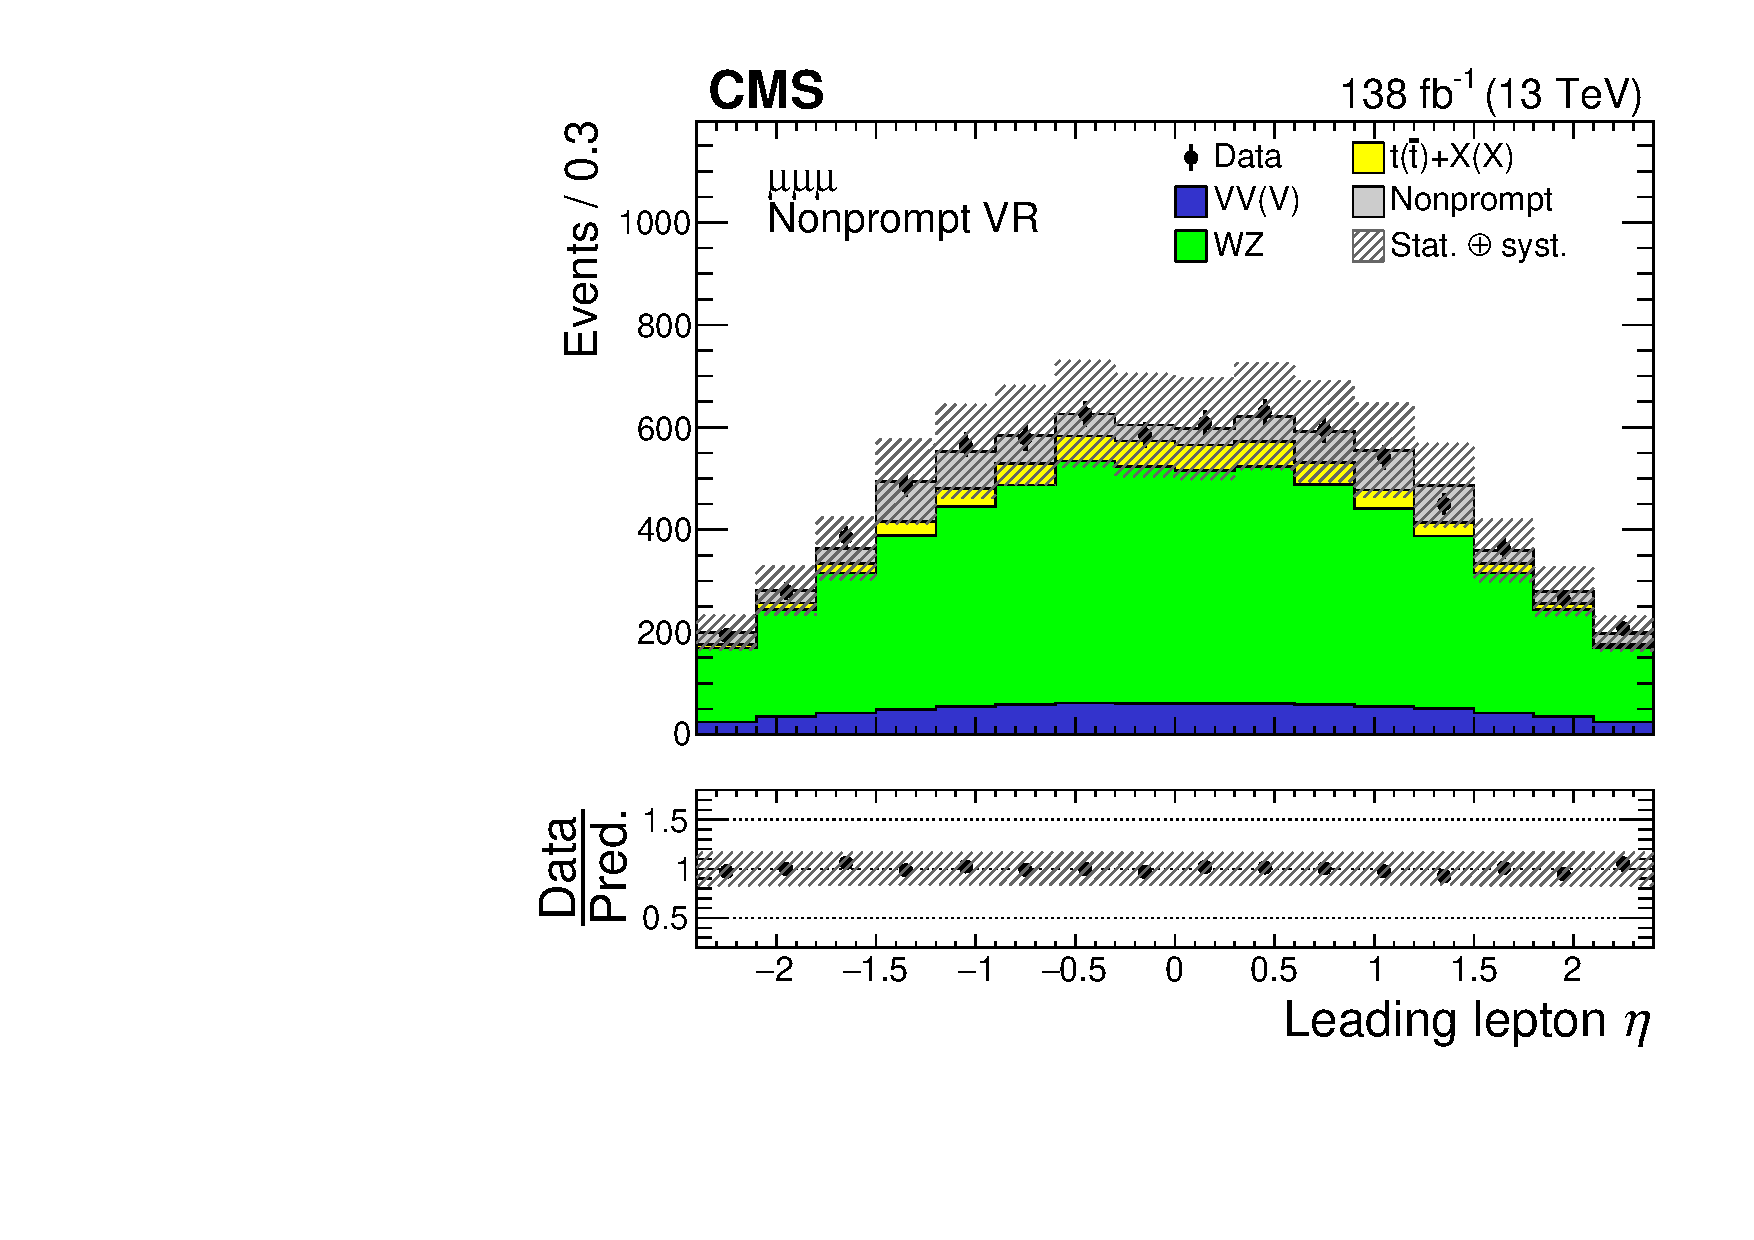
\includegraphics[width=0.45\textwidth]{figures/Part3/Nonprompt/VR/mumumu/lep1Eta}&
 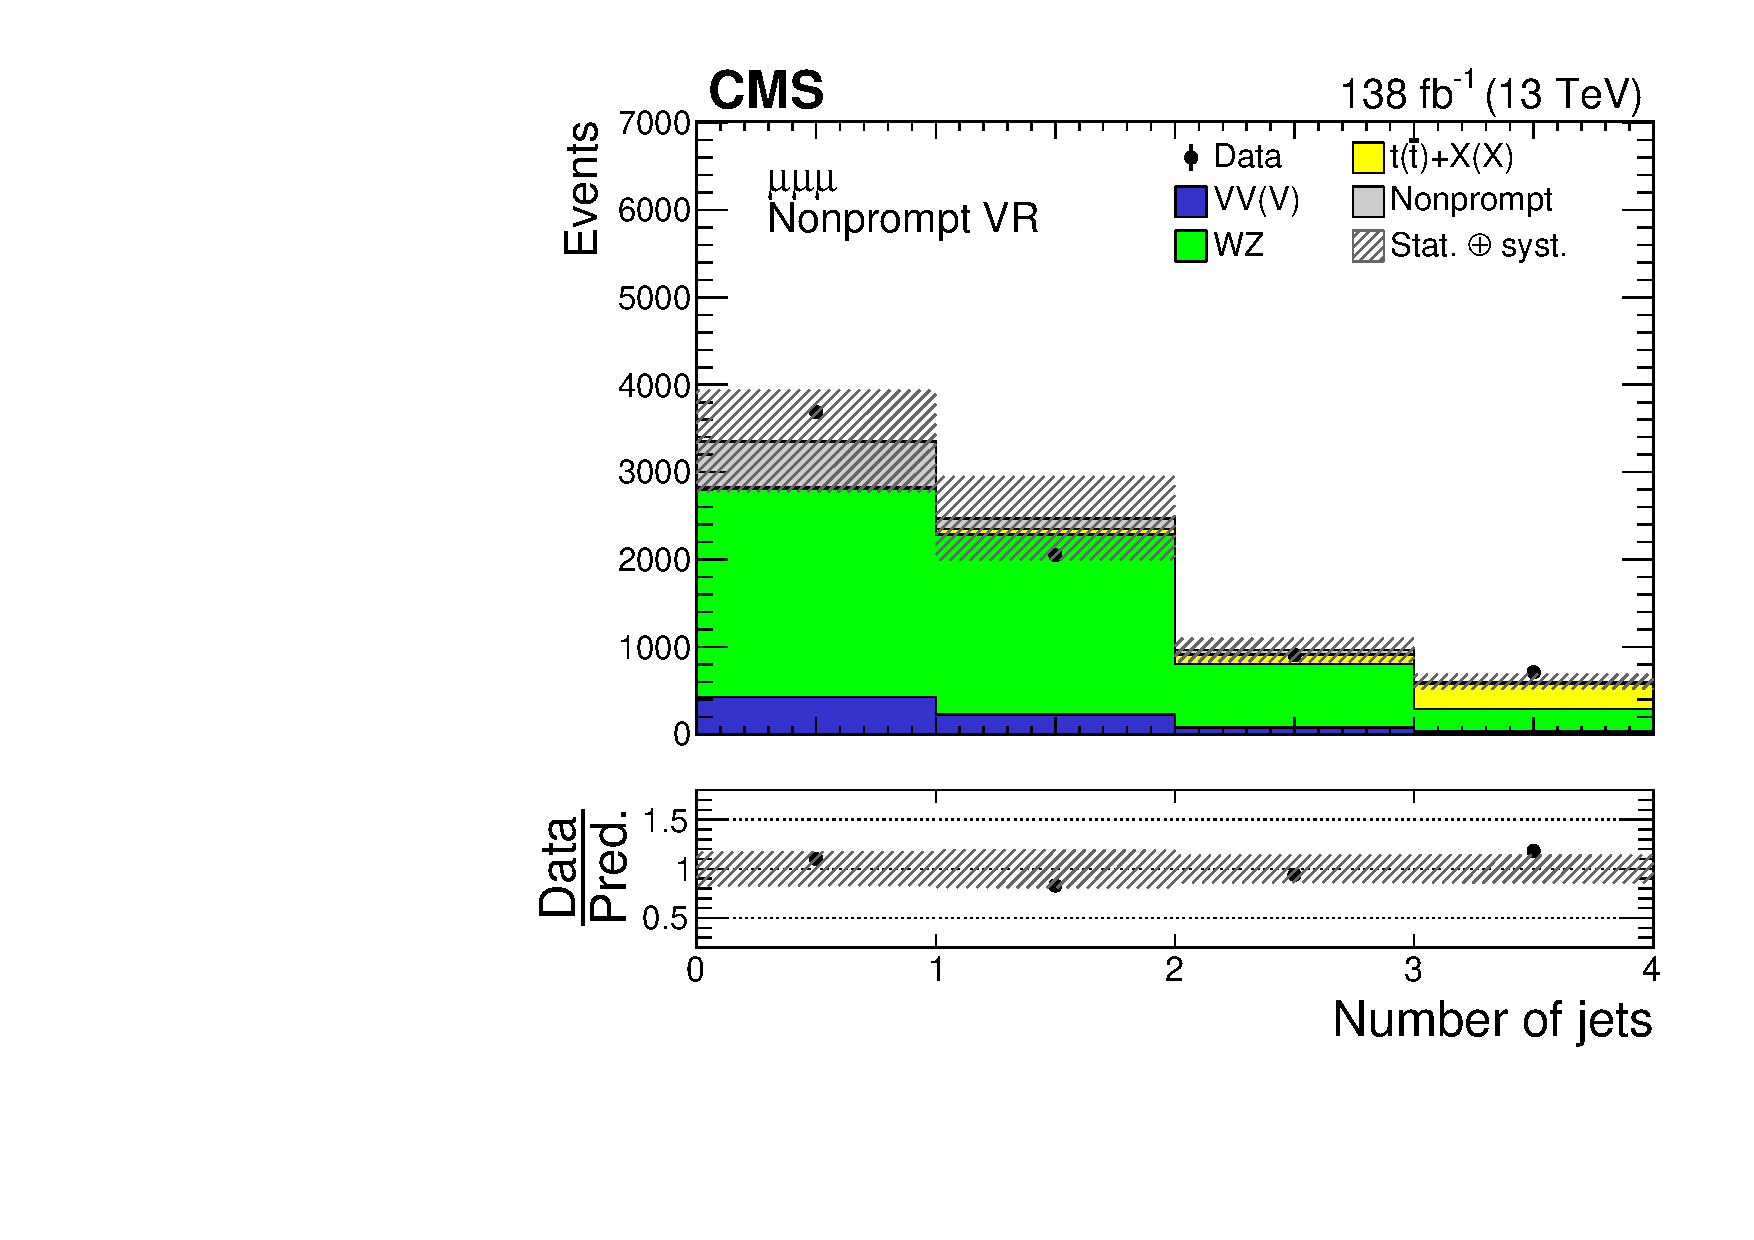
\includegraphics[width=0.45\textwidth]{figures/Part3/Nonprompt/VR/mumumu/njet} \\
 \end{tabular}
 \caption{Distributions of the leading lepton $\eta$ (left column) and the jet multiplicity (right column) in the \emph{nonprompt} \acp{VR}. Events in the eee, $\emul$, and $\mmm$ \emph{nonprompt} \acp{VR} are shown in the upper, middle, and lower row, respectively. The data are shown as filled points and the \ac{SM} background predictions as histograms. The \emph{nonprompt} background is estimated using control samples in data, while other backgrounds are estimated using \ac{MC} simulation. The hatched bands indicate statistical and systematic uncertainties for the \ac{SM} background predictions. The last bin of the right histogram includes the overflow events.}
 \label{fig:VR_matrix}
 \end{center}
\end{figure}
%%%%%%%%%%%%%%%%%%%%%%%%%%%%%%%%%%%%%%%%%%%%%%%%%%%%%%%%%%
%%%%%%%%%%%%%%%%%%%%%%%%%%%%%%%%%%%%%%%%%%%%%%%%%%%%%%%%%%

\section{Nonprompt Estimate in SR}
\label{sec:MMSR}

The \mm~is used to estimate \emph{nonprompt} background in the \ac{SR}. Distributions of the LFV e$\upmu$ mass and the Z boson mass are shown in Figure~\ref{fig:SR_DataDriven_1}. When compared to background estimate from pure \ac{MC} simulation (Figure~\ref{fig:SR}), the updated background template is smoother with lower statistical uncertainties. 

\begin{figure}[tbh!]
 \begin{center}
 \begin{tabular}{cc}
  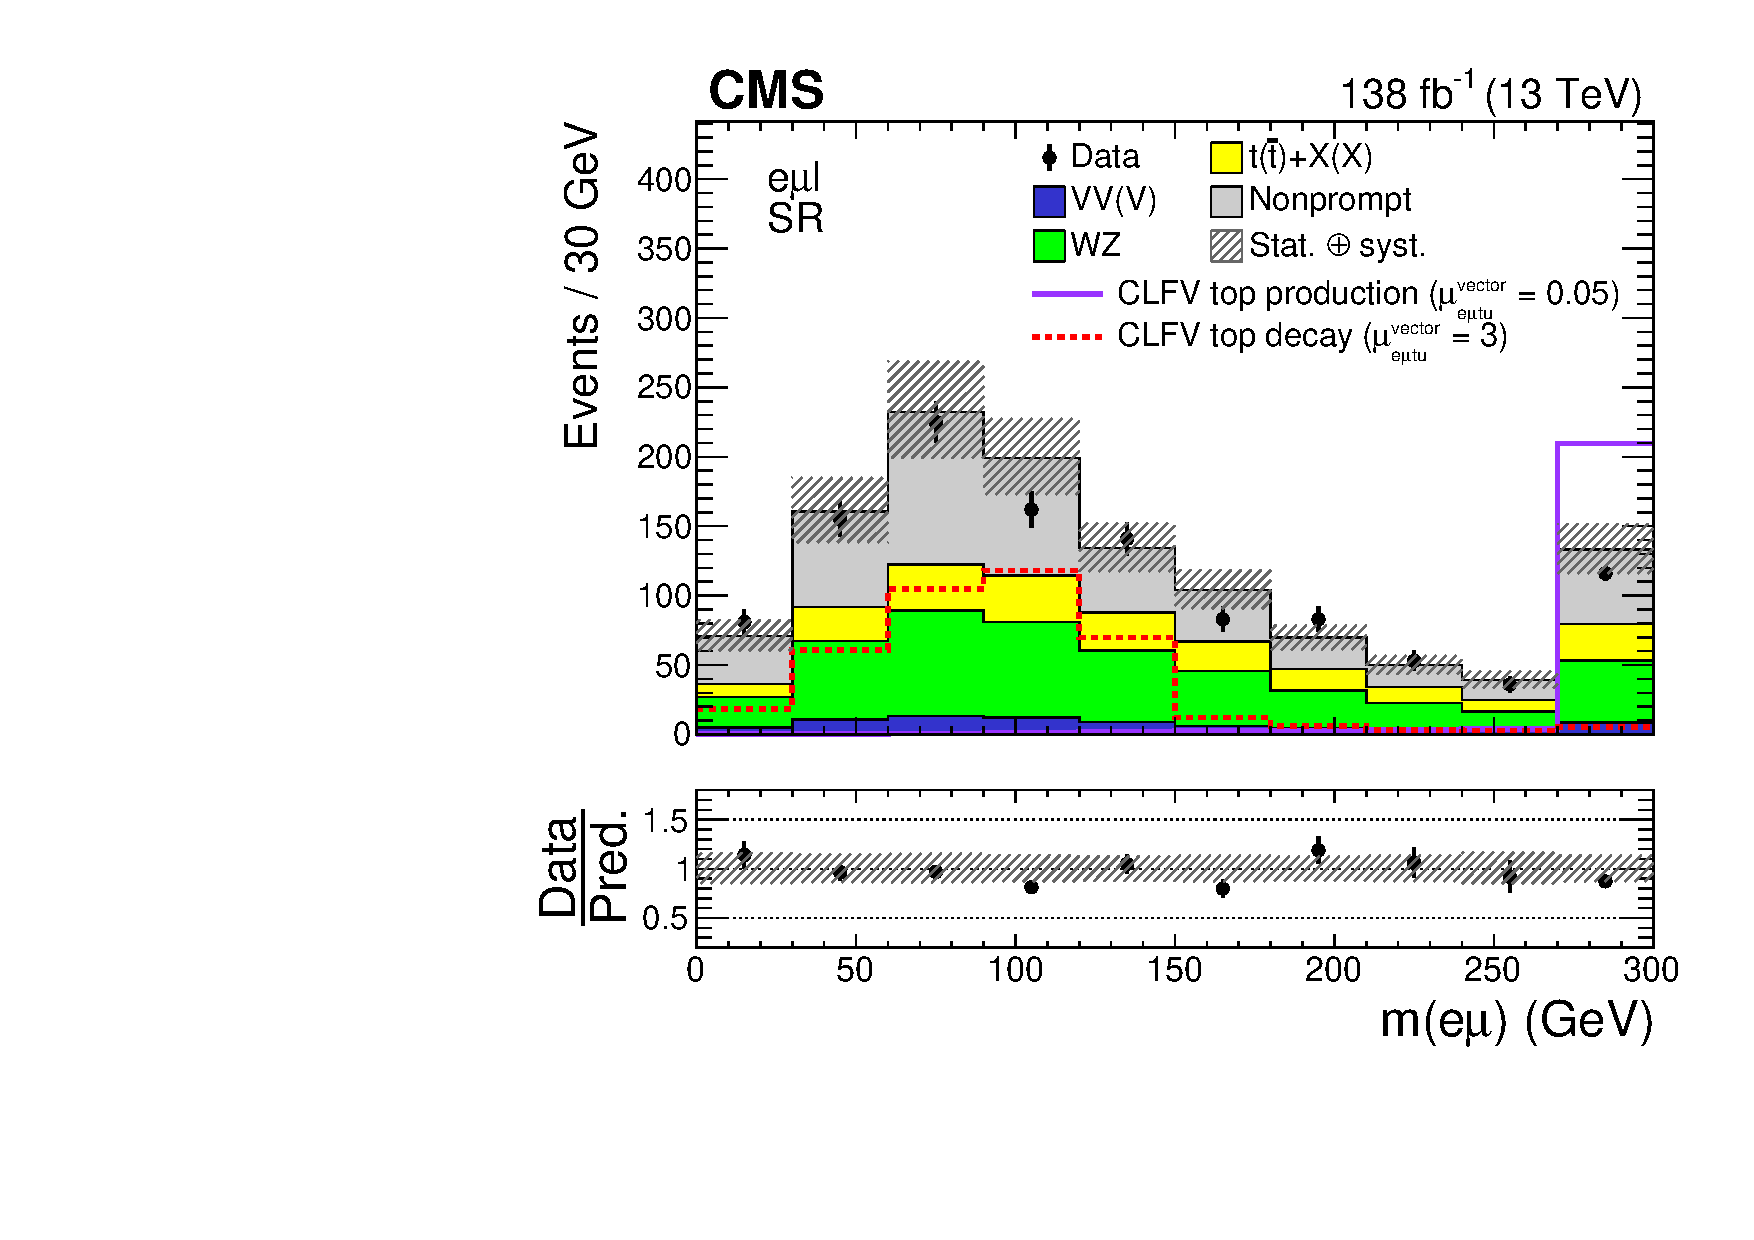
\includegraphics[width=0.45\textwidth]{figures/Part3/Nonprompt/SR/Memu}&
 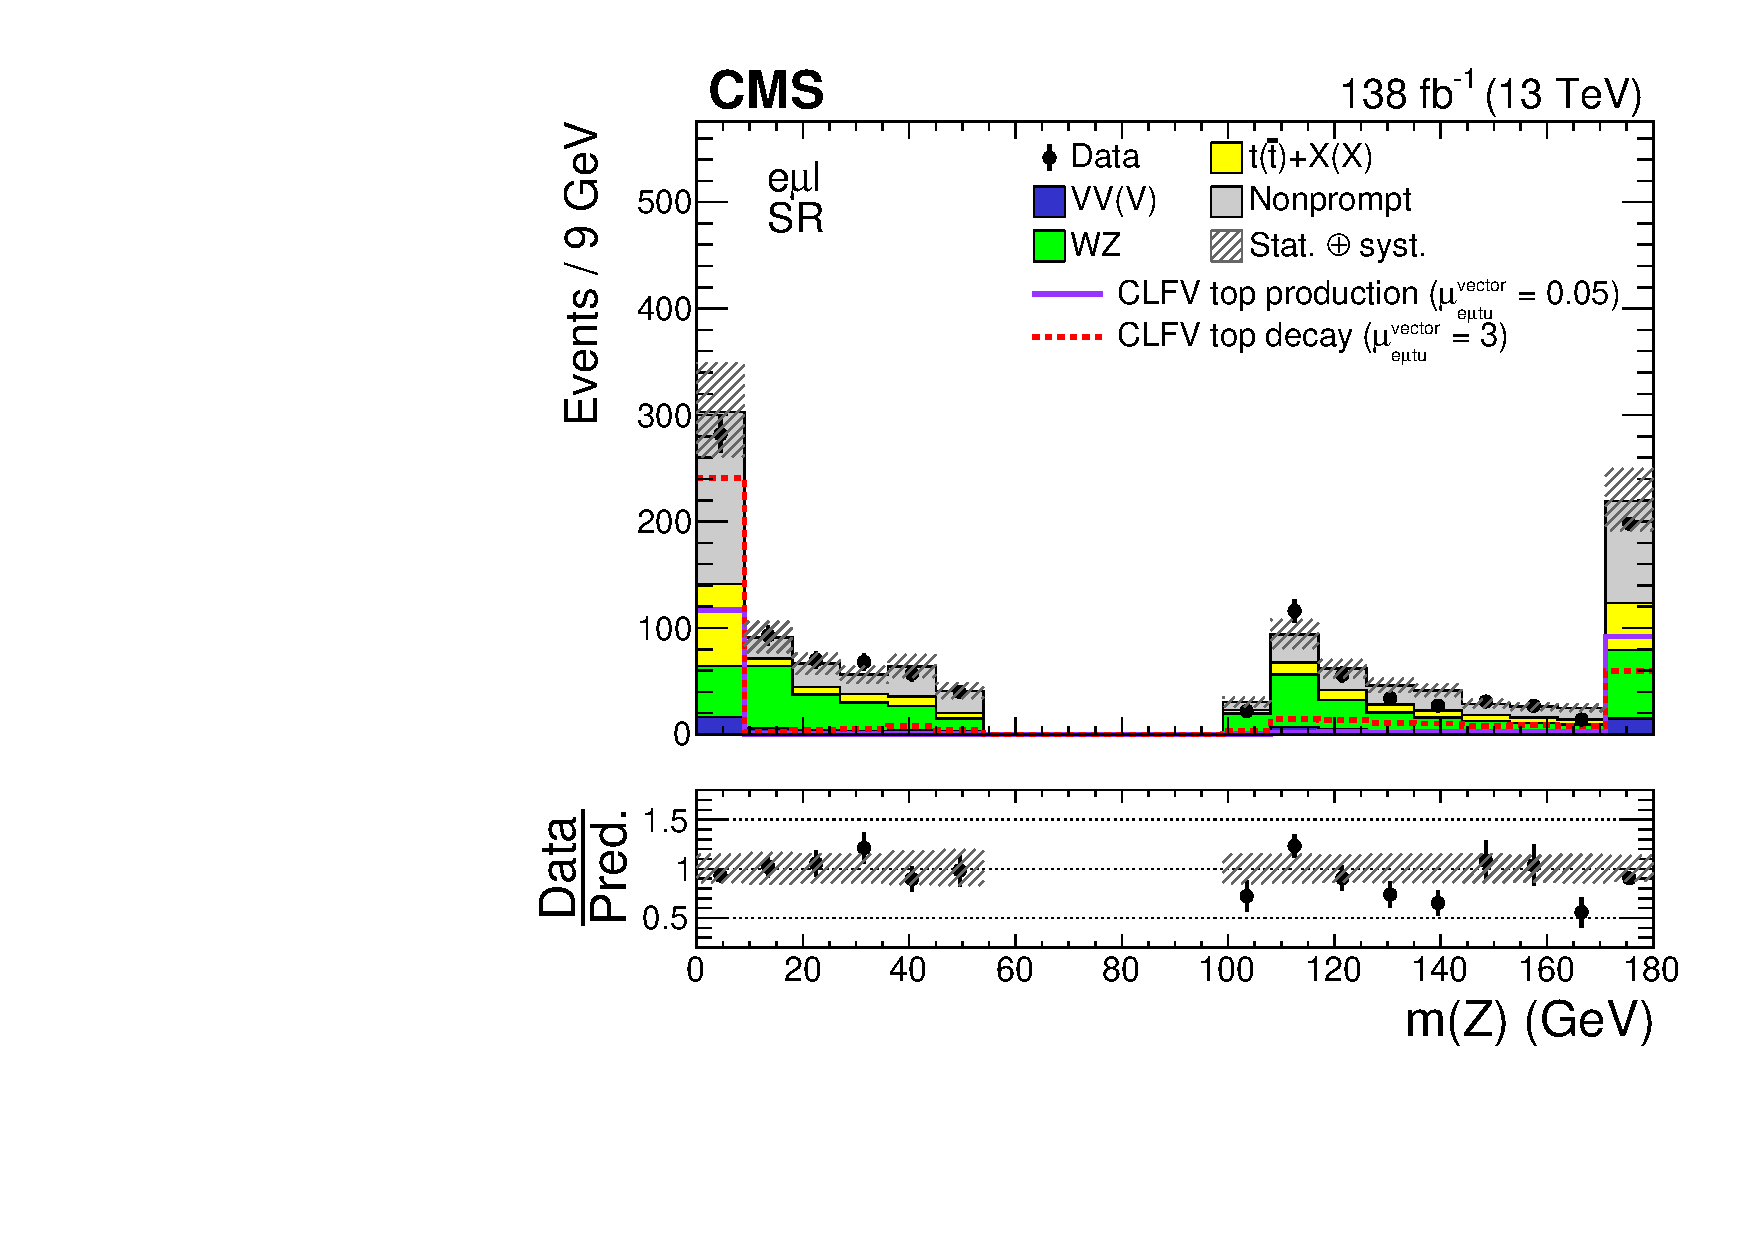
\includegraphics[width=0.45\textwidth]{figures/Part3/Nonprompt/SR/Zmass} \\
 \end{tabular}
 \caption{Distributions of the LFV e$\upmu$ mass (left) and the Z boson mass (right) in \ac{SR}. The data are shown as filled points and the \ac{SM} background predictions as histograms. The \emph{nonprompt} background is estimated using control samples in data, while other backgrounds are estimated using \ac{MC} simulation. The hatched bands indicate statistical and systematic uncertainties for the \ac{SM} background predictions. The normalisation of the signal processes is chosen arbitrarily for improved visualisation. The last bin of both histograms includes the overflow events.}
 \label{fig:SR_DataDriven_1}
 \end{center}
\end{figure}

The number of expected events from various kinds of backgrounds are shown in Table \ref{tab:eventcount}. 

\begin{table}[th]
\sffamily
\centering
\caption{Expected background contributions and the number of events observed in data collected during 2016--2018. The statistical and systematic uncertainties are added in quadrature. The category ``other backgrounds'' includes smaller background contributions containing one or two top quarks plus a boson or quark. The \ac{CLFV} signal, generated with $\WC{\textsf{vector}}{\emut{u}}/\Lam^2=1\TeV^{-2}$, is also listed for reference. The signal yields include contributions from both top production and decay modes.}
\begin{tabular}{ccc}
\toprule
Process & m(e$\upmu$)<150 GeV & m(e$\upmu$)>150 GeV \\
\midrule
Nonprompt & $351\pm92$ & $146\pm38$\\
WZ & $275\pm64$ & $145\pm35$\\
ZZ & $33.2\pm6.5$ & $13.1\pm2.6$\\
VVV & $17.0\pm8.5$ & $12.0\pm6.0$\\
$\ttbar$W & $47.6\pm10.0$ & $40.0\pm9.1$\\
$\ttbar$Z & $39.1\pm7.9$ & $25.8\pm5.4$\\
$\ttbar$H & $28.2\pm4.5$ & $10.0\pm1.6$\\
tZq & $5.5\pm1.1$ & $2.5\pm0.5$\\
Other & $7.3\pm3.7$ & $4.5\pm2.3$\\
Total expected & $805\pm123$ & $398\pm57$\\
Data & 783 & 378\\
\midrule
CLFV & $207\pm15$ & $4440\pm215$\\
\bottomrule
\end{tabular}
\label{tab:eventcount}
\end{table}

\chapter{Signal Extraction with Boosted Decision Trees}
\label{chap:BDT}

A \ac{MVA} is performed in \ac{SR} to further separate the LFV signals from the backgrounds, and enhance the sensitivity of this analysis. More specifically, a dozen of discriminating variables, referred to as ``features'', are selected and combined by a gradient-\ac{BDT}, which is implemented using the \textsc{XGBoost} package \cite{Chen:2016:XST:2939672.2939785}. There are several reasons why \ac{BDT} is chosen: (i) the goal of the \ac{MVA} is to achieve maximum separation between signals and backgrounds using a small number of already well-separated kinematic variables, instead of exploring some complicated structures hidden in event topology, (ii) under such a goal, the potential performance gain from a more sophisticated algorithm like a \ac{NN} is limited, (iii) a \ac{BDT}-based algorithm is straightforward to implement and consumes only a moderate amount of computational resources, and (iv) the interpretability of a \ac{BDT}-based algorithm is excellent. 

The top production and decay signals are longer distinguished by the \ac{BDT}. They are combined into a single signal class, just like all backgrounds are combined into a single background class. The training of the \ac{BDT} depends entirely on \ac{MC} samples that are statistically orthogonal to the samples used in the actual background estimation. More details on the configurations of the \ac{BDT} are described in \autoref{sec:Config}. The input features are described in \autoref{sec:Input}. The output of the \ac{BDT} is presented in \autoref{sec:Output}.
%%%%%%%%%%%%%%%%%%%%%%%%%%%%%%%%%%%%%%%%%%%%%%%%%%%%%%%%%%
%%%%%%%%%%%%%%%%%%%%%%%%%%%%%%%%%%%%%%%%%%%%%%%%%%%%%%%%%%

\section{BDT Configuration}
\label{sec:Config}

The LFV e$\upmu$ mass of the top decay signal is bounded by the \ac{SM} top quark mass, as is shown in Figure~\ref{sec:SR}. On the contrary, the LFV e$\upmu$ mass of the top production signal has no such restriction and often reaches TeV level. Therefore, a 150 GeV threshold is used to divide the \ac{SR} into two \acp{SR} enriched in different signal modes. The \ac{MVA} strategy is to combine two signal modes within each \ac{SR} and train binary \acp{BDT} separately for each \ac{SR}. In other words, only two signal datasets and two background datasets are needed.
   
Other aspects of the signal \ac{MC} samples, such as the Lorentz structure and the flavor of the up-type quark involved in LFV interaction, are shown to have a relatively small impact on the kinematics of final state particles, as is shown in Figure~\ref{fig:Lorentz}. Therefore, they are not distinguished by the \ac{BDT}. The selection criteria used to define \ac{SR}, described in \autoref{sec:SR}, are used to preselect events before the construction of both signal and background datasets. 

The construction of the signal datasets take a few steps. Firstly, the cross sections of all top production signal samples, regardless of the Lorentz structure or the quark flavor, are set to the cross section of the vector-like top production signal with an $\emut{u}$ vertex, which is shown in Table~\ref{tab:signal}. This is done to remove poential bias towards the signals with higher cross sections. Similarly, the cross sections of all top decay signal samples are set to the cross section of the vector-like top decay signal. For each sample, a normalisation weight is calculated and is used to replace the original normalisation component of the \ac{MC} weights. These updated \ac{MC} weights are eventually passed on to the \ac{BDT} to weight each signal event.  Secondly, all top production and decay signal samples are combined into a single dataset, which is then sub-divided into two datasets using a 150 GeV threshold on LFV e$\upmu$. The last step is to adjust the overall normalisation (i.e. sum of the \ac{MC} weights) of each of the two signal datasets to match the overall normalisation of the corresponding background dataset. 

\begin{figure}[tbh!]
 \begin{center}
 \begin{tabular}{cc}
  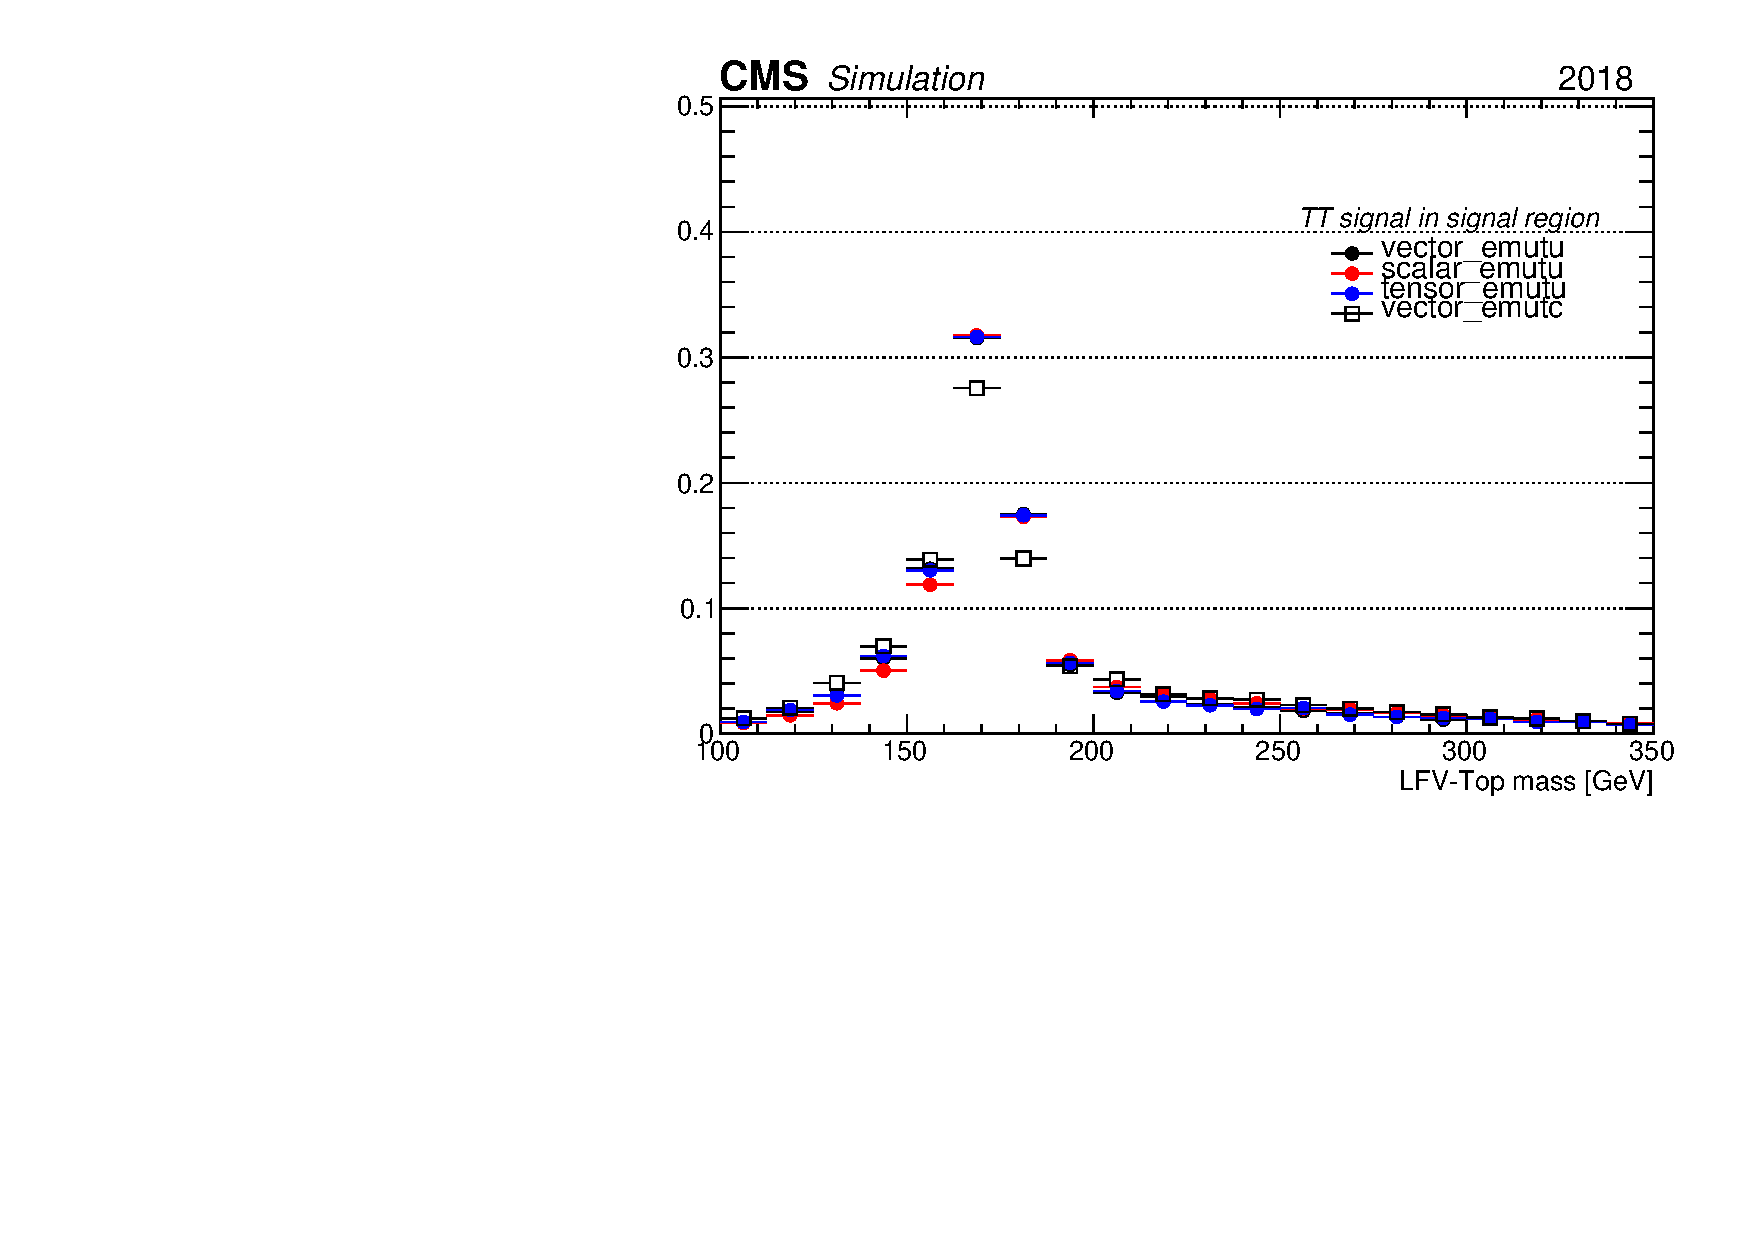
\includegraphics[width=0.48\textwidth]{figures/Part3/BDT/LFV_VR_emul_lllOffZMetg20Jetgeq1Bleq1_LFVTopmass_N}&
    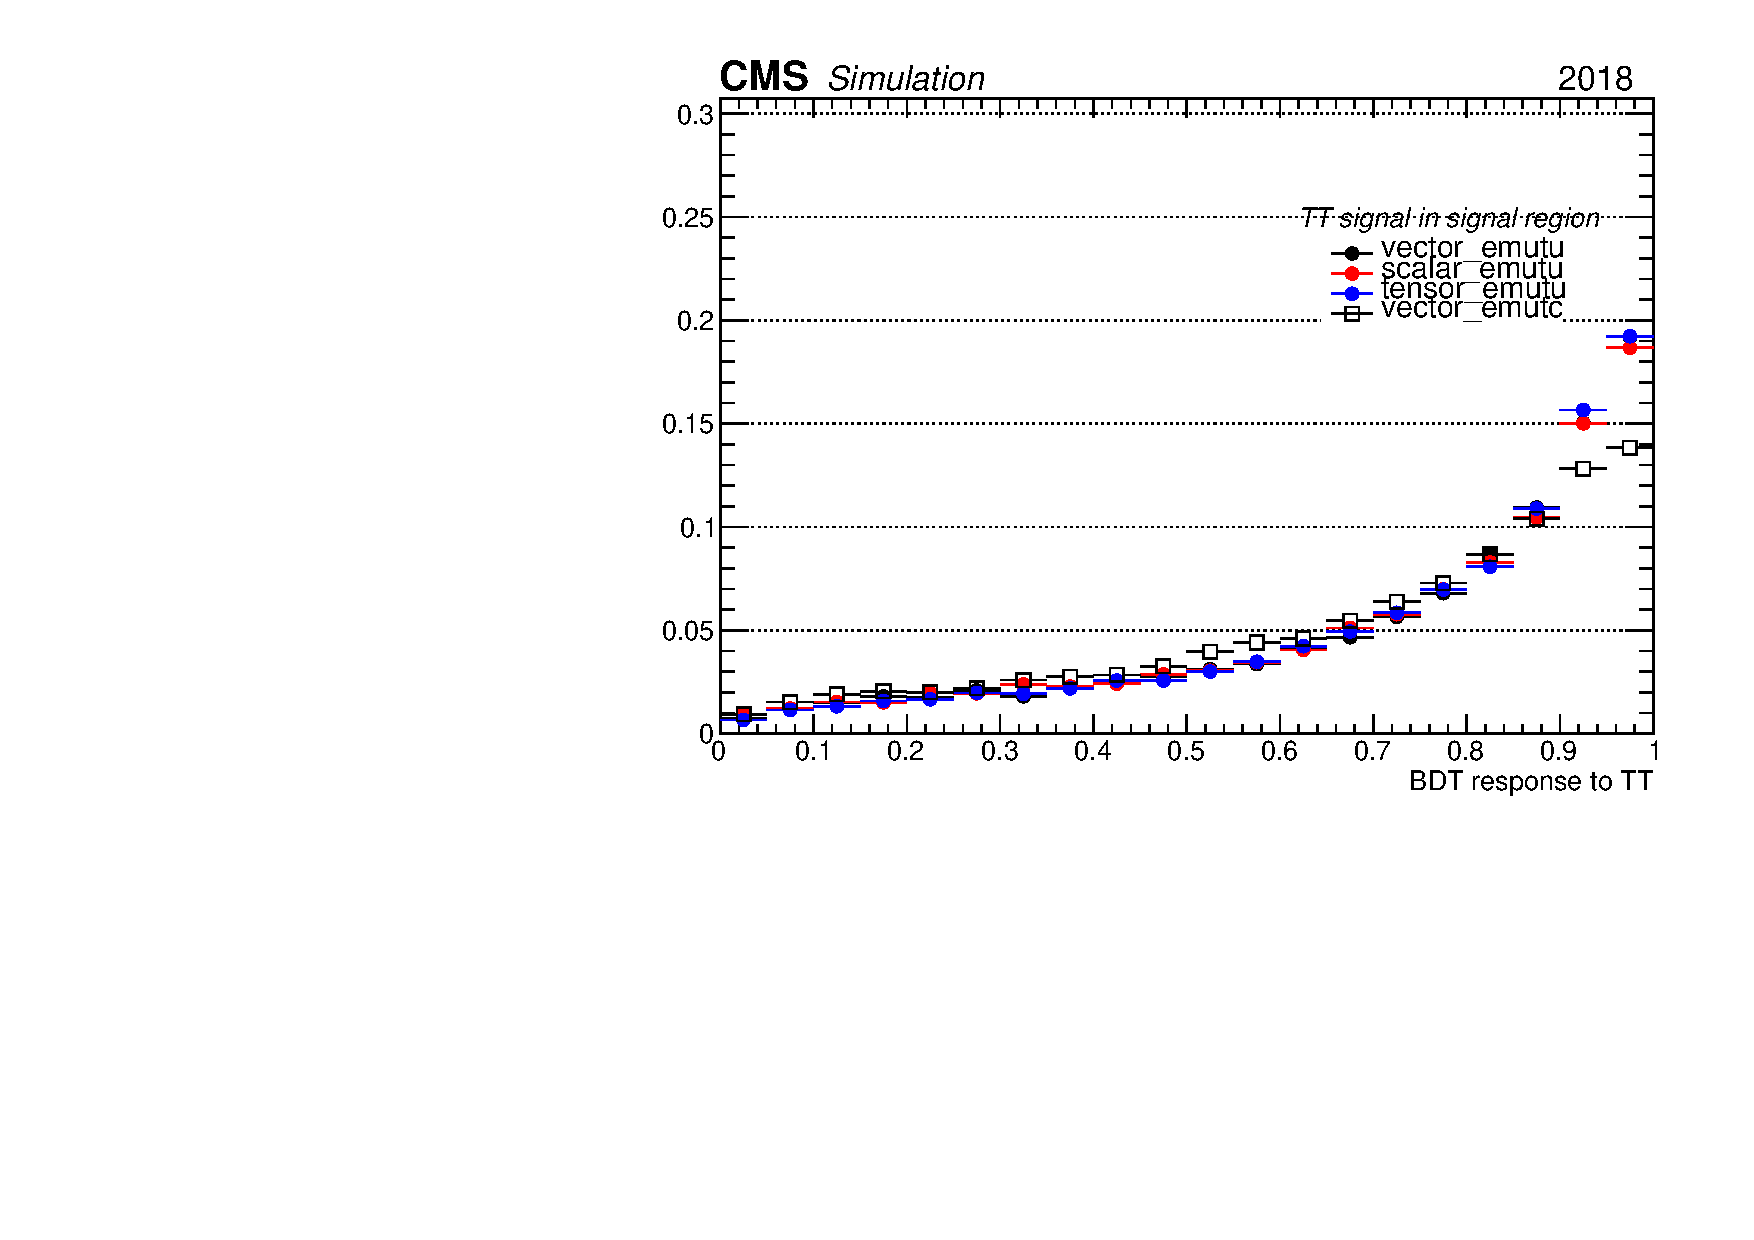
\includegraphics[width=0.48\textwidth]{figures/Part3/BDT/LFV_VR_emul_lllOffZMetg20Jetgeq1Bleq1_BDT_TT_N}\\
 \end{tabular}
 \caption{Normalized distribution in SR1. From left to right: LFV top mass, BDT shape}
 \label{fig:Lorentz}
 \end{center}
\end{figure}

The \emph{prompt} background dataset is constructed by combining all \ac{MC} samples listed under the ``prompt'' category listed in Table~\ref{tab:MCsample}. Cross sections referenced Table~\ref{tab:MCsample} are directly used to normalise the \emph{prompt} backgrounds. The construction of the \emph{nonpeompt} background dataset is different since the \emph{nonprompt} backgrounds are modelled with the \mm, which is itself constructed from 8 \acp{AR}. Therefore, 8 \acp{AR} are constructed to collect simulated $\ttbar$ and Drell-Yan events. These events used to form the \emph{nonprompt} dataset. Each event in the \emph{nonprompt} dataset is then ``weighted'' using the output of the \mm. Finally, the \emph{nonprompt} dataset is combined with the \emph{prompt} dataset and then divided into to datasets using a 150 GeV threshold on LFV e$\upmu$ mass. 

A technique know as the ``$k$-fold cross validation'' is used to minimise the loss of statistics when partitioning datasets into training, validation, and test sets. For each targeted \ac{SR}, the corresponding signal/background set is divided evenly into five subsets. Three out of the five subsets are used in the training while a fourth subset is used as a validation set. The fifth set is used to test the performance of the trained \ac{BDT}. A second \ac{BDT} is trained using a different combination of subsets to form training, validation, and test sets. This process is repeated five times until a unique test set no longer exists, which is illustrated in Figure~\ref{fig:5fold}. This technique ensures that the test set is always statistically independent of the process of parameters tuning, which serves as the basis for the bias-free evaluation after training: when evaluating each event using the trained model, it is always possible to pick one of the five \acp{BDT} where this particular event was not included in the training or validation.

\begin{figure}[tbh!]
 \begin{center}
   \caption{Illustration of a 5-fold cross validation.}
 \begin{tabular}{c}
  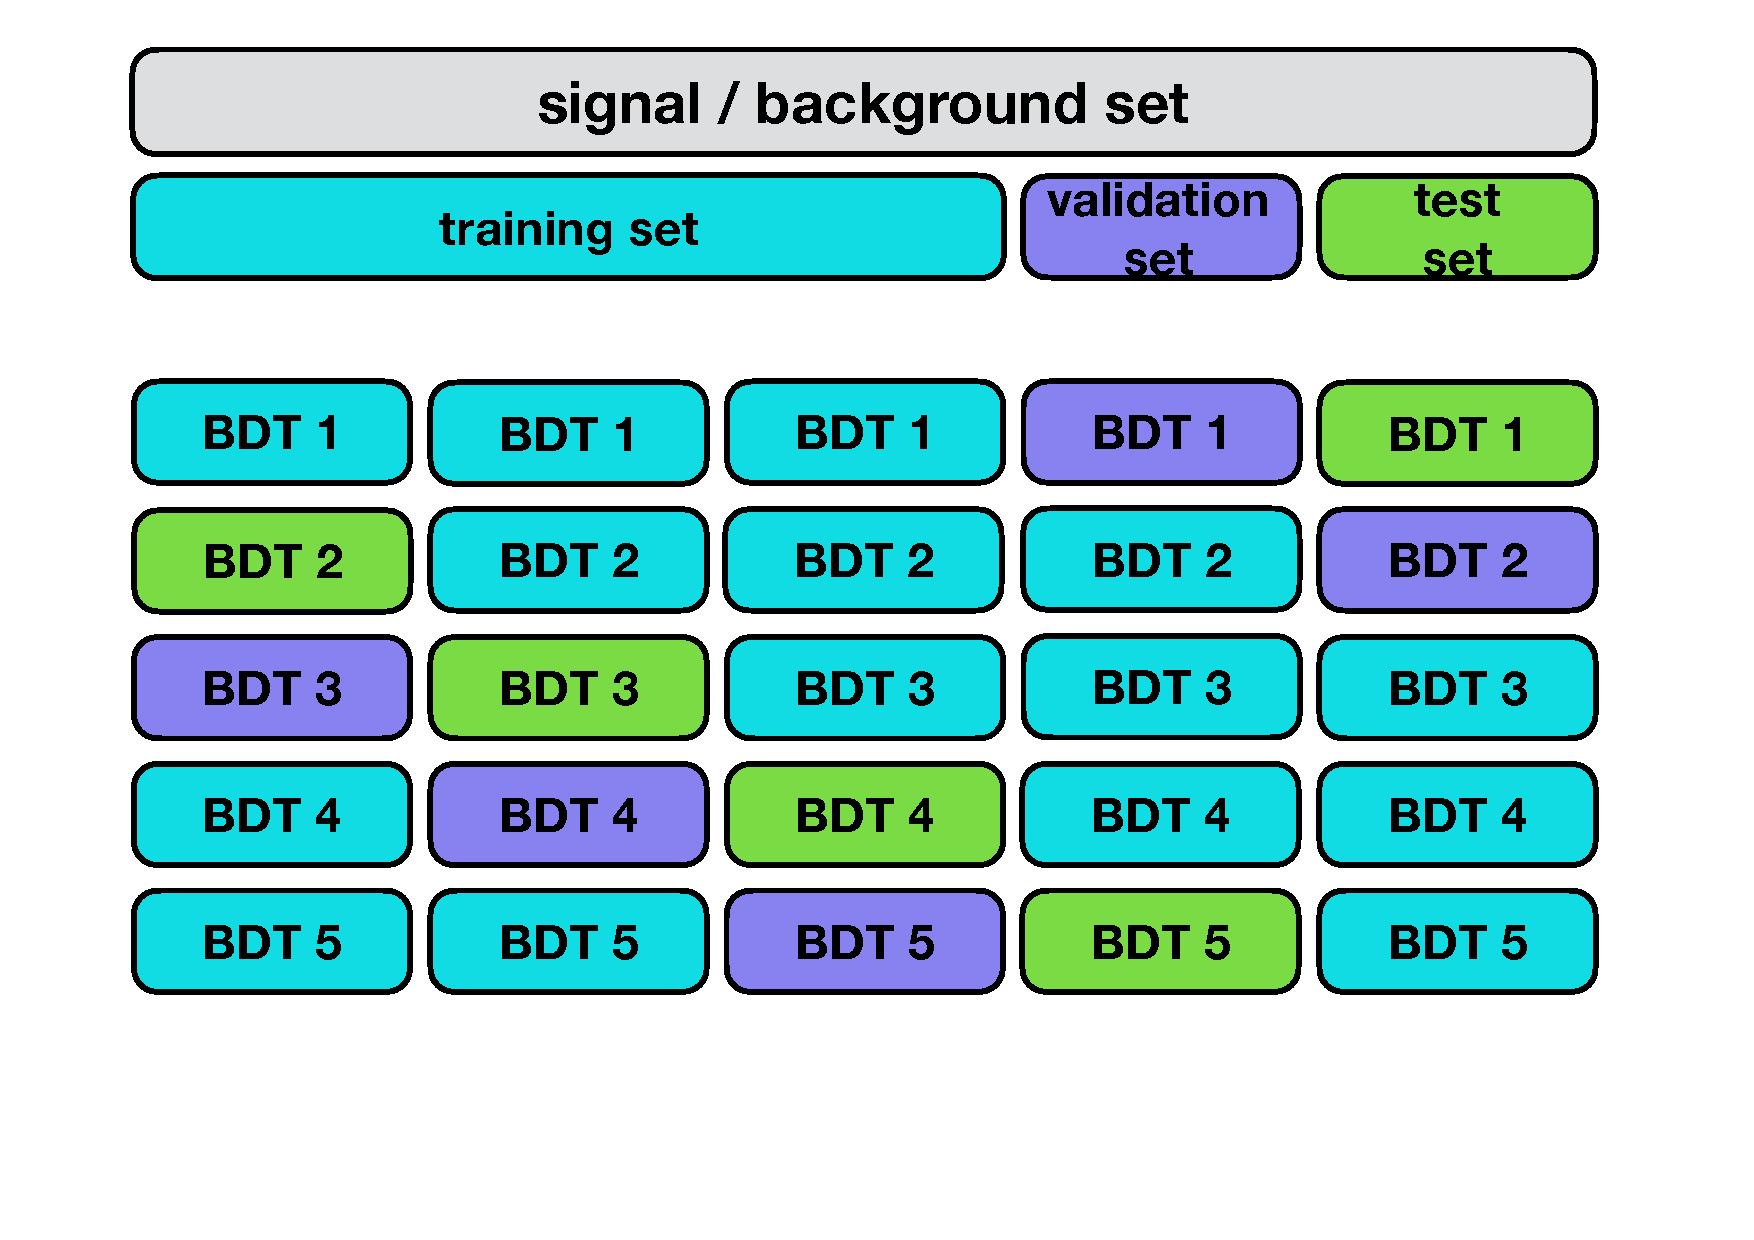
\includegraphics[width=0.8\textwidth]{figures/Part3/BDT/kfold}
 \end{tabular}
 \label{fig:5fold}
 \end{center}
\end{figure}

The same set of hyper parameters are used for all \acp{BDT}, which are optimised using a randomised grid search algorithm. The number of estimators is set to 1000 with a max depth of 5. Standard loss function implemented in \cite{Chen:2016:XST:2939672.2939785} is uses as the evaluation metric. The performance of the \ac{BDT} is visualised using a metric known as ``\ac{ROC}'', which is shown in Figure \ref{fig:5fold}. In general, the \acp{BDT} trained in  \ac{SR}2 (i.e. $\textsf{m}_{\textsf{e}\upmu}~>$ 150 GeV) are much more performant due to the high $\pt$ objects in the final states.

\begin{figure}[tbh!]
 \begin{center}
 \begin{tabular}{cc}
  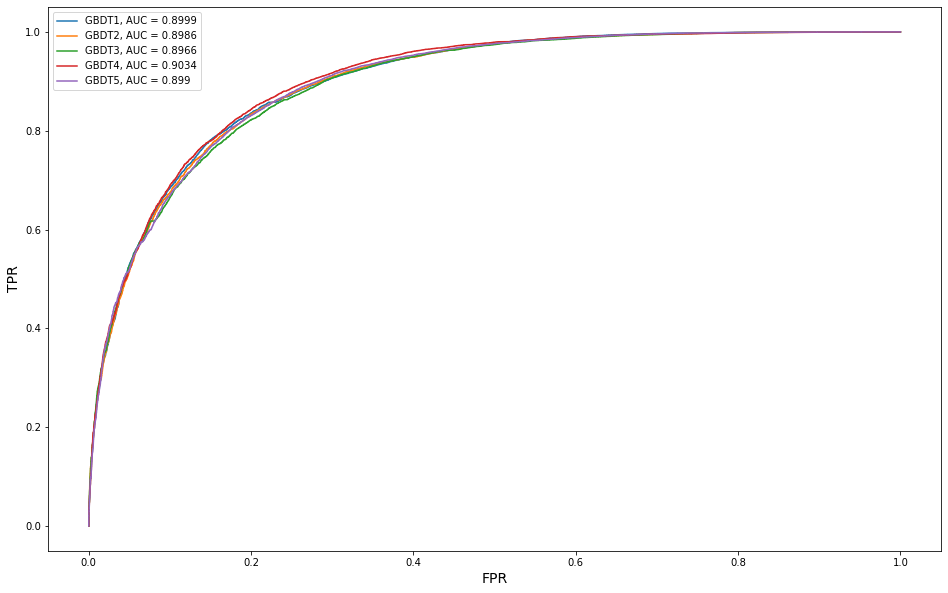
\includegraphics[width=0.48\textwidth]{figures/Part3/BDT/5foldTT}&
    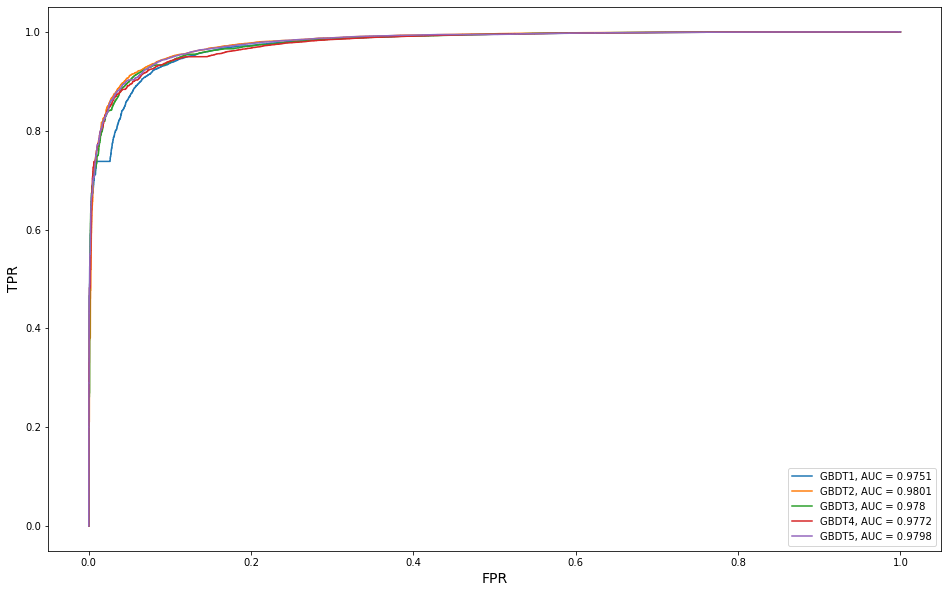
\includegraphics[width=0.48\textwidth]{figures/Part3/BDT/5foldST}\\
 \end{tabular}
 \caption{ROC curve with 5-fold cross validation. From left to right: BDT targeting TT (SR1), BDT targeting ST (SR2).}
 \label{fig:ROC}
 \end{center}
\end{figure}
%%%%%%%%%%%%%%%%%%%%%%%%%%%%%%%%%%%%%%%%%%%%%%%%%%%%%%%%%%
%%%%%%%%%%%%%%%%%%%%%%%%%%%%%%%%%%%%%%%%%%%%%%%%%%%%%%%%%%

\section{BDT Features}
\label{sec:Input}

The observables used in training are referred to as "features" in this analysis. The following features are used for both ST and TT classifier:

\begin{itemize}
\item \textbf{MVA\_M$_{e\mu}$: invariant mass of the Opposite-Sign $e\mu$ pair}
\item \textbf{MVA\_LFVePt: $p_T$ of the flavor-violating electron}
\item \textbf{MVA\_LFVmuPt: $p_T$ of the flavor-violating muon}
\item \textbf{MVA\_LFVTopmass: invariant mass of the flavor-violating top-quark candidate}
\item \textbf{MVA\_Zmass: invariant mass of Z boson candidate}
\item \textbf{MVA\_Jet2Btag: b-tagging score of the jet with the second highest b-tagging score}
\item \textbf{MVA\_Mbl2: invariant mass of the second b-jet+lepton system}
\item \textbf{MVA\_njet: number of jets}
\item \textbf{MVA\_nbjet: number of b-jets}
\item \textbf{MVA\_tM: transverse mass of the W boson candidate (from standard model top-quark)}
\item \textbf{MVA\_llDr: $\Delta R$ between flavor-violating electron and muon}
\item \textbf{MVA\_SSee\_Zmass: invariant mass of a Same-Sign di-electron pair}
\item \textbf{MVA\_Topmass: invariant mass of the standard model top-quark candidate}
\item \textbf{MVA\_Met: missing transverse energy}
\end{itemize}

The following features are only used for TT classifier:

\begin{itemize}
\item \textbf{MVA\_Ht: scalar sum of the $p_T$ of all objects}
\item \textbf{MVA\_Mbl1: invariant mass of the second bjet+lepton system}
\item \textbf{MVA\_JeDr: $\Delta R$ between flavor-violating electron and a light jet (non-b-jet)}
\item \textbf{MVA\_JmuDr: $\Delta R$ between flavor-violating muon and a light jet (non-b-jet)}
\end{itemize}

The following features are used for ST classifier:

\begin{itemize}
\item \textbf{MVA\_BaPt: $p_T$ of the standard model lepton}
\item \textbf{MVA\_JetHt: scalar sum of the $p_T$ of jets}
\end{itemize}

Distributions of selected features are shown in Figure \ref{fig:Features1}-\ref{fig:Features5}.

\begin{figure}[tbh!]
 \begin{center}
 \begin{tabular}{c}
  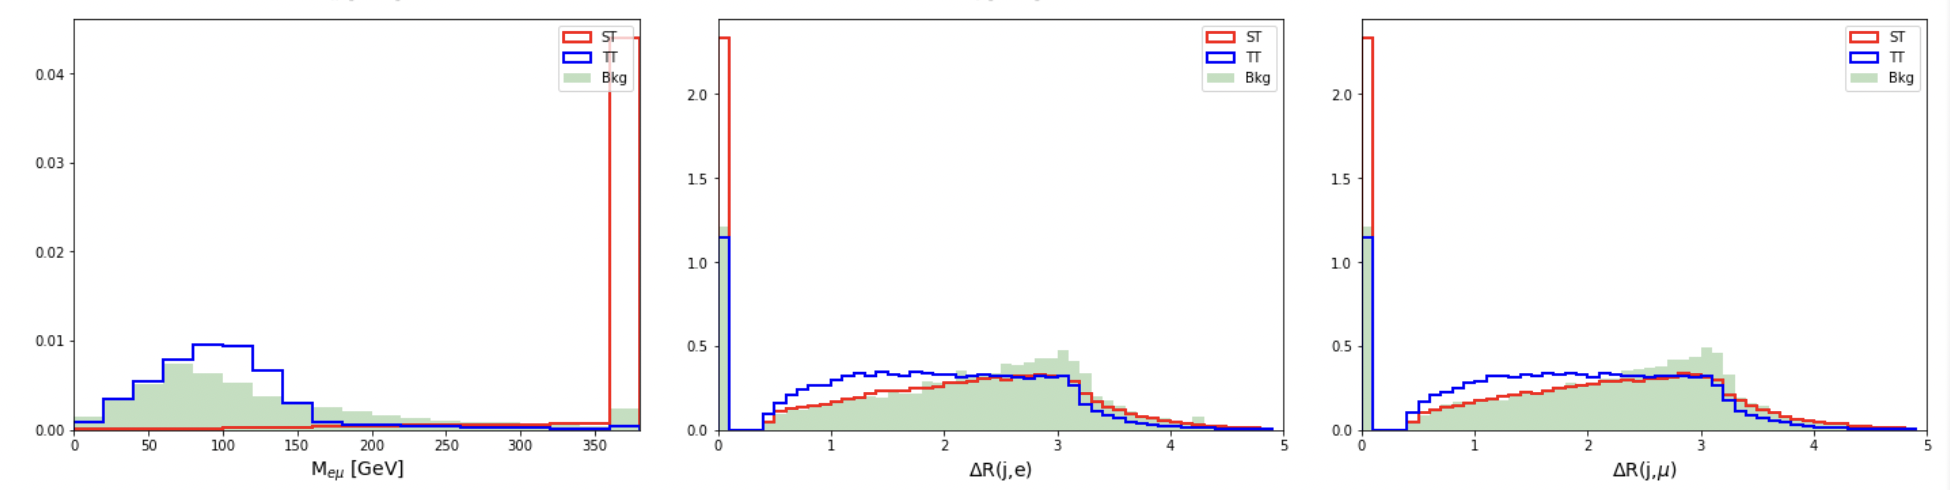
\includegraphics[width=0.99\textwidth]{figures/Part3/BDT/Features1}\\
 \end{tabular}
 \caption{Normalized distribution of various features in SR. From to left to right: MVA\_M$_{e\mu}$, MVA\_JeDr, MVA\_JeDr.}
 \label{fig:Features1}
 \end{center}
\end{figure}

\begin{figure}[tbh!]
 \begin{center}
 \begin{tabular}{c}
  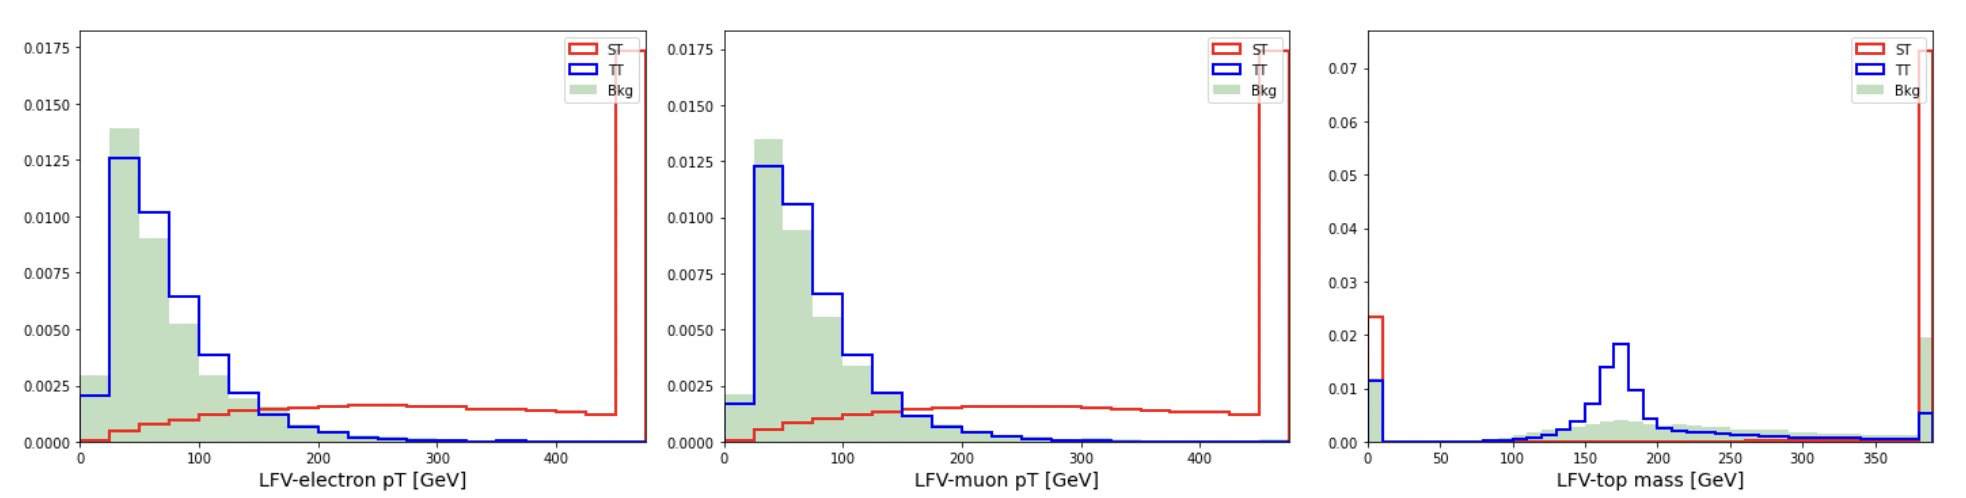
\includegraphics[width=0.99\textwidth]{figures/Part3/BDT/Features2}\\
 \end{tabular}
 \caption{Normalized distribution of additional features in SR. From to left to right: MVA\_LFVePt, MVA\_LFVmuPt, MVA\_LFVTopmass.}
 \label{fig:Features2}
 \end{center}
\end{figure}

\begin{figure}[tbh!]
 \begin{center}
 \begin{tabular}{c}
  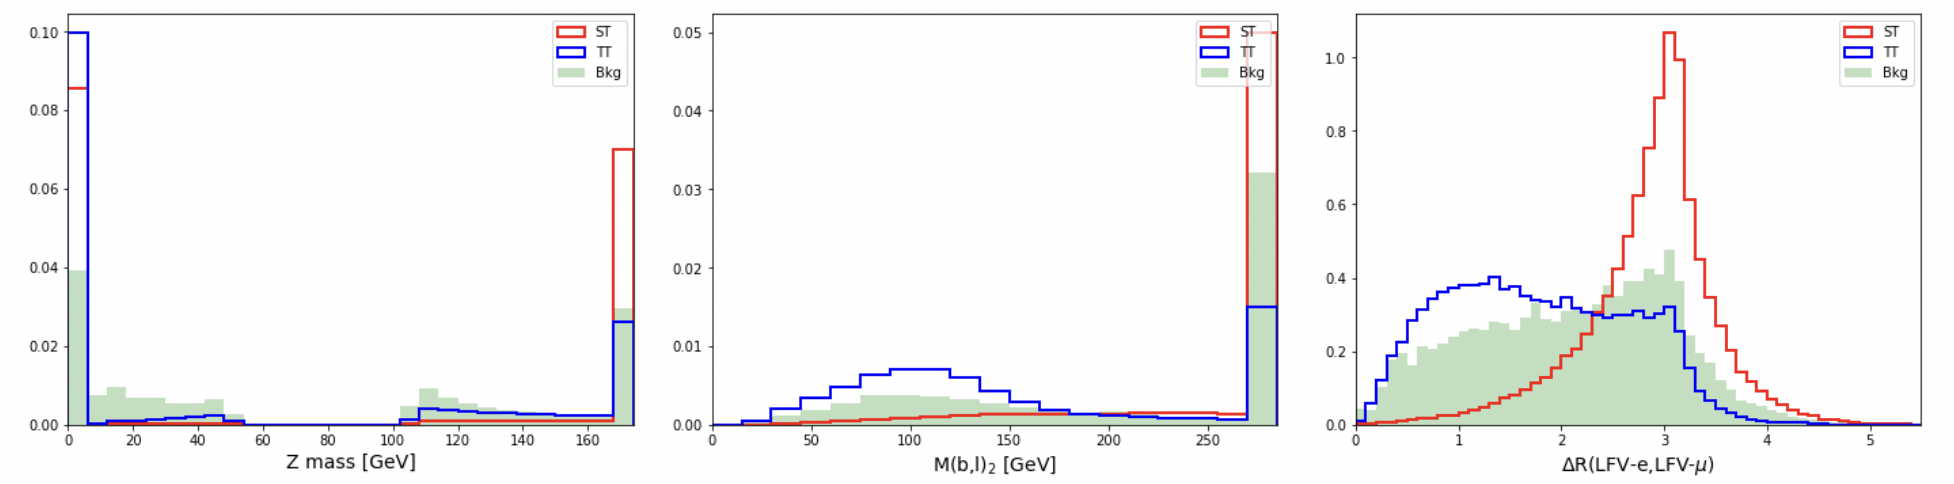
\includegraphics[width=0.99\textwidth]{figures/Part3/BDT/Features3}\\
 \end{tabular}
 \caption{Normalized distribution of additional features in SR. From to left to right: MVA\_Zmass, MVA\_Mbl2, MVA\_llDr.}
 \label{fig:Features3}
 \end{center}
\end{figure}

\begin{figure}[tbh!]
 \begin{center}
 \begin{tabular}{c}
  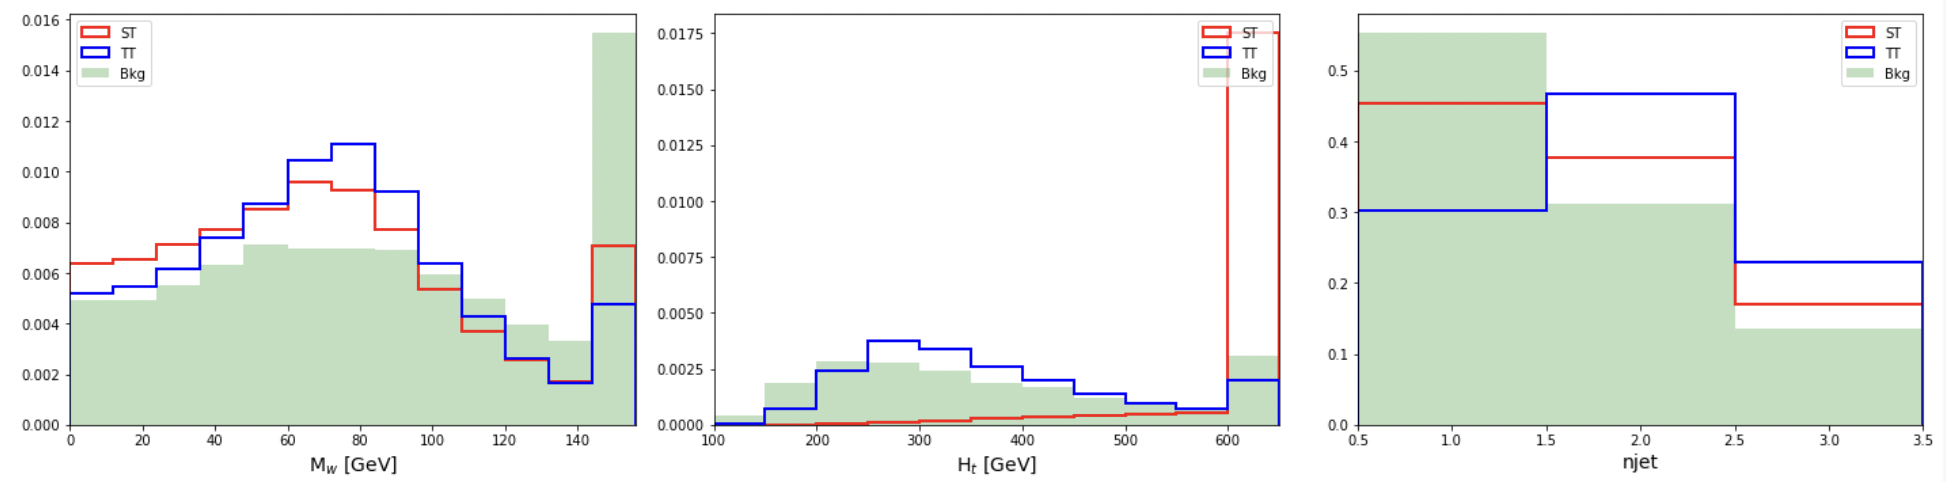
\includegraphics[width=0.99\textwidth]{figures/Part3/BDT/Features4}\\
 \end{tabular}
 \caption{Normalized distribution of additional features in SR. From to left to right: MVA\_tM, MVA\_Ht, MVA\_njet.}
 \label{fig:Features4}
 \end{center}
\end{figure}

\begin{figure}[tbh!]
 \begin{center}
 \begin{tabular}{c}
  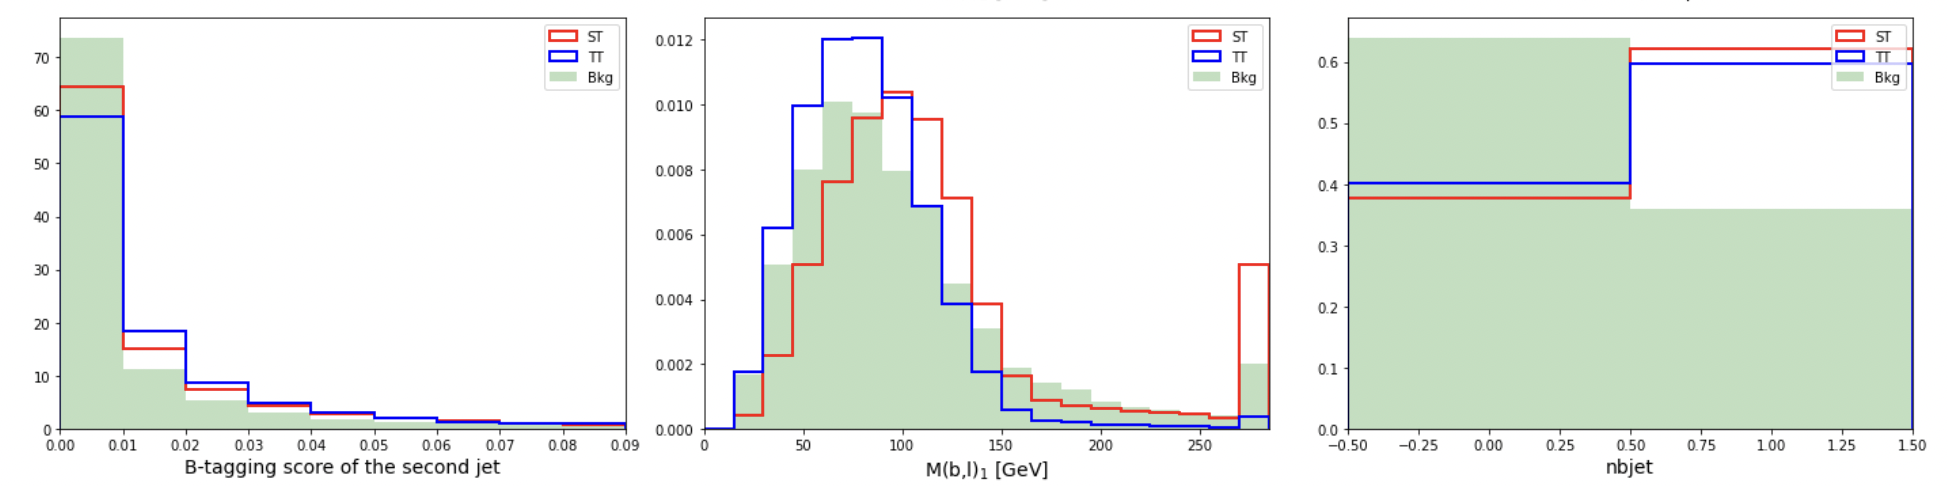
\includegraphics[width=0.99\textwidth]{figures/Part3/BDT/Features5}\\
 \end{tabular}
 \caption{Normalized distribution of additional features in SR. From to left to right: MVA\_Jet2Btag, MVA\_Mbl1, MVA\_nbjet.}
 \label{fig:Features5}
 \end{center}
\end{figure}

To determine the relative importance of these features, feature importance is extracted using the "gain" method and is shown in Figure \ref{fig:Ranking}.

\begin{figure}[tbh!]
 \begin{center}
 \begin{tabular}{cc}
  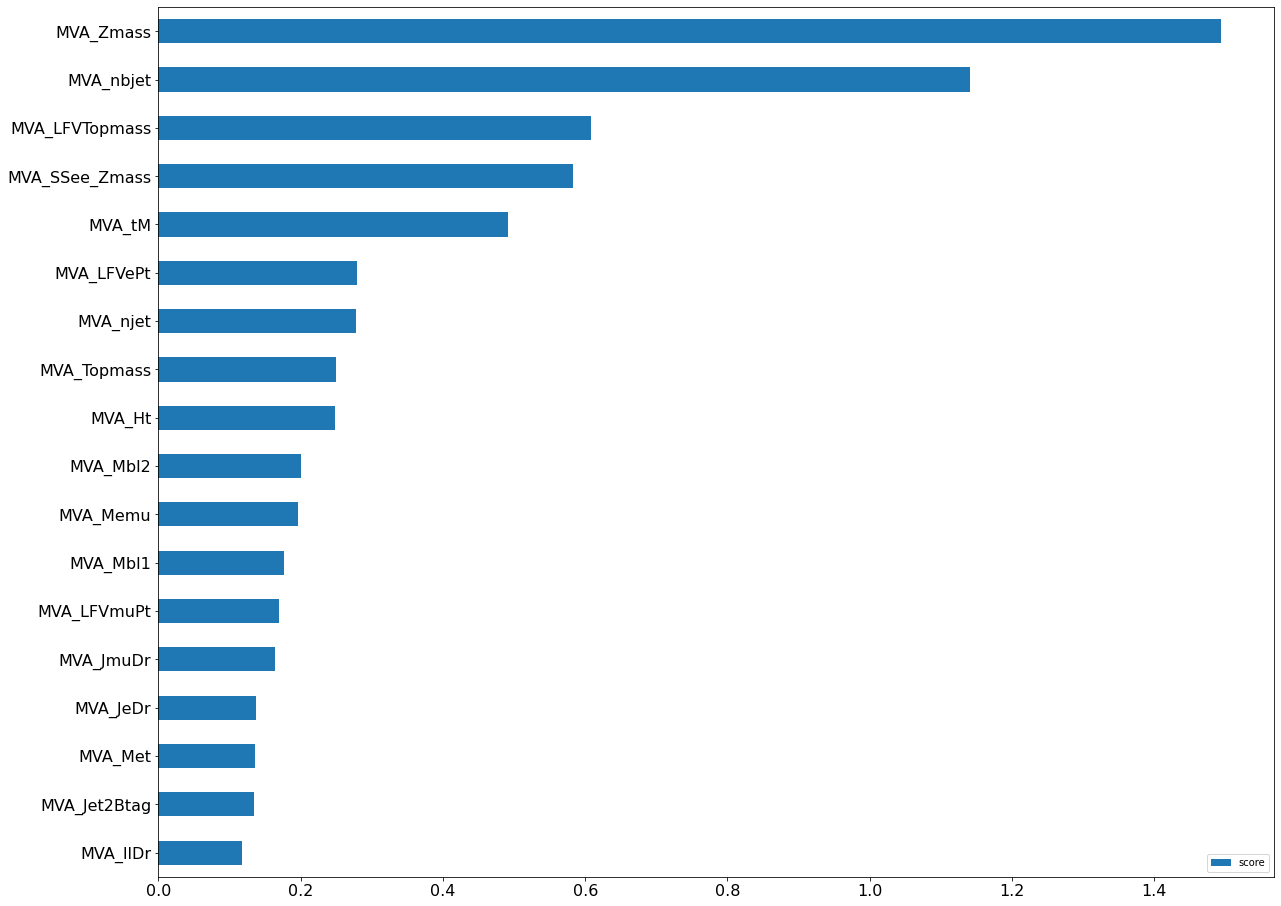
\includegraphics[width=0.48\textwidth]{figures/Part3/BDT/TTranking}&
  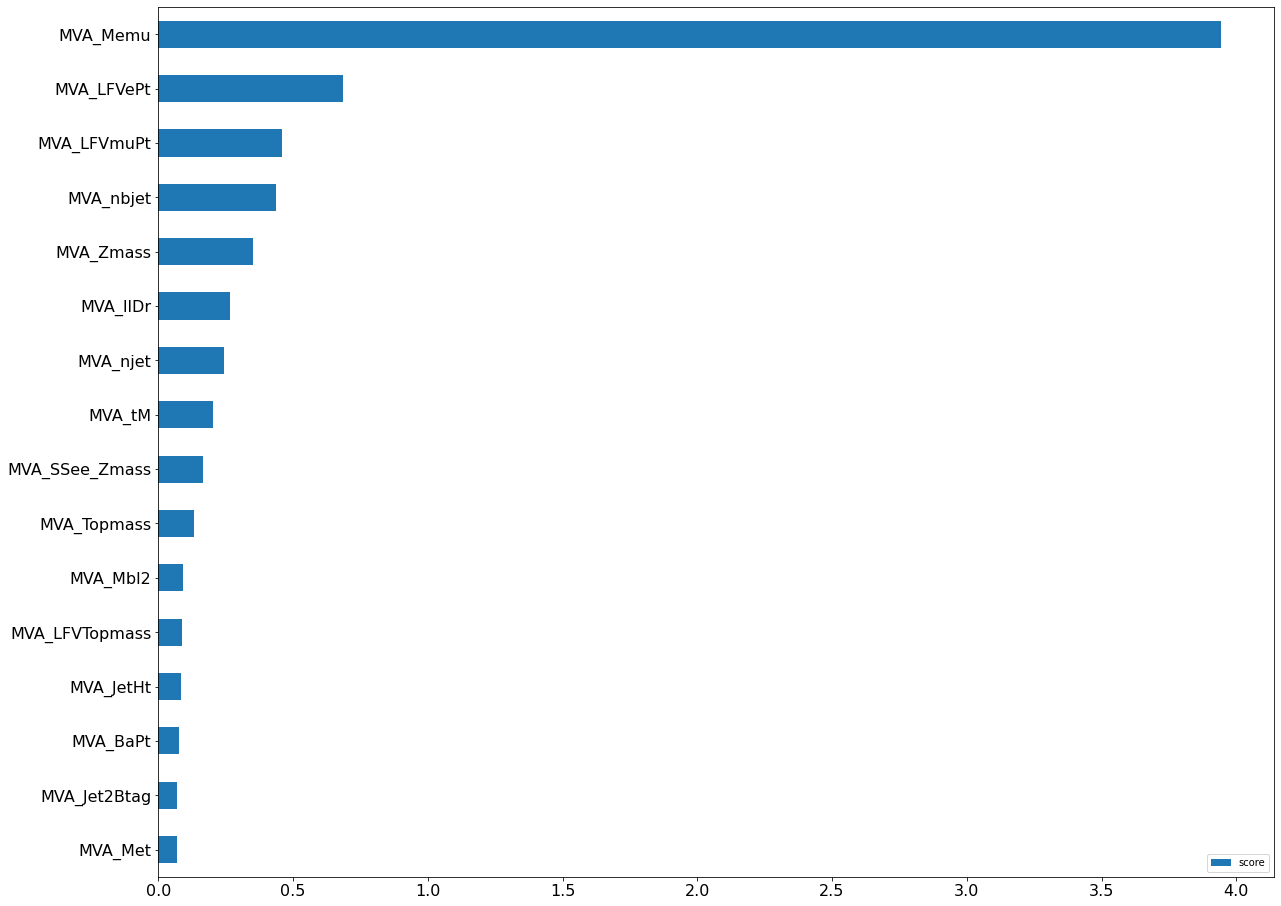
\includegraphics[width=0.48\textwidth]{figures/Part3/BDT/STranking}\\
 \end{tabular}
 \caption{List of features ranked by their relative importance. From left to right: BDT targeting TT (SR1), BDT targeting ST (SR2)}
 \label{fig:Ranking}
 \end{center}
\end{figure}

\begin{figure}[tbh!]
 \begin{center}
 \begin{tabular}{cc}
  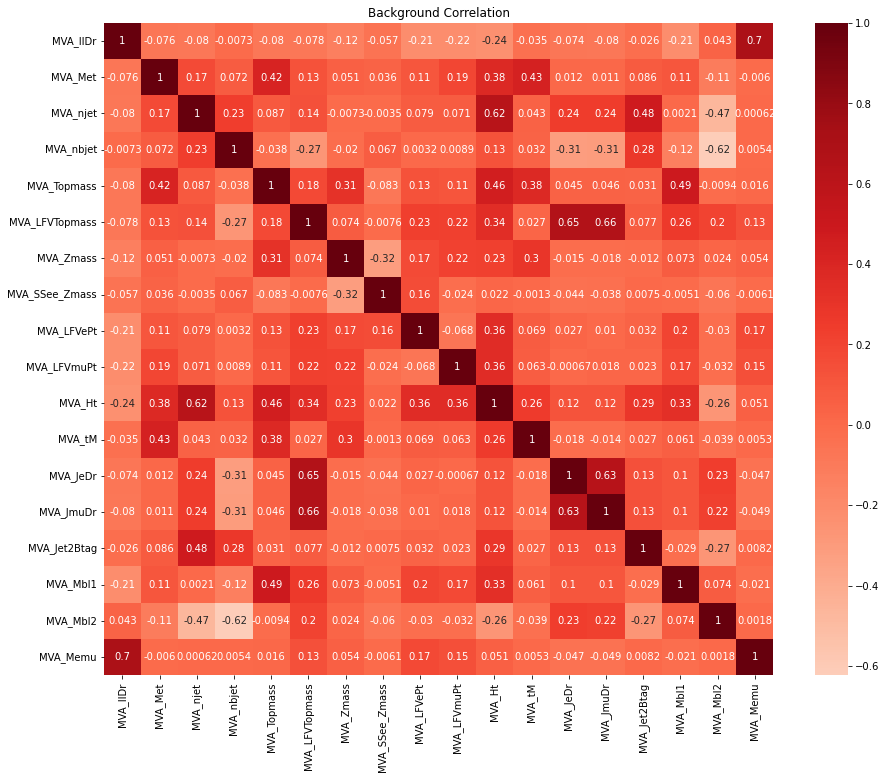
\includegraphics[width=0.48\textwidth]{figures/Part3/BDT/corr_bkg_SR1}&
  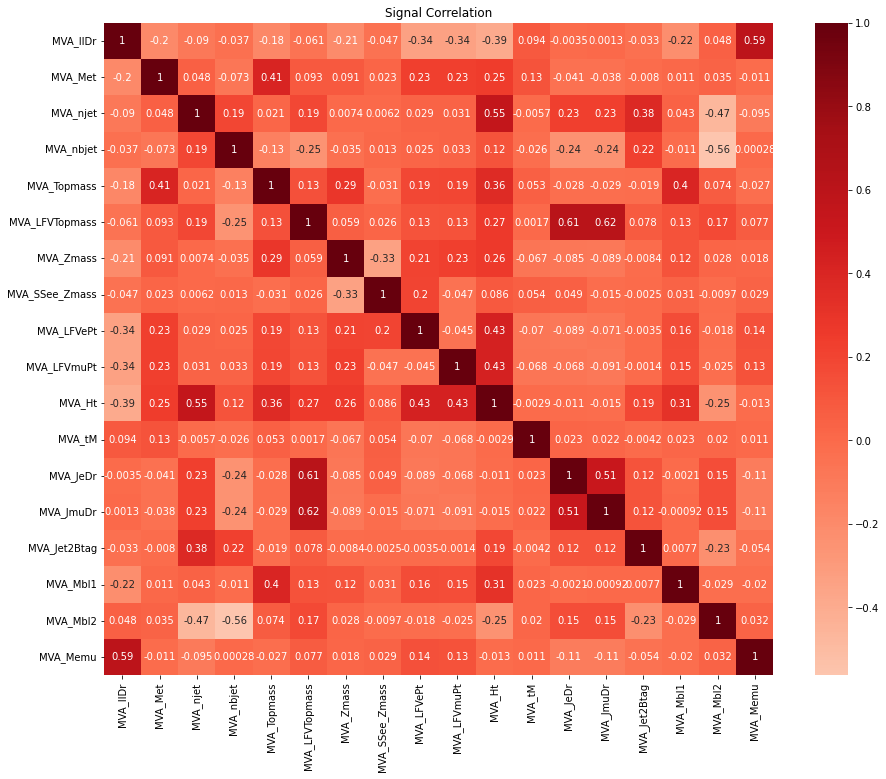
\includegraphics[width=0.48\textwidth]{figures/Part3/BDT/corr_signal_SR1}\\
 \end{tabular}
 \caption{Correlation matrices (SR1), from left to right: background correlation, signal correlation.}
 \label{fig:Ranking}
 \end{center}
\end{figure}

\begin{figure}[tbh!]
 \begin{center}
 \begin{tabular}{cc}
  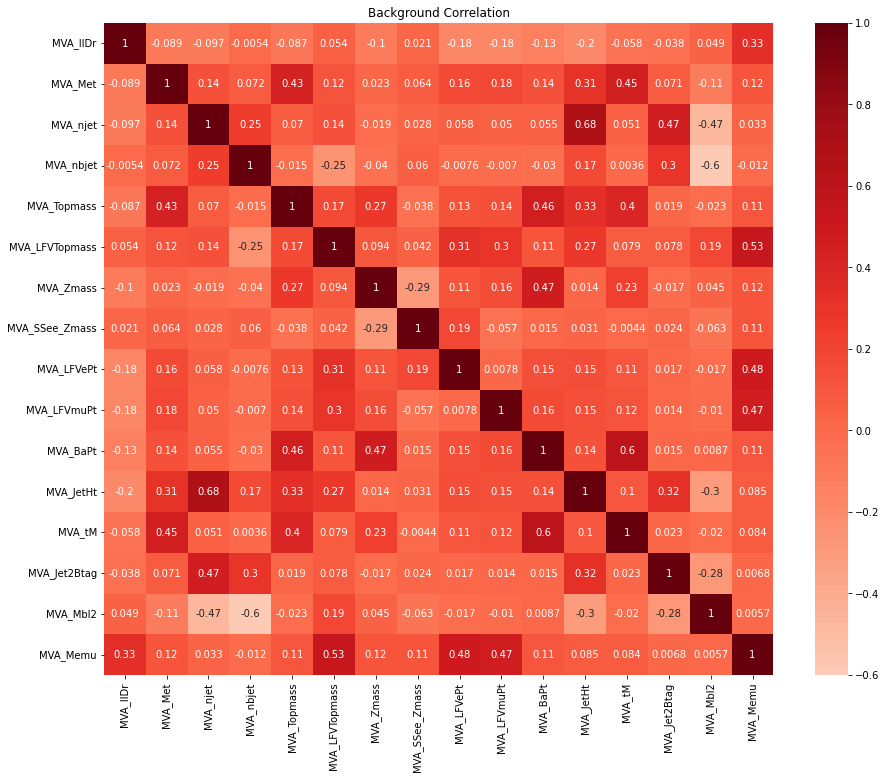
\includegraphics[width=0.48\textwidth]{figures/Part3/BDT/corr_bkg_SR2}&
  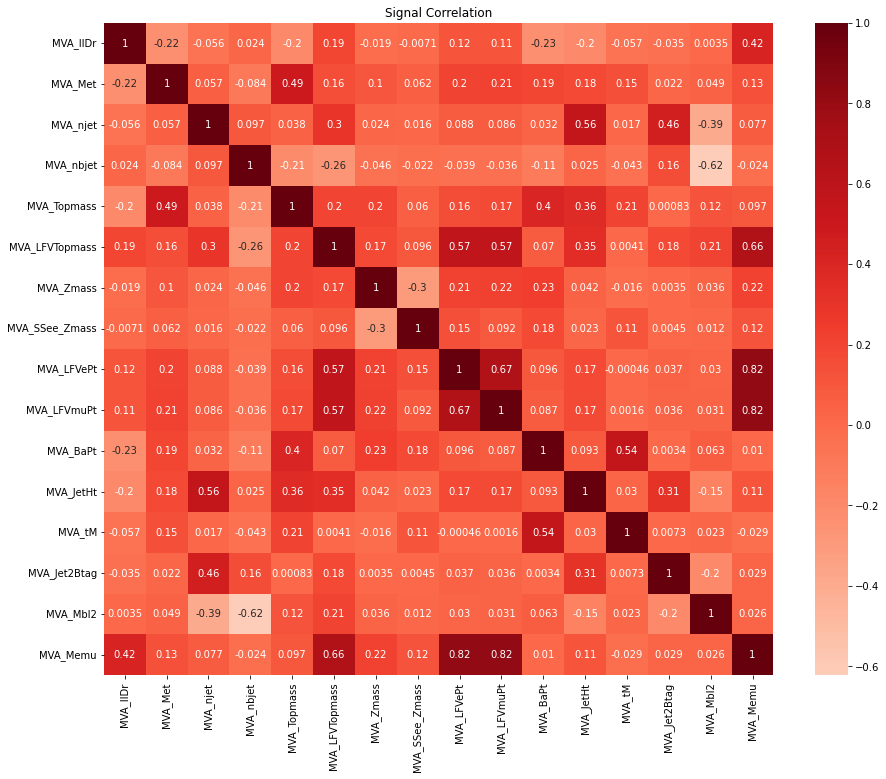
\includegraphics[width=0.48\textwidth]{figures/Part3/BDT/corr_signal_SR2}\\
 \end{tabular}
 \caption{Correlation matrices (SR2), from left to right: background correlation, signal correlation.}
 \label{fig:Ranking}
 \end{center}
\end{figure}
%%%%%%%%%%%%%%%%%%%%%%%%%%%%%%%%%%%%%%%%%%%%%%%%%%%%%%%%%%
%%%%%%%%%%%%%%%%%%%%%%%%%%%%%%%%%%%%%%%%%%%%%%%%%%%%%%%%%%

\section{BDT Output}
\label{sec:Output}

The output of the BDTs are shown in Figure \ref{fig:bdt_output}. Note: all but the nonprompt backgrounds are estimated with MC simulation. The nonprompt background backgrounds are estimated with the matrix method.

\begin{figure}[tbh!]
 \begin{center}
 \begin{tabular}{cc}
  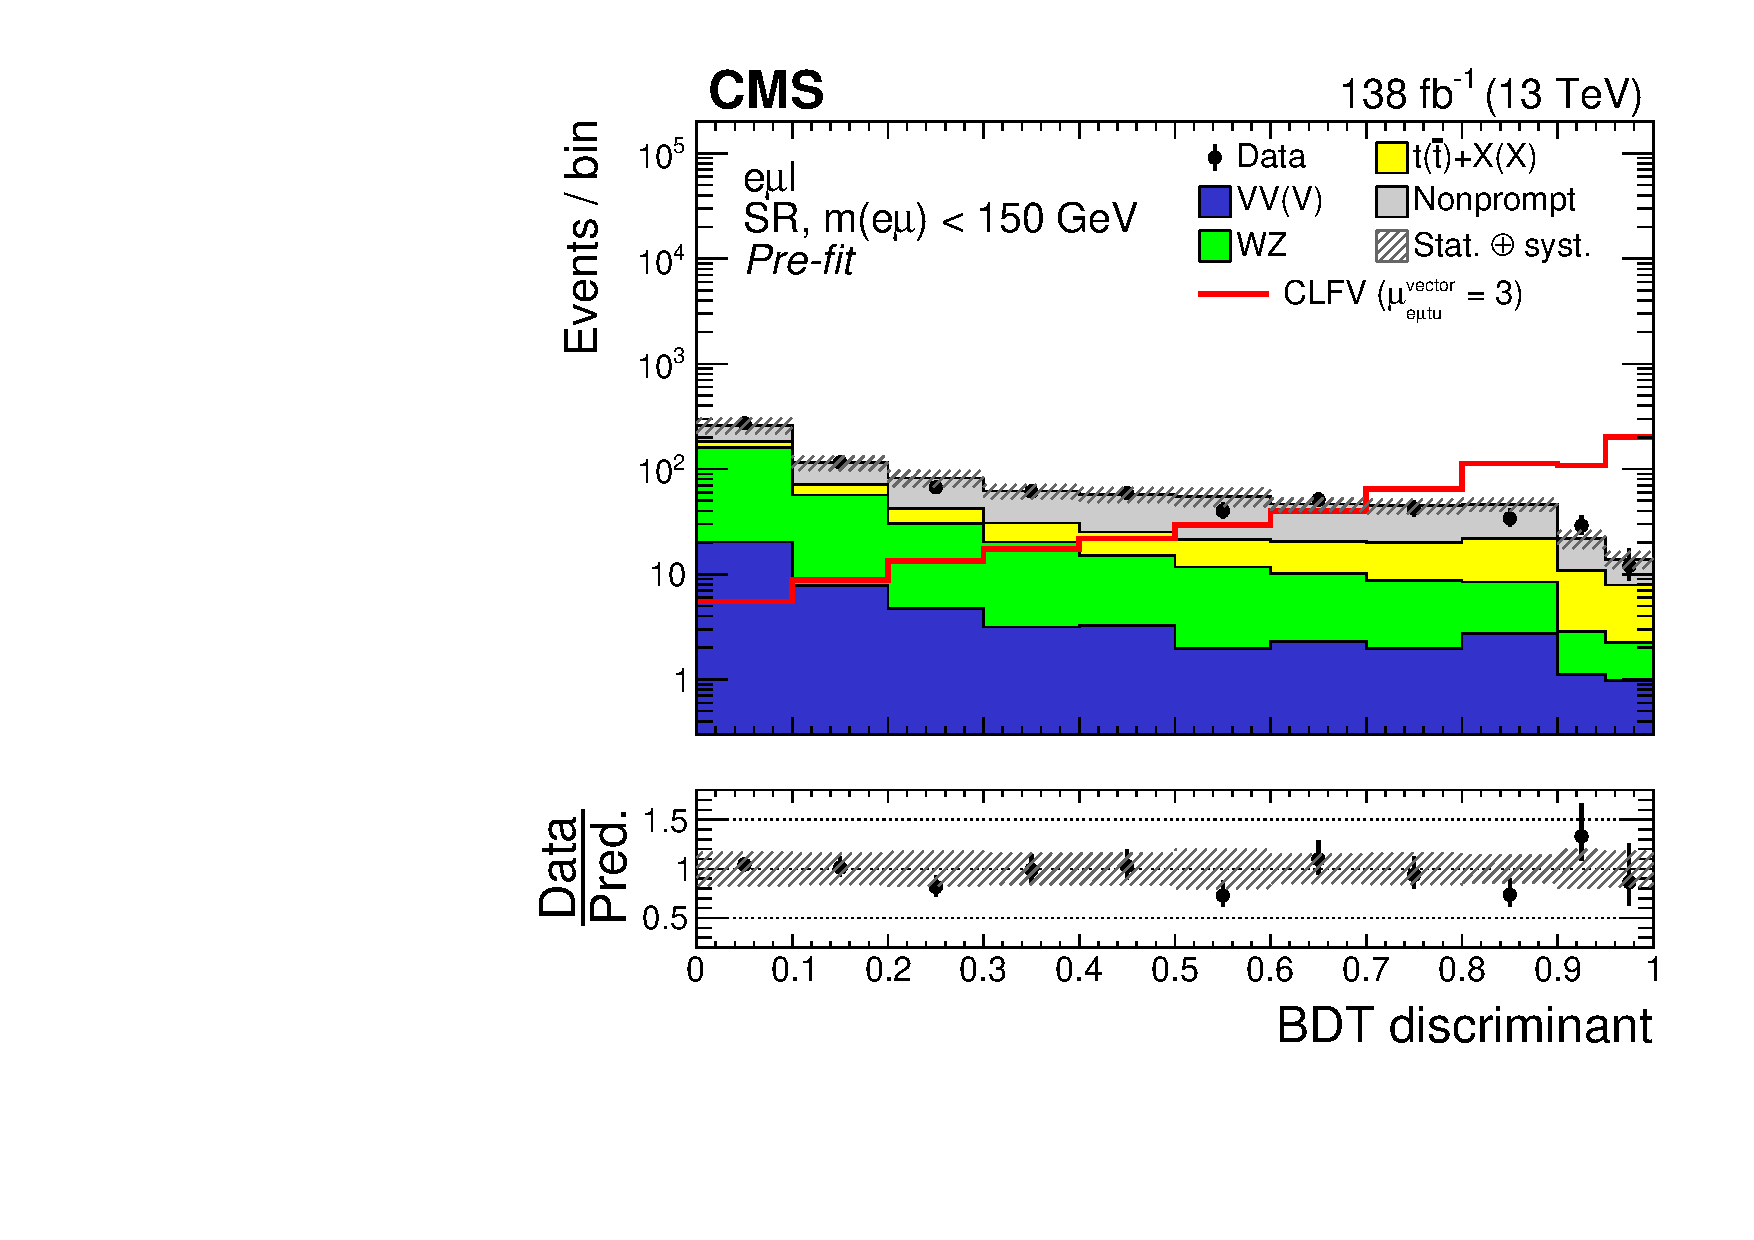
\includegraphics[width=0.48\textwidth]{figures/Part3/BDT/BDT_TT}&
  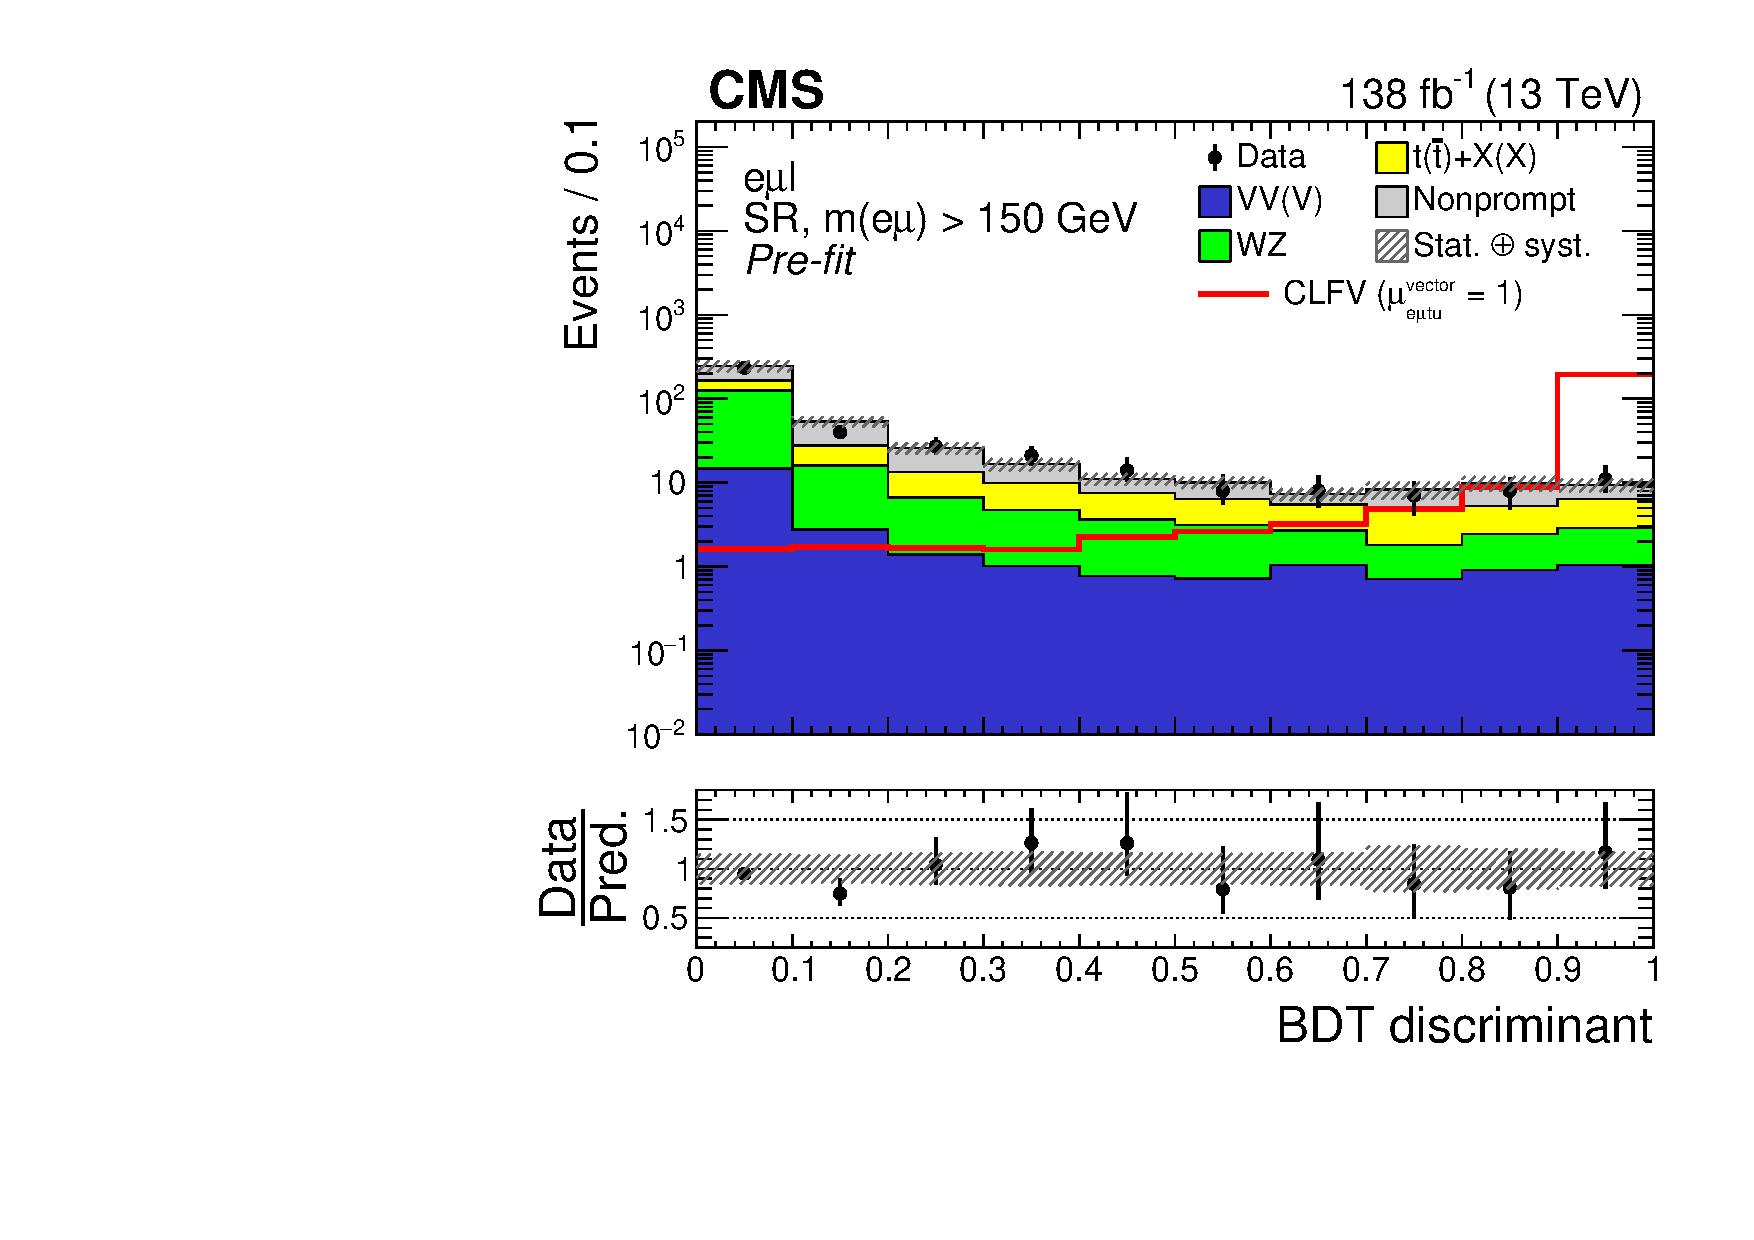
\includegraphics[width=0.48\textwidth]{figures/Part3/BDT/BDT_ST}\\
 \end{tabular}
 \caption{Distribution of BDT output, from left to right TT enriched SR (SR1), ST enriched SR (SR2)}
 \label{fig:bdt_output}
 \end{center}
\end{figure}
\chapter{Systematic Uncertainties}
\label{chap:Systematics}

Different sources of systematic uncertainty contribute to the estimation of background events and modeling of the signal. The chapter is organized as follows. Theoretical uncertainties concerning signals and major backgrounds are discussed in \autoref{sec:ThUnc}. Uncertainties concerning the \emph{nonprompt} background is discussed in \autoref{sec:NonUnc}. Uncertainties concerning the modeling of the diboson processes are discribed in \autoref{sec:DiUnc}. Finally, other systematic uncertainties are discussed in \autoref{sec:OthUnc}.
%%%%%%%%%%%%%%%%%%%%%%%%%%%%%%%%%%%%%%%%%%%%%%%%%%%%%%%%
%%%%%%%%%%%%%%%%%%%%%%%%%%%%%%%%%%%%%%%%%%%%%%%%%%%%%%%%

\section{Theoretical Uncertainties}
\label{sec:ThUnc}

Variations on theoretical cross sections for \emph{prompt} backgrounds are introduced to cover the uncertainties in perturbative \ac{QCD} calculations.  A 6$\%$ normalization uncertainty is assigned to WZ and ZZ processes~\cite{Campbell:2011bn}. A 15$\%$ normalization uncertainty is assigned to $\ttbar$W, $\ttbar$Z, and $\ttbar$H processes~\cite{Frederix:2021agh,Kulesza:2020nfh}. A 20$\%$ normalization uncertainty is assigned to tZq process, which is a conservative estimate taken from the MC generator. A conservative 50 $\%$ normalization uncertainty is assigned to other smaller \emph{prompt} backgrounds. All normalization uncertainties are considered uncorrelated between different processes but correlated between the years. 

Uncertainties associated to the \ac{PDF} are evaluated by using 100 replicas of the NNPDF sets~\cite{NNPDF:2014otw,NNPDF:2017mvq}. The procedure described in~\cite{CMS:2012nsv} is followed. Firstly, the sum of the generator weights of each replica is normalized to the nominal sum of the generator weights. This is done before any event selection to ensure no addtional normalization effect is introduced. After previous step, the bin-by-bin variations of the \ac{BDT} templates are obtained by calculating the bin-by-bin difference of the \ac{BDT} templates when switching from nominal \ac{PDF} to each \ac{PDF} replica. Finally, \ac{PDF} uncertainty for each bin is assigned by taking the root mean square value of the 100 variations of the corresponding bin. This uncertainty is treated as uncorrelated between different processes but correlated between the years.  We consider this uncertainty for all the signals and major prompt backgrounds (i.e. WZ, $\ttbar$W, $\ttbar$Z, and $\ttbar$H).

\ac{QCD} scale uncertainties are evaluated by varying the renormalization scale $\mu_\textsf{R}$ and factorization scales $\mu_\textsf{F}$ in \ac{ME}.  A total of six variations are considered: varying $\mu_\textsf{R}$ by a factor of 2 and 0.5, varying $\mu_\textsf{F}$ by a factor of 2 and 0.5, and varying $\mu_\textsf{R}$ and $\mu_\textsf{F}$ simultaneously by a factor of 2 and 0.5. Similar to PDF uncertainty, normalization effects of each variation is removed. An envelope that covers all six variations is used to represent the scale uncertainty. This uncertainty is treated as uncorrelated between different processes but correlated between the years. We consider this uncertainty for all the signals and major prompt backgrounds (i.e. WZ, $\ttbar$W, $\ttbar$Z, and $\ttbar$H).

Uncertainties associated to the \ac{PS} are evaluated by varying the renormalization scale $\mu_\textsf{R}$ in the initial and final state radiations, which effectively changes the strong coupling constant in the \ac{PS}. Similarly, $\mu_\textsf{R}$ is varied by a factor of 2 and 0.5, and normalization effects of each variation is removed. This uncertainty is treated as uncorrelated between different processes but correlated between the years.  We consider this uncertainty for all the signals and major prompt backgrounds (i.e. WZ, $\ttbar$W, $\ttbar$Z, and $\ttbar$H).
%%%%%%%%%%%%%%%%%%%%%%%%%%%%%%%%%%%%%%%%%%%%%%%%%%%%%%%%
%%%%%%%%%%%%%%%%%%%%%%%%%%%%%%%%%%%%%%%%%%%%%%%%%%%%%%%%

\section{Nonprompt Uncertainties}
\label{sec:NonUnc}

There are several sources of uncertainties associated to the determination of the \emph{nonprompt} efficiency $f$. One of these uncertainties comes from the estimate of \emph{prompt} contamination in \ac{MR}. As is discussed in \autoref{chap:Nonprompt}, \emph{prompt} backgrounds (estimated with \ac{MC}) are subtracted from total event yields measured in data. A flat 20 $\%$ uncertainty ($\alpha$ in Equation \ref{eq:f_eq}) is assigned to the event yields of the \emph{prompt} background and the resulting variation of $f$ is taken as the uncertainty.

\begin{equation}
f=\frac{n_{data}^{tag+tight}-(1+\alpha)n_{MC(prompt)}^{tag+tight}}{n_{data}^{tag+loose}-(1+\alpha)n_{MC(prompt)}^{tag+loose}}.
\label{eq:f_eq}
\end{equation}  

\begin{figure}[tbh!]
 \begin{center}
 \begin{tabular}{c}
 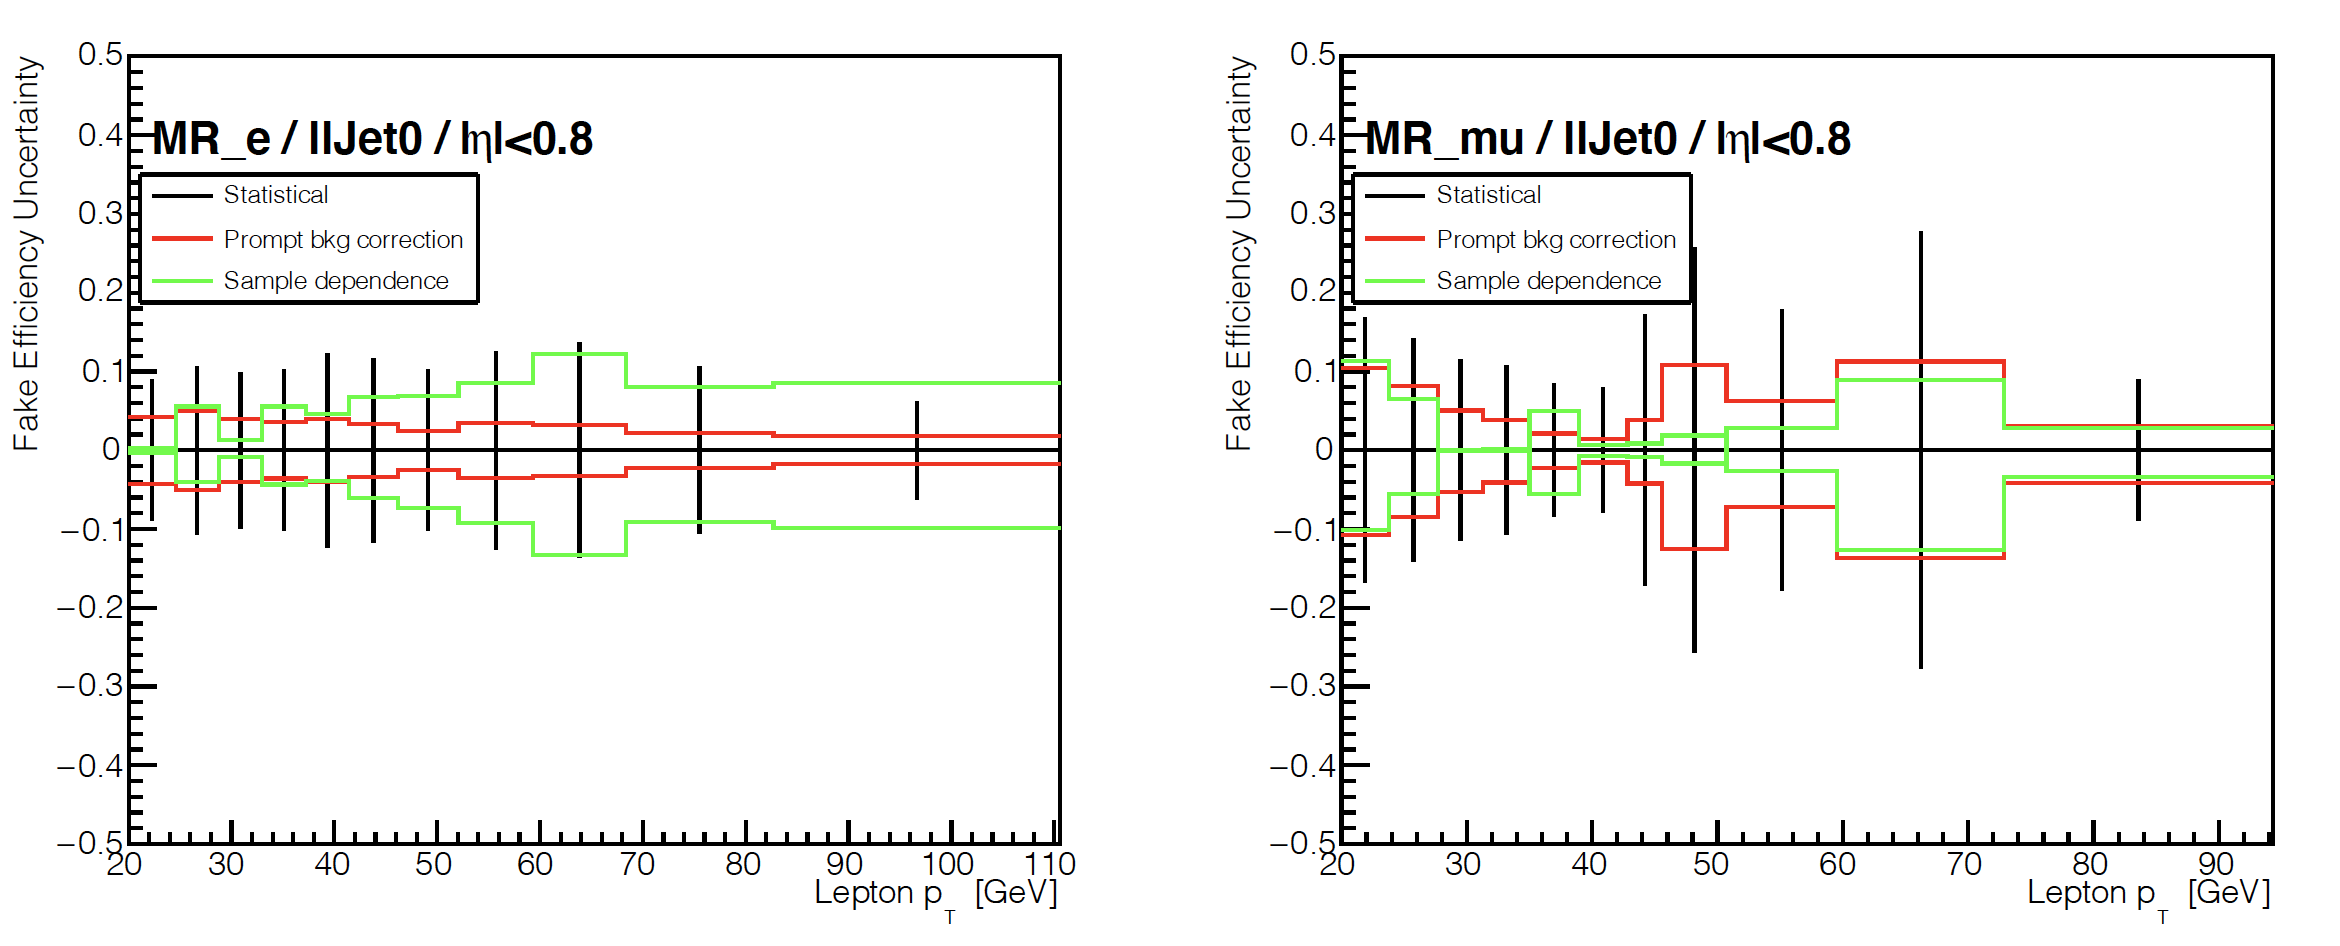
\includegraphics[width=0.99\textwidth]{figures/Part3/Systematics/MR1}
 \end{tabular}
 \caption{Comparison of different components of the uncertainties associated to the \emph{nonprompt} efficiency measured in 2017 dataset (njet=0 bin, $|\eta|<$0.8 bin). From left to right: electron $f$ uncertainty, muon $f$ uncertainty.}
 \label{fig:f_comp1}
 \end{center}
\end{figure}

Another source of uncertainty associated to the determination of \emph{nonprompt} efficiency \emph{f} is concerned with the observation that f exhibits a flavor-dependency, as is shown in Figure~\ref{fig:fake_eff}. This can happen when different physics processes enter \acp{MR} with different lepton flavor composites, which lead to differences in \emph{nonprompt} lepton behaviors. This type of uncertainty, referred to as ``sample dependence'', is estimated by introducing a variation factor $\beta$ between the proportions of same-flavor and different-flavor pairs in \ac{MR}. For example, electron \emph{f} can be calculated as (prompt background correction is ignored from the equation),

\begin{equation}
f_{\textsf{e}}=\frac{(1+\beta)n_{\textsf{e+e}}^{tag+tight}+(1-\beta)n_{\textsf{e+}\upmu}^{tag+tight}}{(1+\beta)n_{\textsf{e+e}}^{tag+loose}+(1-\beta)n_{\textsf{e+}\upmu}^{tag+loose}}.
 \label{eq:samp_dep}
\end{equation}

A 20$\%$ variation ($\beta$) is assigned the resulting variation of $f$ is taken as the uncertainty.
 
Statistical uncertainty is also considered when determining $f$. A comparison of different sources of uncertainties are shown in Figure \ref{fig:f_comp1} and Figure \ref{fig:f_comp2}. All sources of uncertainties are added in quadrature to form the final uncertainty on $f$. 

\begin{figure}[tbh!]
 \begin{center}
 \begin{tabular}{c}
 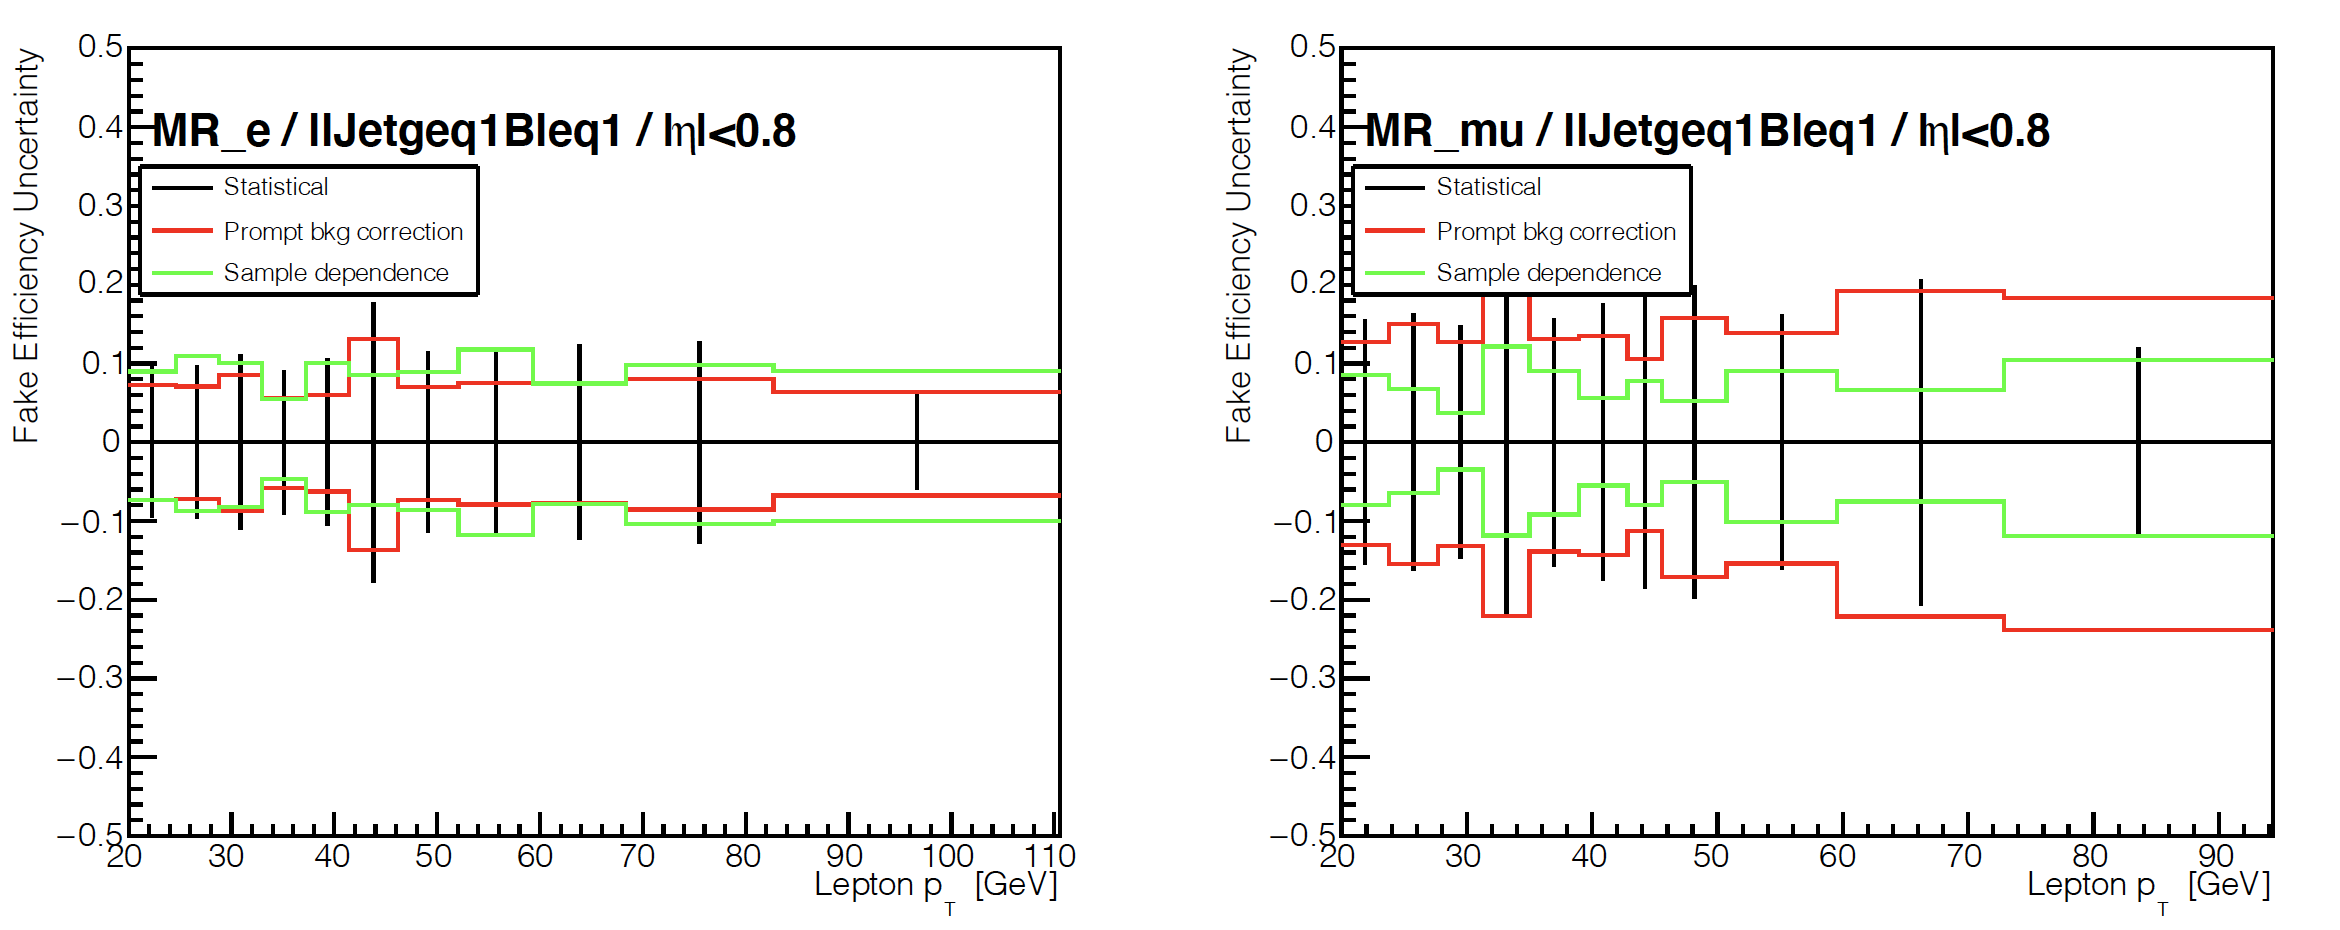
\includegraphics[width=0.99\textwidth]{figures/Part3/Systematics/MR2}
 \end{tabular}
 \caption{Comparison of different components of the uncertainties associated to the \emph{nonprompt} efficiency measured in 2017 dataset (njet$>$0 bin, $|\eta|<$0.8 bin). From left to right: electron $f$ uncertainty, muon $f$ uncertainty.}
 \label{fig:f_comp2}
 \end{center}
\end{figure}

Since the \emph{prompt} efficiency $r$ is measured in simulated $\ttbar$ events, \ac{MC} uncertainties described in \autoref{sec:OthUnc} are propagated to $r$ as the uncertainties. Additionally, statistical uncertainty is added in quadrature to the MC uncertainties to form the final uncertainty on $r$.

The uncertainties associated to the \emph{prompt} efficiency are relatively small when compared to the \emph{nonprompt} efficiency uncertainties. A comparison of different sources of \emph{prompt} efficiency uncertainties are shown in Figure \ref{fig:r_comp}.

\begin{figure}[tbh!]
 \begin{center}
 \begin{tabular}{c}
 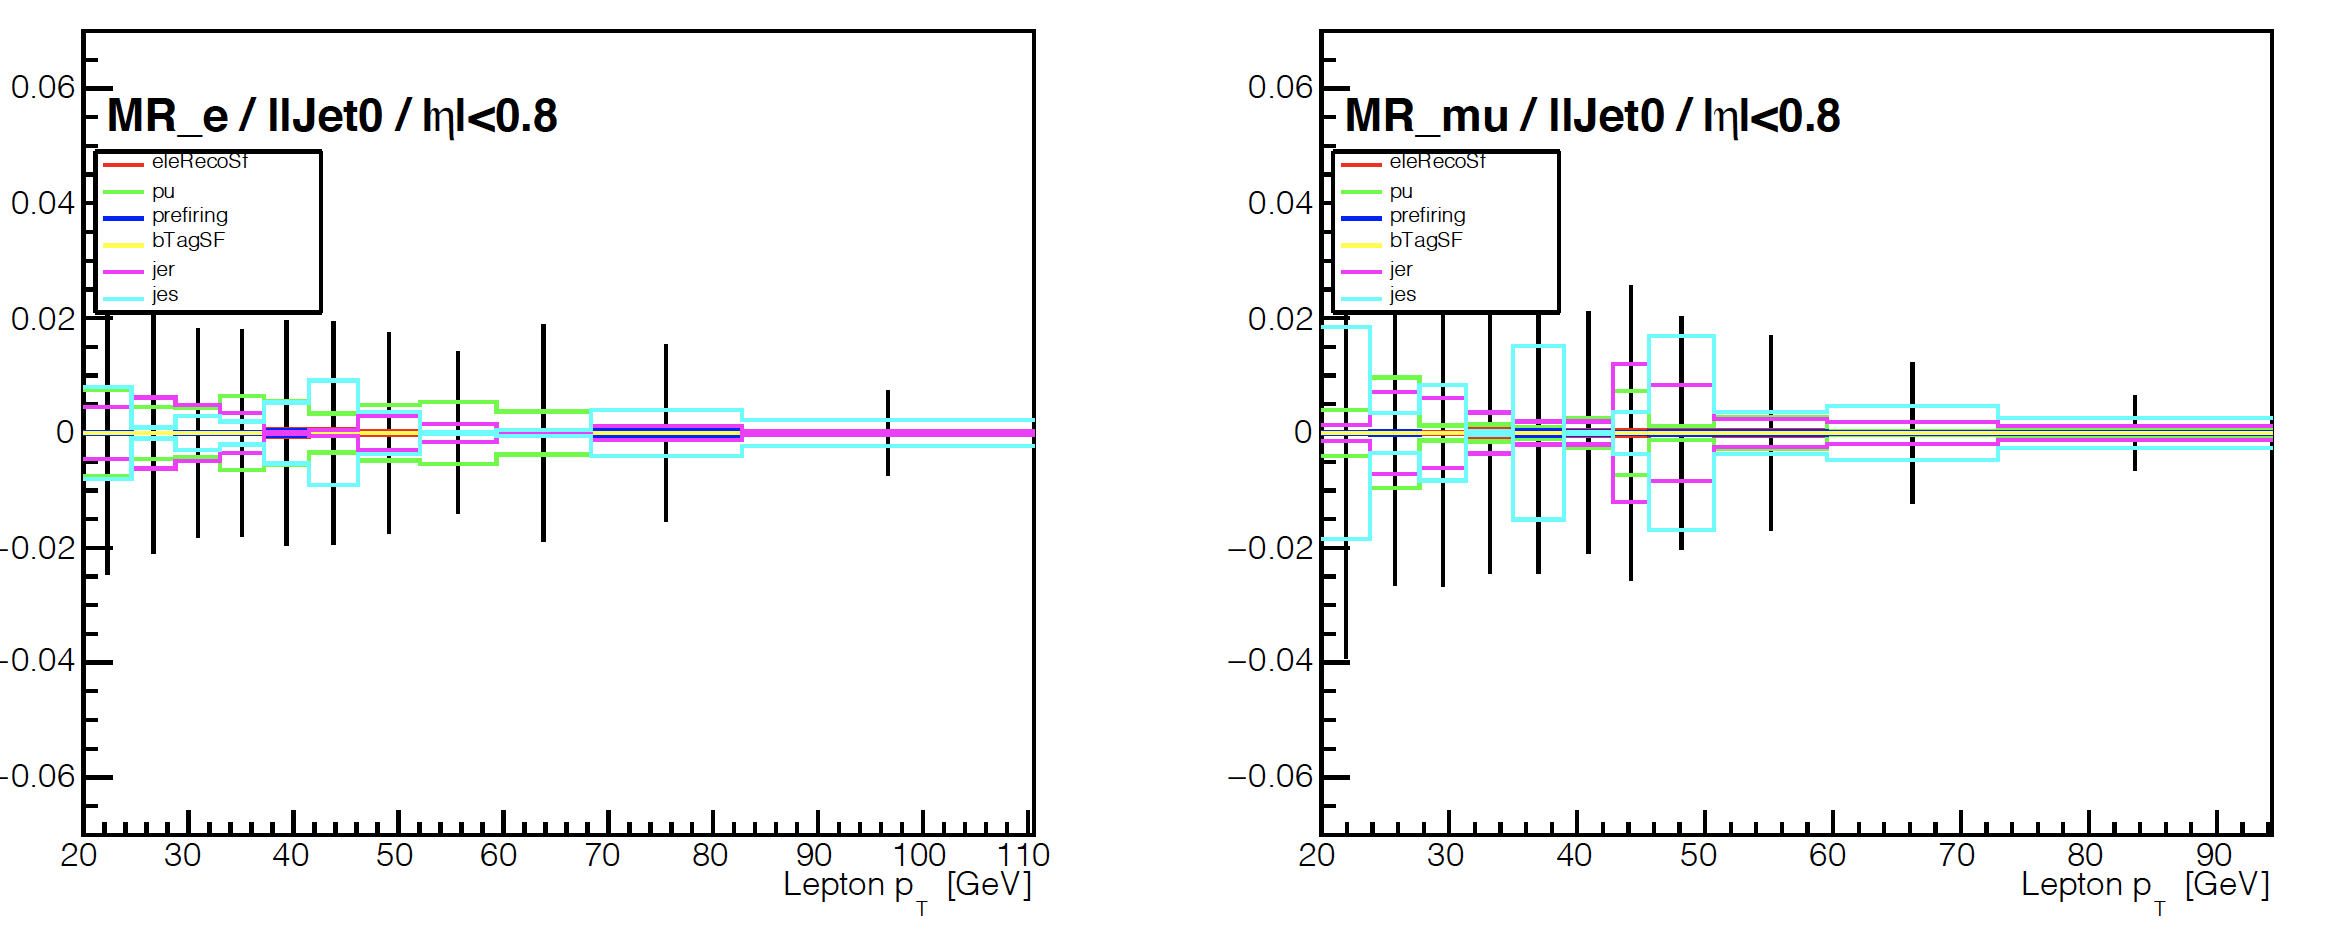
\includegraphics[width=0.99\textwidth]{figures/Part3/Systematics/MR}
 \end{tabular}
 \caption{Comparison of different components of the uncertainties associated to the \emph{prompt} efficiency measured in 2017 dataset (njet$=$0 bin, $|\eta|<$0.8 bin). From left to right: electron $r$ uncertainty, muon $r$ uncertainty.}
 \label{fig:r_comp}
 \end{center}
\end{figure}

Uncertainties associated to $r$ and $f$ are determined separately for electron and muon. Therefore, there are four independent uncertainties: $r_{\textsf{e}}$, $r_{\upmu}$, $f_{\textsf{e}}$ and $f_{\upmu}$. 

A fifth uncertainty is considered that accounts for the potential bias caused by the way the generalized matrix method is implemented. Four out of the eight \acp{AR} that appear on the lefthand side of the Equation \ref{eq:matrix_method3} (i.e. $N^{\overline{T}TT}$, $N^{\overline{T}T\overline{T}}$, $N^{\overline{T}\overline{T}T}$, $N^{\overline{T}\overline{T}\overline{T}}$) are selected by requiring the leading lepton in $\pt$ to fail the \emph{tight} criteria described in Table~\ref{tab:looseandtight}. Effectively this means that the isolation requirement is reversed for leading lepton that enter these four \acp{AR}. Selecting the leading lepton by a loose requirement is not ideal since the leading lepton is required to match with iso-triggers. To account for this bias, a 50 $\%$ uncertainty is assigned to the $f_1$ (\emph{nonprompt} efficiency associated to the leading lepton) for events that enter these four \acp{AR}. The variation of the \emph{nonprompt} estimate due to trigger matching is largely covered by this uncertainty, as is shown in Figure~\ref{fig:MM_trigger}.

\begin{figure}[tbh!]
 \begin{center}
 \begin{tabular}{cc}
 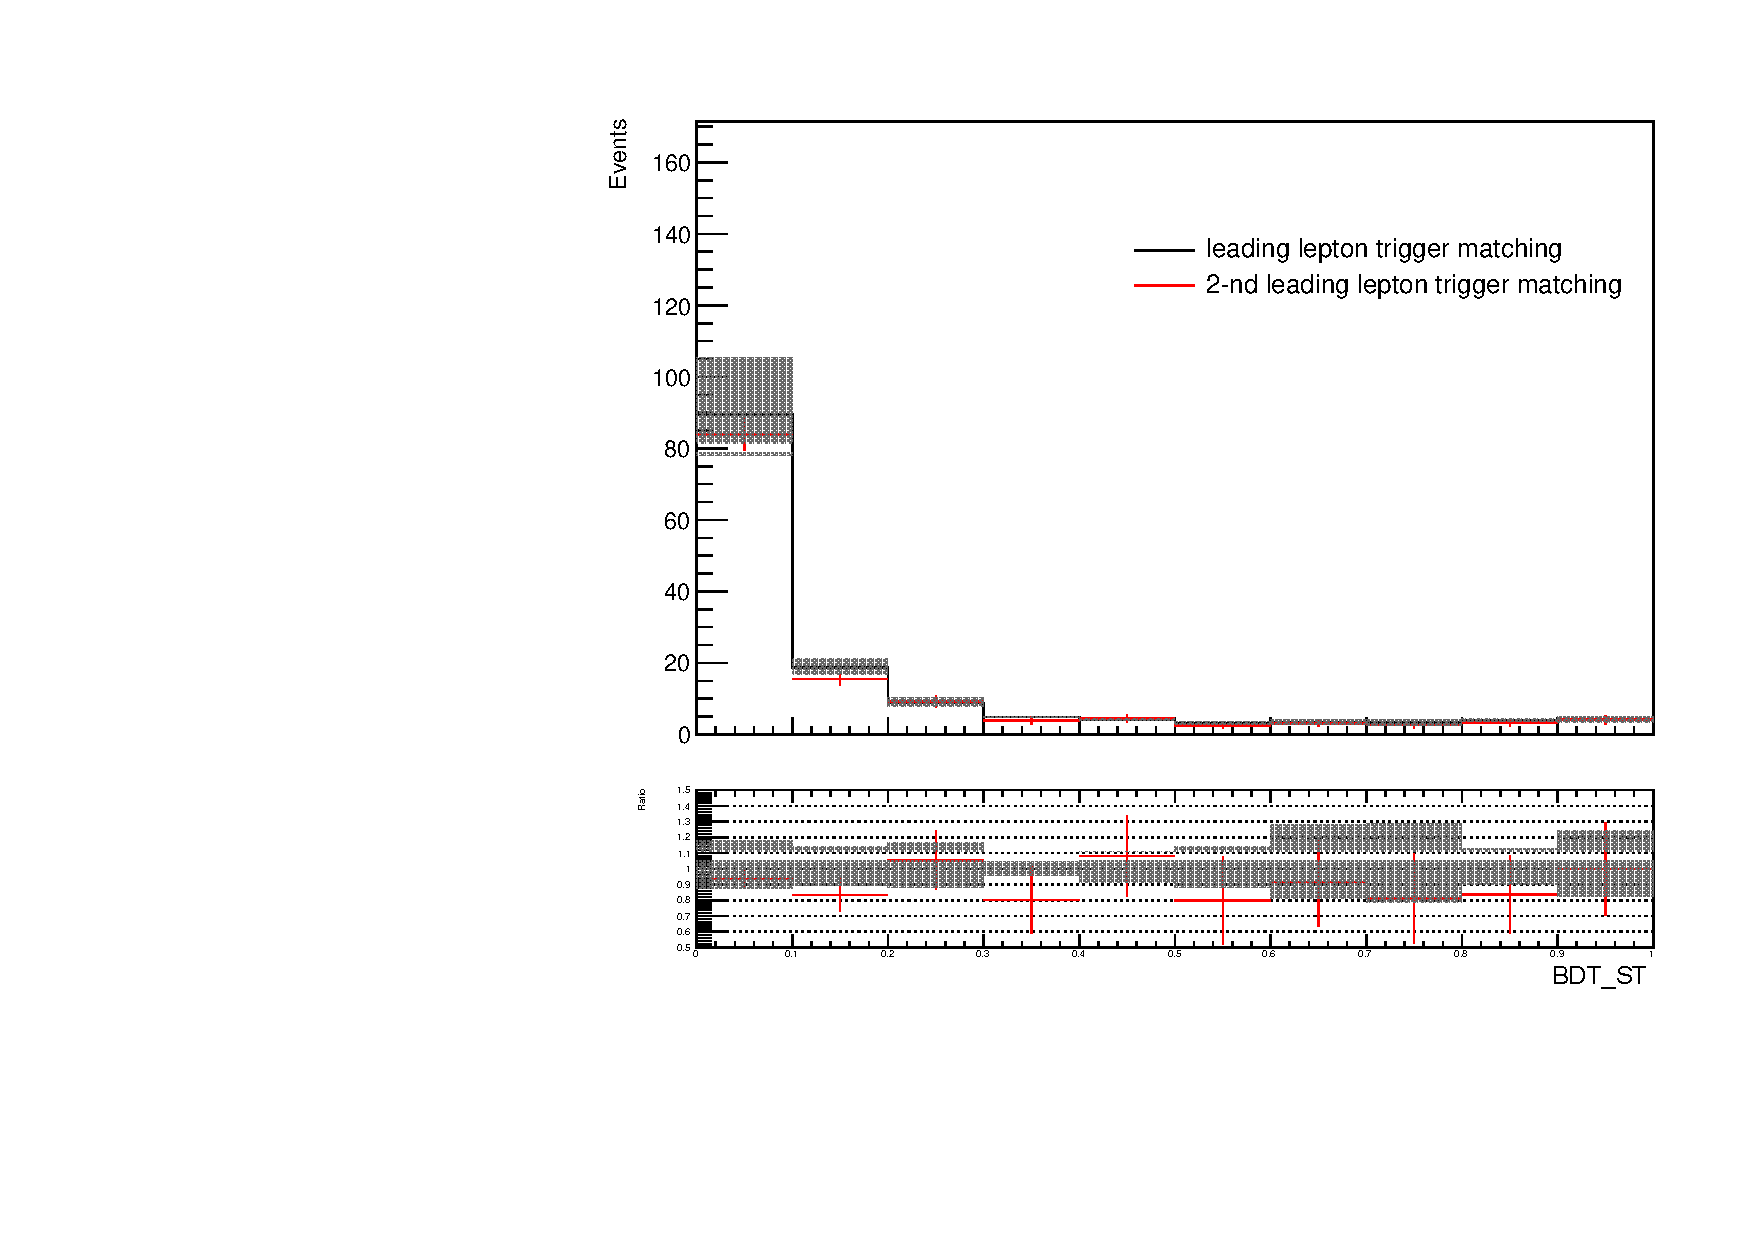
\includegraphics[width=0.47\textwidth]{figures/Part3/Systematics/BDT_ST_MM}&
 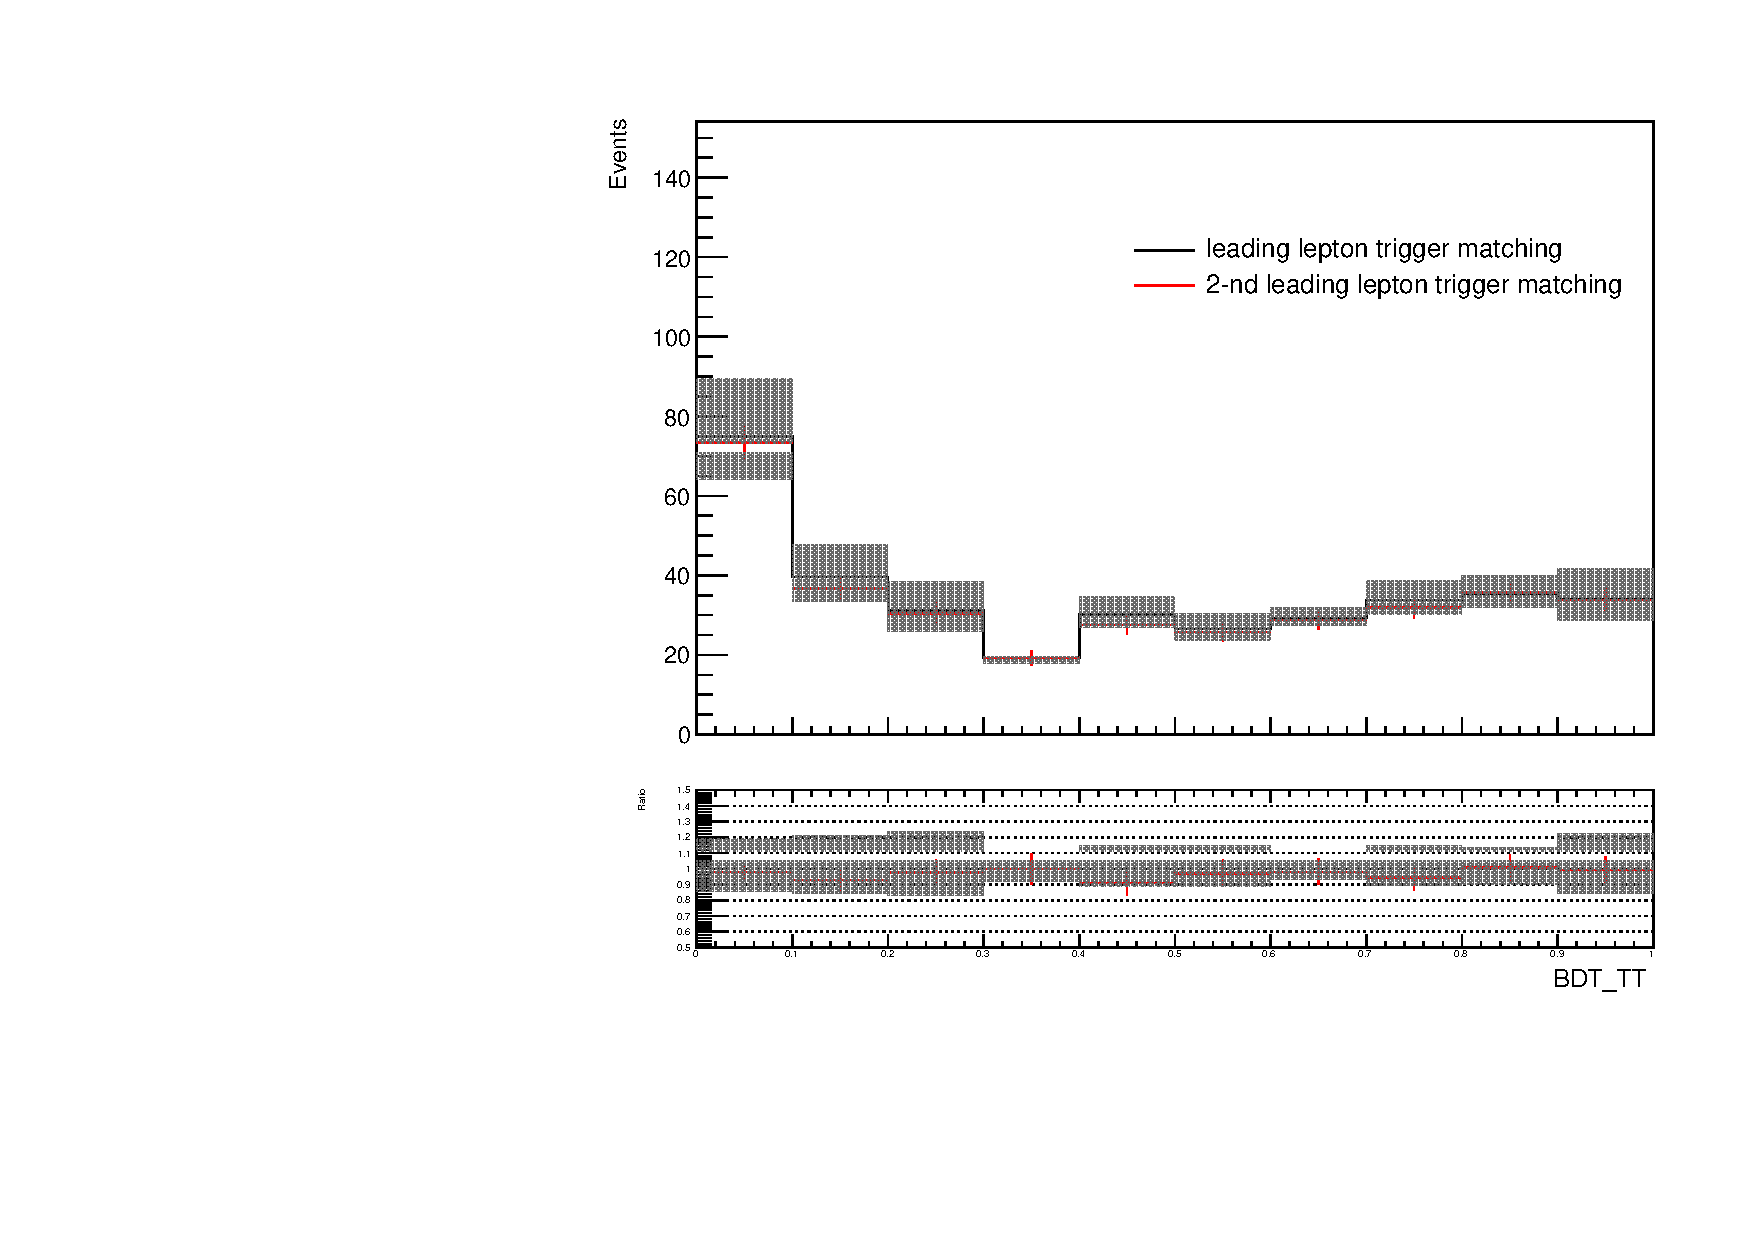
\includegraphics[width=0.47\textwidth]{figures/Part3/Systematics/BDT_TT_MM} \\
 \end{tabular}
 \caption{The impact of matching leptons to trigger objects on \emph{nonprompt} estimate. From left to right: \emph{nonprompt} estimate in top production enriched \ac{SR}, \emph{nonprompt} estimate in top decay enriched \ac{SR}. The nominal configuration of the matrix method is to match the leading lepton with trigger objects. Matching the sub-leading with the trigger objects is taken as an alternative to evaluate the robustness of the \emph{nonprompt} estimate. The uncertainty band only covers the variation of the \emph{nonprompt} estimate as a result of varying leading lepton $f$ by 50 $\%$. Uncertainty bars only include statistical uncertainties.}
 \label{fig:MM_trigger}
 \end{center}
\end{figure}

The five components of the uncertainties discussed in this section are propagated through the matrix inversion. The resulting variations of the \emph{nonprompt} estimates are taken as the uncertainties, which contain both normalization and differential effects to the BDT templates. These uncertainties are treated uncorrelated between different components but correlated between the years. In addition to these five uncertainties, an overall normalization uncertainty of 10$\%$ is assigned to cover any other potential variations of the \emph{nonprompt} backgrounds.
%%%%%%%%%%%%%%%%%%%%%%%%%%%%%%%%%%%%%%%%%%%%%%%%%%%%%%%%
%%%%%%%%%%%%%%%%%%%%%%%%%%%%%%%%%%%%%%%%%%%%%%%%%%%%%%%%

\section{Diboson Uncertainties}
\label{sec:DiUnc}

Mismodeling of the jet multiplicity is observed in WZ control region, as is shown in Figure~\ref{fig:WZ}. This is largely due to the fact WZ process is modeled at \ac{LO} with one extra parton in the \ac{ME}. Any other extra jets are modeled by the parton shower, which is suboptimal when compared to the modeling from \ac{ME}. To take this into account, a dedicated jet-dependent uncertainty is assigned to each event. This uncertainty is determined using diboson \ac{VR} that has the same OnZ requirement as the WZ \ac{VR}, no jet multiplicity requirement, a MET $>$ 85 GeV requirement, and a requirement of no b-tagged jets with $\pt$ $>$ 20 GeV. Unlike for the WZ \ac{VR}, events with different lepton flavor compositions are combined.

The jet multiplicity distributions in diboson \ac{VR} are shown in Figure~\ref{fig:VV_CR}. For each year, a scale factor parameterized as bins of jet multiplicity is derived,

\begin{equation}
\epsilon=\frac{N_{data}-N_{\textsf{VVV}}-N_{\textsf{t}\overline{\textsf{t}}+\textsf{X(X)}}-N_{\ttbar}-N_{others}}{N_{\textsf{VV}}}.
\end{equation}

\begin{figure}[tbh!]
 \begin{center}
 \begin{tabular}{ccc}
  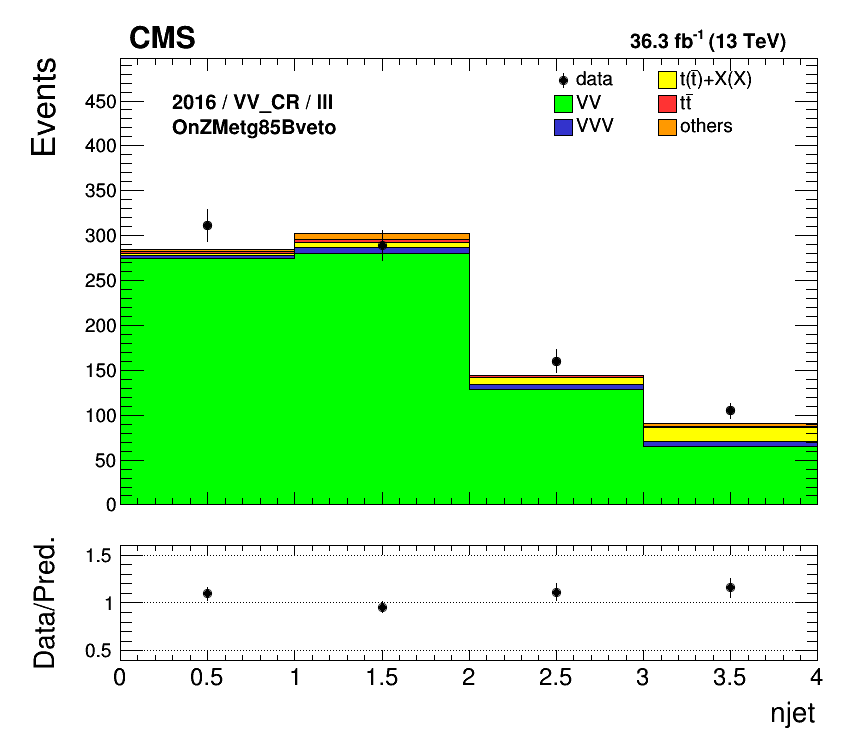
\includegraphics[width=0.325\textwidth]{figures/Part3/Systematics/njet_2016}&
    \includegraphics[width=0.325\textwidth]{figures/Part3/Systematics/njet_2017}&
  \includegraphics[width=0.325\textwidth]{figures/Part3/Systematics/njet_2018}\\
 \end{tabular}
 \caption{The diboson \acp{VR}, from left to right: 2016, 2017 and 2018 datasets.}
 \label{fig:VV_CR}
 \end{center}
\end{figure}

The scale factor $\epsilon$ is used to estimate the uncertainty, denoted by $\Delta$,

\begin{equation}
\Delta=|1-\epsilon|
\end{equation}

\begin{figure}[tbh!]
 \begin{center}
 \begin{tabular}{ccc}
  \includegraphics[width=0.325\textwidth]{figures/Part3/Systematics/2016_VV_Sys_1D}&
    \includegraphics[width=0.325\textwidth]{figures/Part3/Systematics/2017_VV_Sys_1D}&
  \includegraphics[width=0.325\textwidth]{figures/Part3/Systematics/2018_VV_Sys_1D}\\
 \end{tabular}
 \caption{Scale factors derived from the diboson \acp{VR}, from left to right: 2016, 2017 and 2018 datasets.}
 \label{fig:SF_VV}
 \end{center}
\end{figure}

This uncertainty shifts the predictions of WZ and ZZ processes by up to 20$\%$, as is shown in Figure \ref{fig:SF_VV}.
%%%%%%%%%%%%%%%%%%%%%%%%%%%%%%%%%%%%%%%%%%%%%%%%%%%%%%%%
%%%%%%%%%%%%%%%%%%%%%%%%%%%%%%%%%%%%%%%%%%%%%%%%%%%%%%%%

\section{Other Experimental Uncertainties}
\label{sec:OthUnc}

\begin{itemize}
\item Lepton reconstruction, identification, and isolation: electron/muon reconstruction uncertainties are provided by relevant POG. Uncertainties associated with lepton identification and isolation scale factors were evaluated by the authors of the mvaTOP ID cite{mvaTOP}. The statistical components of these uncertainties are treated as uncorrelated while the other components are treated as fully correlated. For high $p_{T}$ muons ($p_{T}>$200GeV), an additional uncertainty (denoted ``muIDHighPt") is assigned and it increases linearly from 0 to 10$\%$ (200GeV-1000GeV) and is caped at $10\%$ after 1000GeV.
\item Muon scale uncertainties: uncertainties on muon momentum (denoted ``MuonScale") are assigned using different method according to the muon $p_{T}$: Rochester algorithm is used for low $p_{T}$ muons ($p_{T}<$200Gev), while GEcite{GEmethod} method is used for high $p_T$ muons ($p_{T}>$200Gev).
\item b-tagging: b-tagging efficiency and uncertainty is provided by the BTV group. 
\item trigger scale factor: trigger scale factors are set to 1 and a flat 2$\%$ uncertainty is assigned. This uncertainty is treated as uncorrelated.
\item Luminosity: The uncertainties of 1.0$\%$, 2.0$\%$ and 1.5$\%$  are assigned to the integrated luminosity for 2016, 2017, 2018, respectively. When processing the run 2 data the individual year uncertainties are treated as uncorrelated while there are two additional correlated luminosity uncertainties; firstly, 0.6$\%$, 0.9$\%$ and 2.0$\%$ for each year respectively to account for the correlation between 2016, 2017 and 2018 data and secondly, 0.6$\%$,0.2$\%$ for 2017 and 2018 respectively to account for the correlation between 2017 and 2018 data. 
\item jet energy scale and resolution: The jet energy scale, JES, and jet energy resolution, JER, are centrally provided by the JET/MET POG cite{JEC}. Variations of jet energy scale and resolution are propagated to the MET and b-tagging SF.
\item pile-up reweighting: The measured minimum bias cross-section is varied up and down by 4.6$\%$. This uncertainty is treated as correlated. 
\item MET unclustered missing energy is considered and treated as uncorrelated across the years.
\item L1 ECAL prefiring: In the 2016 and 2017 datasets, L1 EGamma triggers fired early causing many uninteresting events to be recorded while the later interesting events were rejected. Since this effect is not present in the MC simulation, a tool cite{ECALPre} provided by the L1 DPG is used to reweight MC events. This uncertainty is treated as correlated. 
\item HEM15/16 Issue: The HEM15/16 issue refers to two HCAL modules whose power supply died in 
the middle of the data taking (runs$>=$319077, i.e. last certified run of 
2018B, and all of 2018C+D). The HEM issue is likely a very small effect but we still have to check it following the procedure in cite{HEM}
\end{itemize}

Uncertainties related to B-tagging scale factors are split into different sources. For b and udsg jets, we applied lf, hf, hfstats1/2, and lfstats1/2 uncertainties. For c jets, we applied cferr1/2 uncertainties. Correlations between different sources are specified in the Table~\ref{tab:btagsys}.

\begin{table}[!hbtp]
\sffamily
\centering
\caption{
A hyphen ($-$) denotes that a source is not correlated between the different years.
}
\begin{tabular}{lcl}
\toprule
Source & Correlated & Description\\
\midrule
lf			& \checkmark & udsg+c jets in heavy flavor region\\ %HF$^1$
hf			& \checkmark & b+c jets in light flavor region \\ %LF$^2$
hfstats1	& - 		 & Linear fluctuations of c jets\\
hfstats2	& -			 & Quadratic fluctuations of c jets \\
lfstats1	& -			 & Linear fluctuations of udsg jets \\
lfstats2	& -			 & Quadratic fluctuations of udsg jets \\
cferr1		& \checkmark & Linear fluctuations of c jets \\
cferr2		& \checkmark & Quadratic fluctuations of c jets \\
\bottomrule
\end{tabular}
\label{tab:btagsys}
\end{table}

\subsection{Jet energy scale uncertainties}

Uncertainties associated with JES are split into their 27 components and properly treated the correlations of the split uncertainties by year as recommended by the JETMET POG and described in the Table \ref{tab:jec}.

\begin{table}[!hbtp]
\sffamily
\centering
\caption{
Summary of the sources of uncertainty related to the JECs.
A hyphen ($-$) denotes that a source is not correlated between the different years.
}
\label{tab:jec}
\begin{tabular}{lc|lc}
\toprule
Source & Correlated & Source & Correlated \\
\midrule
AbsoluteStat			& -		&	 RelativePtHF			& \checkmark			 \\
AbsoluteScale			& \checkmark		&	 RelativeBal				& \checkmark			 \\
AbsoluteMPFBias			& \checkmark 	&	 RelativeSample			& -			 \\	 
Fragmentation			& \checkmark		&	 RelativeFSR				& -			 \\
SinglePionECAL			& \checkmark	&	 RelativeStatFSR			& \checkmark			 \\	 
SinglePionHCAL			& \checkmark	&	 RelativeStatEC			& -			 \\	 
FlavorQCD				& \checkmark	&	 RelativeStatHF			& -			 \\	 
TimePtEta				& -			 &          PileUpDataMC			& \checkmark			 \\
RelativeJEREC1			& -		&	    PileUpPtRef				& \checkmark			 \\
RelativeJEREC2			& -		&	    PileUpPtBB				& \checkmark			 \\
RelativeJERHF			& \checkmark		&	 PileUpPtEC1				& \checkmark			 \\
RelativePtBB			& \checkmark		&	 PileUpPtEC2				& \checkmark			 \\
RelativePtEC1			& -			&     PileUpPtHF				& \checkmark			 \\
RelativePtEC2			& -			&     & \\
\bottomrule
\end{tabular}
\end{table}

B-tagging scale factors and MET vector are computed for each of the JES templates and treated as uncertainties that are fully correlated to the respective JES sources. 

The overall systematic uncertainty on background is estimated to be about 15 $\%$ in SR.

 A comparison of different sources of systematic uncertainties of the background estimates in SR is shown in Figure \ref{fig:Comp_sys_background}.

\begin{figure}[tbh!]
 \begin{center}
 \begin{tabular}{cc}
    \includegraphics[width=0.45\textwidth]{figures/Part3/Systematics/sysBDT_ST_bkg_2017}&
  \includegraphics[width=0.45\textwidth]{figures/Part3/Systematics/sysBDT_TT_bkg_2017} \\
 \end{tabular}
 \caption{Distributions of relative uncertainties on total expected backgrounds as a function of BDT output in ST enriched SR (left), TT enriched SR (right). Luminosity and normalization uncertainties are not included in these plots. JES, JER and HEM are combined into "JEC". Sources of b-tagging uncertainties listed in Table~\ref{tab:btagsys} are combined into "BtagSF".}
 \label{fig:Comp_sys_background}
 \end{center}
\end{figure}

 A comparison of different sources of systematic uncertainties of the signal estimates in SR is shown in Figure \ref{fig:Comp_sys_signal}.

\begin{figure}[tbh!]
 \begin{center}
 \begin{tabular}{cc}
    \includegraphics[width=0.45\textwidth]{figures/Part3/Systematics/sysBDT_ST_sig_2017}&
  \includegraphics[width=0.45\textwidth]{figures/Part3/Systematics/sysBDT_TT_sig_2017} \\
 \end{tabular}
 \caption{Distributions of relative uncertainties on signal ($C_{e\mu tu}^{vector}$ is used as an example) as a function of BDT output in ST enriched SR (left), TT enriched SR (right). Luminosity and normalization uncertainties are not included in these plots. JES, JER and HEM are combined into "JEC". Sources of b-tagging uncertainties listed in Table~\ref{tab:btagsys} are combined into "BtagSF".}
 \label{fig:Comp_sys_signal}
 \end{center}
\end{figure}

Representative range of systematic uncertainties on background and signal MC samples are summarized in cite{SysError}. These uncertainties are extracted from the last bins of the BDT distribution.
\chapter{Statistical Analysis}
\label{chap:Results}

In the absence of significant excess over the \ac{SM} prediction, the observed distributions of the \ac{BDT} discriminator are used to test various hypophyses, where the coexistence of the \ac{CLFV} signals and backgrounds are assumed. A statistical method called ``profile likelihood'' is used to move the focus on the cross sections of the \ac{CLFV} signals while also keeping track of the systematic uncertainties. The profile likelihood fit performed on the distributions of the \ac{BDT} discriminator is discussed in \autoref{sec:PLF}. Upper limits on various \acp{WC} and branching fractions established by this analysis are presented in \autoref{sec:Limits}. 
%%%%%%%%%%%%%%%%%%%%%%%%%%%%%%%%%%%%%%%%%%%%%%%%%%%%%%%%%%%
%%%%%%%%%%%%%%%%%%%%%%%%%%%%%%%%%%%%%%%%%%%%%%%%%%%%%%%%%%%

\section{Profile Likelihood Fit}
\label{sec:PLF}

A binned likelihood function $\mathcal{L}(\mu, \theta)$ is constructed to perform the statistical analysis using the \ac{BDT} discriminator distributions. The top quark production and decay signal modes are combined. The signal strength $\mu$, defined previously in Equation~\ref{eq:signal_strength}, governs the cross-section of the two signal modes simultaneously. 

All systematic uncertainties are incorporated into the likelihood function as nuisance parameters, denoted by $\theta$. The uncertainties that affect the shape of the \ac{BDT} discriminator distributions utilize Gaussian distributions while other uncertainties that only affect the normalizations utilize log-normal distributions. The ``Barlow-Beeston lite'' method \cite{Barlow:1993dm} is used to incorporate the statistical uncertainties in the signal and background predictions. 

A profile likelihood fit is performed simultaneously in six regions (three data-taking years and two \acp{SR}) by maximizing the likelihood function $\mathcal{L}(\mu, \hat{\theta}_{\mu})$, where $\hat{\theta}_{\mu}$ are the values of the nuisance parameters that maximize the likelihood for a specific signal strength. The post-fit distributions of the \ac{BDT} discriminators are shown in Figure~\ref{fig:bdt_postfit_VecU}. The largest post-fit uncertainties are the statistical uncertainties from the limited number of simulated events.

\begin{figure}[tbh!]
 \begin{center}
 \begin{tabular}{cc}
 \includegraphics[width=0.48\textwidth]{figures/Part3/Results/BDT_TT_VecU}&
 \includegraphics[width=0.48\textwidth]{figures/Part3/Results/BDT_ST_VecU}\\
 \end{tabular}
 \caption{Distributions of the post-fit \ac{BDT} discriminator targeting the \ac{CLFV} top quark decay (left) and production (right) signal. Contributions from the two signal modes (production and decay) are combined within each \ac{SR} and are shown as the solid red line. The post-fit signal strength ($\mu_{\emut{u}}^{\textsf{vector}}=\hat{\mu}_{\emut{u}}^{\textsf{vector}}$) is used to normalise the signal cross sections. The hatched bands indicate post-fit uncertainties (statistical and systematic) for the SM background predictions.}
 \label{fig:bdt_postfit_VecU}
 \end{center}
\end{figure} 

The impacts of the nuisance parameters on the profile likelihood fit are quantified and a representative ranking of the impacts is shown in Figure~\ref{fig:Impact}. In general, the most prominent uncertainties affecting the likelihood fit are the statistical uncertainties that arise from limited sample size. A full collection of nuisance parameter impacts can be found in \autoref{chap:Impact}.

\begin{figure}[tbh!] 
\begin{center}
\includegraphics[width=0.9\textwidth]{figures/Part3/Results/Impact_VecU}
 \caption{The nominal value of the observed signal strength $\hat{\mu}$ and its uncertainty is shown in the top right corner. Ranking of the nuisance parameters according to their observed impacts on $\hat{\mu}$ (represented with error bars) is shown in the right panel. Only the 10 nuisance parameters with the largest observed impacts are shown. The expected impacts (represented with red and blue rectangles) are derived using Asimov fits, where data is replaced by a background-only template (i.e. the nominal value of the expected $\hat{\mu}$ is 0). The impact of each nuisance parameter, $\mathrm{\Delta}\hat{\mu}$, is calculated as the difference between the nominal $\hat{\mu}$ and the value of $\hat{\mu}$ when the corresponding nuisance parameter is fixed to $\hat{\theta}\pm\sigma$, where $\hat{\theta}$ ($\sigma$) is its post-fit value (uncertainty). The left panel shows the pulls (represented with black dots) and uncertainties (represented with error bars and grey rectangles) of the nuisance parameters in units of the pre-fit uncertainties. The pulls are calculated as the difference between the nominal and the post-fit values of the nuisance parameters. The ``\ac{SR}2'' quoted in the label corresponds to the top quark production enriched signal region.}
 \label{fig:Impact}
 \end{center}
\end{figure}
%%%%%%%%%%%%%%%%%%%%%%%%%%%%%%%%%%%%%%%%%%%%%%%%%%%%%%%%%%%
%%%%%%%%%%%%%%%%%%%%%%%%%%%%%%%%%%%%%%%%%%%%%%%%%%%%%%%%%%%

\section{Upper Limits}
\label{sec:Limits}

The compatibility between the data and the combined signal plus background expectation under the hypothesized value of the signal strength $\mu$ is quantified by a test statistic that considers the profile likelihood ratio:

\begin{equation}
q(\mu)=-2\ln\frac{\mathcal{L}(\mu,\hat{\theta}_{\mu})}{\mathcal{L}(\hat{\mu},\hat{\theta})}.
\end{equation}

Using the asymptotic modified frequentist CL$_{s}$ method~\cite{Junk:1999kv,Read2002,Cowan:2010js} with the profile likelihood ratio as the test statistic, upper limits are placed on $\mu$ at 95\% \ac{CL}. The one-dimensional upper limits on a given \ac{WC}, $\WC{}{a}/\Lam^2$, are obtained by taking the square root of the corresponding signal strength $\mu_a$ while setting other \acp{WC} to zero. The branching fractions, $\mathcal{B} (\tto{q})$ with q=u or c, are obtained assuming a top quark mass (width) of 172.5 (1.33) GeV in Equation~\ref{eq:4} taken from~\cite{Kile:2008rp}.

The resulting one-dimensional limits are summarized in Table~\ref{tab:limit}. Assuming a linear relationship between $\mathcal{B}(\tto{u})$ and $\mathcal{B}(\tto{c})$ in the case of nonvanishing signals, the two-dimensional limits can be obtained through interpolation and are shown in Figure~\ref{fig:2dlimit}. 

\begin{table}[th]
\sffamily
\centering
\caption{Upper limits at 95\% \ac{CL} on \acp{WC} and the branching fractions. The expected and observed upper limits are shown in regular and bold fonts, respectively. The intervals that contain 68\% of the distribution of the expected upper limits are shown in parentheses.}
\resizebox{0.95\linewidth}{!}{%
\begin{tabular}{cccccc}
\toprule
CLFV & Lorentz & \multicolumn{2}{c}{$\WC{}{\emut{q}}/\mathrm{\Lam}^2~(\TeV^{-2})$} & \multicolumn{2}{c}{$\mathcal{B} (\tto{q}) \times 10^{-6}$} \\
coupling & structure & Exp. (68\% range) & Obs. & Exp. (68\% range) & Obs. \\
\midrule
\multirow{3}{*}{$\emut{u}$}& Tensor & 0.022 (0.018--0.026) & \textbf{0.024} & 0.027 (0.018--0.040) & \textbf{0.032}\\
& Vector & 0.044 (0.036--0.054) & \textbf{0.048} & 0.019 (0.013--0.028) & \textbf{0.022}\\
& Scalar & 0.093 (0.077--0.114) & \textbf{0.101} & 0.010 (0.007--0.016) & \textbf{0.012}\\
\midrule
\multirow{3}{*}{$\emut{c}$} & Tensor & 0.084 (0.069--0.102) & \textbf{0.094} & 0.396 (0.272--0.585) & \textbf{0.498}\\
 & Vector & 0.175 (0.145--0.214) & \textbf{0.196} & 0.296 (0.203--0.440) & \textbf{0.369}\\
 & Scalar & 0.385 (0.318--0.471) & \textbf{0.424} & 0.178 (0.122--0.266) & \textbf{0.216}\\
 \bottomrule
\end{tabular}
}
\label{tab:limit}
\end{table}

\begin{figure}[tbh!]
 \begin{center}
 \begin{tabular}{cc}
 \includegraphics[width=0.48\textwidth]{figures/Part3/Results/Hist2D_WC}&
 \includegraphics[width=0.48\textwidth]{figures/Part3/Results/Hist2D_BR}\\
 \end{tabular}
 \caption{Two-dimensional 95$\%$ \ac{CL} upper limits on the \acp{WC} (left) and the branching fractions (right). The observed (expected) upper limits for tensor-, vector-, and scalar-like \ac{CLFV} interactions are shown in red, blue, and black solid (dotted) lines, respectively. The shaded bands contain $68\%$ of the distribution of the expected upper limits.}
 \label{fig:2dlimit}
 \end{center}
\end{figure}